\documentclass[12pt]{report}
\usepackage[top=2.5cm, bottom=2.5cm, left=3cm, right=2.5cm, centering]{geometry}
% \setcounter{secnumdepth}{2} % livello massimo di sezionamento numerato
% Interlinea
\linespread{1.2}
\usepackage[italian]{babel} % applicazione regole di scrittura
\usepackage{float} % per il posizionamento delle immagini
\usepackage{listings} % per il codice di programmazione
% \usepackage[utf]{inputenc}
\usepackage{fontspec}
\usepackage{graphicx}
\usepackage{subfig}
\usepackage{float}
\usepackage[font={footnotesize,it}]{caption}
\usepackage[colorlinks=true,linkcolor=black,anchorcolor=black,citecolor=blue,filecolor=black,menucolor=black,runcolor=black,urlcolor=black]{hyperref}
\usepackage{enumitem}
% \setlist{nosep} % or \setlist{noitemsep} to leave space around whole list
\setlist{noitemsep}

\usepackage[squaren]{SIunits} %per angstrom
\usepackage{amssymb} %simboli
 
\usepackage[
left = \flqq{},% 
right = \frqq{},% 
leftsub = \flq{},% 
rightsub = \frq{} %
]{dirtytalk} % quotes

\usepackage[backend=biber,style=ieee,sorting=none]{biblatex}
\addbibresource{bibliografia.bib}

\begin{document}
	
\author{Ludovico Venturi}
\title{Tesi Triennale in Informatica}
	
% Frontespizio
\begin{titlepage}
	\begin{figure}
		\centering
\includegraphics[scale=0.2] {images/UNIPI_Logo.png}
	\end{figure}
	
	\begin{center}
		{\LARGE{ Corso di Laurea Triennale in Informatica (L-31) \\}}
		\vspace{2cm}
		{\Large { TESI DI LAUREA }}\\
		\vspace{2cm}
		{\LARGE { \textbf{Protein Folding: dai metodi classici per la predizione della struttura di proteine alla rivoluzione di AlphaFold} }}
	\end{center}
	
	\vspace{2cm}
	
	\begin{minipage}[t]{0.6\textwidth}
		{\large{\textbf{Relatore}\\ Prof. Paolo\textbf{ Milazzo}}}\\ \\
		{\large{\textbf{Correlatore}\\ Prof. Mario\textbf{ Pirchio}}}
		\vspace{0.5cm}
	\end{minipage}\hfill
	\begin{minipage}[t]{0.3\textwidth}\raggedleft
		\vspace{1.33cm}
		{\large{\textbf{Candidato} \\ Ludovico \textbf{Venturi}\\ }}
	\end{minipage}
	
	\vspace{25mm}
	
	\centering{\large{\bf ANNO ACCADEMICO 2020/2021 }}
\end{titlepage}
% Fine frontespizio

\tableofcontents
\clearpage

% Trasformare l’esperienza dell’università in qualcosa di positivo, di progressivo, che può alimentare il fuoco delle mie passioni
Fai qualcosa di specifico, renditi esperto.\newline

Guida il lettore da 0 ad Alphafold facendolo meravigliare davanti alla bellezza della bioinformatica, e della vita.\newline

Medita e poi scrivi qui: non passare da fonti terze. Non perdere il flusso.\\
Tu stai scrivendo qualcosa per te, non per il mondo. Scrivi, poi confrontati. Se ti confronti è normale che ti vedi inferiore. Come puoi invece essere inferiore a te stesso? \newline

Ciò che conta è fare, fare, fare, mettere in pratica.\newline

Hai scelto tu di uscire dall’informatica. Hai paura di risultare ignorante in biologia? Hai paura di esserti immischiato in un campo a te esterno e di sembrare “capiscione”? \\
1. Non ne sa quasi nulla nessuno dei prof 2.Non interessa loro 3. ho Mario Pirchio a cui chiedere aiuto 4. voglio uscire dall’informatica pura. Non mi fido. Non mi interessa. Qui mi interesso 5.affronta la responsabilità. Ho la responsabilità di creare la mia strada e crederci, di laurearmi per mio padre e la mia famiglia.\newline

Mentre disegnavo ho notato che ciò che mi spingeva a a migliorare il disegno era riuscire a intravedere il risultato finale in quello che stavo facendo. Non stavo tracciando una linea su un foglio. Stavo facendo piccoli passi per mettere su carta ciò che vedevo dentro di me (non nella mente, ma nel cuore).\\ Realizzavo una piccola parte di me al di fuori di me. E vedere che ciò che stavo creando si stava avvicinando a ciò che avevo in mente mi dava una soddisfazione immensa. E questa felicità mi spingeva tantissimo a continuare e a migliorarmi.\\
Voglio scrivere questo documento per realizzare una piccola parte di me all’esterno di me.\\
L’obiettivo del disegno era realizzare un ritratto di Thich Nhat Hanh, per esprimere la mia gratitudine nei suoi confronti.\newline

Obiettivo finale: realizzare un documento riguardante il background della bioinformatica e lo studio di AlphaFold per esprimere la mia speranza che l’informatica possa essere usata per il bene della Vita, che ci possa avvicinare ad una comprensione maggiore di essa e di quanto ogni fenomeno sia interrelato.\newline

La tesi serve a dimostrare una ipotesi che avete elaborato dall’inizio, non a mostrare che voi sapete tutto

Ludo non dimenticarti quanta luce hai, sei ricco di una bellezza tanto speciale, non lasciare che altri te la nascondano\\
... \textit{ti ringrazio per ciò che sei}...\\
Tutto ciò che sei, che dici, che fai è meraviglioso\\
Dovresti sentirti in colpa con te stesso se invece abbandonassi tutto e tornassi a casa per paura di sbagliare\\
Ludo non hai bisogno di me, nè di tua madre nè di nessun altro. Tu sei una persona davvero meravigliosa, sei forte, hai tanta luce in te. Una cosa che penso di sapere è che potresti fare qualsiasi cosa, andare da qualsiasi parte. E se lo vorrai io ci sarò in ogni caso, non hai bisogno del mio appoggio per raggiungere quello che vuoi, ma io sono qui, e ci resto per tutto il tempo che vorrai.\\
E potessi starti vicina ogni notte e risvegliarmi accanto a te la mattina farei il tifo per te direttamente dalla prima fila ;")\\
ci credo davvero nel risultato positivo che potrai scoprire tra un po', non demordere prima o poi arriverà esattamente quella cosa che stavi aspettando e tutto andrà a posto da sè [..Sophie..]\\ \\

Una cosa per volta. Svuota il cervello. Adesso il mondo ti sembra pieno di problemi. Ne esiste solo uno per te: il tuo obiettivo. Se pensi a tutte le possibilità rimani fermo. Va solo in direzione dell'obiettivo. Poi al prossimo ci si penserà una volta raggiunto. Nessuno ti mette i bastoni fra le ruote, siamo con te. [papà] \\ \\


Non solo hai dato voce alla tua vita, ma sei stato in grado di renderla poesia, sono veramente orgoglioso di te e di come ti ho rivisto dopo tanto tempo perché, te lo dico con tutto il cuore, hai fatto dei passi da gigante, dei passi enormi e veramente complimenti. [..diego] \\ \\
Quando l'ansia bussa alla porta ringhio contro di lei: "ti affronto". Sono qui, avanti. Mi fermo e la guardo negli occhi. Affronto la vita, senza scappatoie. \\

Non abbiate paura di rischiare per non sbagliare. Mordete la vita. Sporcatevi le mani [Mattarella] \\
\clearpage
% % \addcontentsline{toc}{chapter}{Riassunto} % Capitolo non numerato
	
	\vspace*{\fill}
	\begin{center}
		\textbf{\LARGE Riassunto}\newline\newline
	\end{center}
	\begin{list}{}{
			\leftmargin=.2\textwidth
			\rightmargin=.2\textwidth
			\listparindent=\parindent
			%\itemindent=\parindent
			\itemsep=0pt
			\parsep=0pt}
		\item\relax
			Va posto al centro della seconda pagina e non dovrebbe superare le 20 righe.\\
			Va posto al centro della seconda pagina e non dovrebbe superare le 20 righe.
			Va posto al centro della seconda pagina e non dovrebbe superare le 20 righe.\\
			\par Va posto al centro della seconda pagina e non dovrebbe superare le 20 righe.
			Va posto al centro della seconda pagina e non dovrebbe superare le 20 righe.\\
			Va posto al centro della seconda pagina e non dovrebbe superare le 20 righe.\\
			Va posto al centro della seconda pagina e non dovrebbe superare le 20 righe.
		
	\end{list}
	\vfill % equivalent to \vspace{\fill}
	\clearpage



\clearpage % Riassunto

% \chapter{Acapitolo - riposiziona il mio contenuto}

\addcontentsline{toc}{chapter}{Introduzione}

\textbf{{\LARGE Introduzione\newline\newline L'informatica: un potente strumento}}
\vspace{1cm}

Illustrare il mio obiettivo e la suddivisione del lavoro, dopo aver esposto la mia posizione sui rischi e le prospettive positive aperte dall'informatica.\\\\


-- continua l;'introduzione dall'aritcolo: Soft computing methods for the prediction of protein tertiary
structures: A survey --


- Soft computing
I paradigmi del soft computing per la predizione della struttura delle proteine sono:
\begin{itemize}
\item ANNs: artificial neural networks
\item EC: evolutionary computation
\item SVMs: support vector machines
\end{itemize}
Inoltre i metodi per la predizione della struttura delle proteine possono essere ulteriormente classificati in base ad un'approssimazione biologica \cite{marquez2015soft}:
\begin{itemize}
	\item homology-based methods
	\item threading methods
	\item \textit{ab initio } methods
\end{itemize}


\section{Background filosofico}
Buttaci un po' di filosofia della scienza e di quali cambiamenti potrebbe apportare alla struttura delle rivoluzioni scientifiche. Cita Fleck in qualche modo!
Trova casi di cambi di paradigma e a "riscoperte" tornate alla ribalta grazie all'informatica. Magari l'informatica è un modo, analizzando tanti dati, di contrastare i bias nella scienza?



\section{Determinazione sperimentale della struttura delle proteine}

Ci sono 3 tecniche sperimentali che possono essere usate per generare informazioni a risoluzione atomica sulla struttura delle proteine.

\subsection{Valutazione dell'accuratezza delle predizioni}

Le tecniche di valutazione della predizione della struttura delle proteine richiede criteri ogettivi sulla similarità tra un modello computazionale e la struttura di riferimento determinata sperimentalmente.\\

La misura di valutazione dell'accuratezza oggi è utilizzata è il lDDT (\textit{local Distance
	Difference Test}) \cite{mariani2013lddt}. \\

Le misure precedenti si basavano su una superposizione globale di atomi di carbonio ed erano fortemente influenzate dai movimenti di dominio e non assicurano l'accuratezza di detagli atomici locali nel modello.



\chapter{AlphaFold}
AlphaFold è un sistema di \textit{Artificial Intelligence }(AI) sviluppato da DeepMind che realizza predizioni allo stato dell'arte sulla struttura delle proteine basandosi sulle loro sequenze amminoacidiche.

\section{DeepMind}

DeepMind è un'azienda inglese di Intelligenza Artificiale sussidiaria di Alphabet Inc.; in altre parole DeepMind è una società controllata: Alphabet Inc. detiene la maggioranza dei voti nell'assemblea ordinaria o un'influenza dominante sull'amministrazione.

\par DeepMind è stata fondata nel 2010 da Demis Hassabis, Shane Legg e Mustafa Suleyman. La società ha sede a Londra con centri di ricerca in Canada, Francia e Stati Uniti \cite{deepMindWiki}.

Può risultare interessante osservare la correlazione fra i primi lavori di DeepMind e la vita di Demis Hassabis, una vita ricca di sfaccettature: bambino prodigio nel gioco degli scacchi, programmatore di videogiochi (dai 17 anni) passando per una laurea in \textit{Computer Science}, alla fondazione del proprio studio videoludico (Elixir Studios) per poi ritornare nel mondo accademico per ottenere il suo PhD in neuroscienze cognitive nel 2009, campo nel quale ha coautorato numerosi articoli influenti su memoria e amnesia (es. rappresentazione della memoria episodica tramite \textit{scene construction} \cite{Hassabis2007Jul}) \cite{hassabisWiki}. Per arrivare infine a fondare DeepMind e la nuovissima società Isomorphic Labs, sempre sussidiaria di Alphabet Inc.

\par DeepMind iniziò infatti a focalizzarsi sull'insegnare ad un sistema di AI come giocare a vecchi videogiochi anni '70,'80 (es. Pong, Breakout, Space Invaders), per poi passare a Go

DeepMind è stata acquistata da Google nel 2014 per 500 milioni di dollari \cite{Guardian2014}.

\subsection{Etica}
Dopo l'acquisizione di Google l'azienda ha stabilito un'\textit{AI ethics board}.\\
DeepMind è uno dei membri fondatori di \textit{Partnership on AI} insieme ad Amazon, Google, Facebook, IBM e Microsoft, un'organizzazione dedicata all'interfaccia società-AI \cite{partnershiponai}.

- inserire roba su partnershipai (articoli e pilastri)

DeepMind ha anche aperto una nuova unità denominata DeepMind Ethics and Society e si è concentrata sulle questioni etiche e sociali sollevate dall'intelligenza artificiale avendo come consulente il famoso filosofo Nick Bostrom. Nell'ottobre 2017, DeepMind ha lanciato un nuovo gruppo di ricerca per studiare l'etica dell'IA.[5]

\subsection{Alphabet}
Alphabet è un'azienda statunitense fondata nel 2015 dagli stessi fondatori di Google (Larry Page e Sergey Brin) come \textit{holding} a cui fa capo Google LLC e altre società sussidiarie: oltre a DeepMind vi sono Calico, CapitalG, Waymo, Wing, Intrinsic, Nest Labs, Sidewalk Labs, Isomorphic Labs, ...\\ 
Da dicembre 2019 il CEO di Alphabet è Sundar Pichai \cite{cnbc}.
La fondazione di Alphabet a partire da Google è stata una scelta finalizzata a rendere più trasparenti le attività inerenti a Google e concedere una maggiore autonomia alle società del gruppo che operano in settori diversi da quello dei servizi internet.


\section{Rischi per i metodi omologo}
Rischi anemia falciforme (1 amminoacido diverso).
Obiettivo tesi: come svicolare problemi dovuti a somiglianze sequenze ma funzione dverse. Spaventano! 


\chapter{Protein Engineering e campi applicativi}
Le proteine vivono in un ambiente acquoso, per questa ragione vengono continuamente a scontrarsi con molecole d'acqua che rendono il processo di ripiegamento molto movimentato, e poco lineare, un po' come andare in bicicletta in una tempesta \cite{}, si vorrebbe andare in una direzione definita ma si viene continuamente spinti da una parte e dall'altra.

Se conosco la sequenza degli amminoacidi, come posso prevedere la struttura finale della proteina?

Abbiamo circa 20.000 tipi di proteine.

Le proteine possono essere considerate realmente come delle macchine: usano energia per ruotare, pompare, spostare, causare movimento..

Le proteine svolgono la loro funzione in base alla loro forma e ai loro cambiamenti di forma.

(es. proteine rotanti, motorie, canali ionici..)
Non fanno rumore. 

Le proteine sono sì macchine ma non funzionano minimamente come le macchine create dall'uomo. non abbiamo elettromagneti, nessun sistema vivente lo ha, non usiamo batterie. 

C'è tanta tecnologia nel mondo microscopico che potrebbe venire usata per la tecnologia dell'uomo.

Target farmacologici: sostanze chimiche che possono legarsi alle proteine "cattive" e impedire così che possano legarsi ai loro target originari.
Cambiamento di forma.

I motori elettrici utilizzano metà dell'elettricità mondiale, motori a benzina consumano 1/3 dell'energia mondiale disponibile.
Abbiamo più macchine microscopiche nelle nostre dita che macchine grandi in tutto il mondo

È uno dei rari casi nella storia in cui la tecnologia da sviluppare si conosce già in gran dettaglio. Si tratta solamente di capire come trasportarla nel mondo macroscopico.

He didn't say how we might macrosize the principles of natural machines. He just said their intricacy and efficiency might guide our future thinking when we finally get the rules (such as protein folding) behind us. A machine that repairs itself and reproduces itself is far different than what we are doing in industry today. But nature's invention is not unblemished either. It comes with pain and death. So we have to pick up where mom left off and leave the world a better place than we found it.


 %roba scritta di getto che poi riposizionerò. Eoh.

%\addcontentsline{toc}{chapter}{Introduzione} % Capitolo non numerato

\textbf{\LARGE Introduzione}\newline\newline


%% metti le foto della proteina vault!

%- vault (wiki, organello)

Protein Vaults
have an unusual bell-shaped structure. The vault is made out of two bell shaped subunits with 39 identical chains each. Their exact function is not known, but it is believed to have something to do with protein synthesis and possibly protein transport.


\say{\textit{Il Buddha, Il Divino, dimora nel circuito di un calcolatore o negli ingranaggi del cambio di una moto con lo stesso agio che in cima a una montagna o nei petali di un fiore}}\footnote{\fullcite{pirsig1974zen}} \\

\say{\textit{Seduto in riva all'oceano [..] ebbi la consapevolezza che tutto intorno a me prendeva parte a una gigantesca danza; [..] le mie esperienze [in fisica delle alte energie] presero vita: «vidi» scendere dallo spazio esterno cascate di energia, nelle quali si creavano e distruggevano particelle con ritmi pulsanti; «vidi» gli atomi degli elementi e quelli del mio corpo partecipare a questa danza cosmica di energia}}\footnote{\fullcite{capra1975tao}}


“The view that all aspects of reality can be reduced to matter and its various particles is, to my mind, as much a metaphysical position as the view that an organizing intelligence created and controls reality.”

 All things and events, whether material, mental, or even abstract concepts like time, are devoid of objective independent existence. To possess such independent, intrinsic existence would imply that things and events are somehow complete unto themselves and are therefore entirely contained.”
 
 
 
 Parla di come fosse imporante andare nel dettaglio della questione biologica. Capire sia i meccanismi sia i possibili usi di tale "invenzione" (es. combattere prioni).

\clearpage


%\chapter{Background}

\textit{Cos'è la vita? Da dove viene?} - Fino al 18° secolo per rispondere a tale quesito si faceva riferimento alla fede nel vitalismo: l'esistenza di una forza vitale non subordinata a leggi della chimica e  della fisica.
Il cambiamento avvenne nel 19° secolo.
Un'importante svolta fu il lavoro di Louis Pasteur che stabilì un collegamento fra processi vitali e reazioni chimiche: la conversione di zucchero in alcool (fermentazione) era un risultato della crescita di microorganismi.
\par Successivamente vi sono i lavori di Berthelot e Buchner (premio Nobel per la Chimica 1907), il quale dimostrò che era possibile ottenere la fermentazione in assenza di microorganismi, usando solamente sostanze estratte da essi.
Queste sostanze furono chiamate \textit{enzimi} (dal ted. Enzym, letteralmente «dentro il lievito»\supercite{enzimaTreccani}). Non si conosceva la loro natura chimica, si scoprì successivamente che tutti gli enzimi sono \textit{proteine} (dal greco «primario», «che occupa la prima posizione» \supercite{proteinaTreccani}).
Queste proteine agivano da catalizzatori: acceleravano le reazioni chimiche all'interno delle cellule e nei tessuti senza cambiare la loro natura, quindi senza consumarsi, e senza entrare nei prodotti finali della reazione.

\par La scoperta degli enzimi portò ad un cambio di paradigma nel pensiero scientifico riguardo le origini della vita: veniva ora considerata come la conseguenza di numerosi processi chimici resi possibili dalle proteine \supercite{kessel_ben-tal_2018}.
I fondamenti del pensiero biologico si spostarono dal vitalismo al meccanicismo secondo il quale tutti i fenomeni naturali, vita compresa, sono governati dalle stesse leggi, sia per sostanze organiche che inorganiche.

\par L'inconorazione delle proteine a \textit{macromolecole più importanti della vita} si può legare ad un'altra svolta nel pensiero scientifico avvenuta nella seconda metà del 20° secolo: la rivoluzione genetica. 
Le proteine sono ben più che "macchine molecolari": sono i prodotti primari dei geni, responsabili, fra altri, dell'espressione dell'informazione genetica. È sullo sfondo di questa rivoluzione che l'informatica si è inserita all'interno del mondo della biologia.

\clearpage

\section{Background biologico}
\subsection{Organizzazione della vita: dagli atomi alle cellule}
Nonostante le grandi differenze in dimensione, dieta, riproduzione, morfologia, comportamento, vi è un tratto comune a tutti gli organismi viventi: sono composti di cellule. Tutte le cellule sono caratterizzate da una stupefacente somiglianza chimica poiché utilizzano molecole simili e hanno ereditato tutte le stesse intuizioni genetiche. Si pensa quindi vi sia un antenato comune a tutti i viventi: una cellula vissuta circa 3,5 miliardi di anni fa che conteneva un prototipo del macchinario universale della vita sulla Terra oggi \supercite{alberts2018essential}. \\

\par Prima di parlare di cellule è opportuno richiamare l'attenzione sulle strutture biologiche. L'organizzazione biologica si basa su una gerarchia di livelli strutturali \footnote{Questa sezione di background biologico si basa in larga parte sui personali \fullcite{EBN}, frequentato nell'a.a. 2020/21 come esame a libera scelta.}, ognuno dei quali poggia su un gradino sottostante: 

\begin{figure}[h]
	\centering
	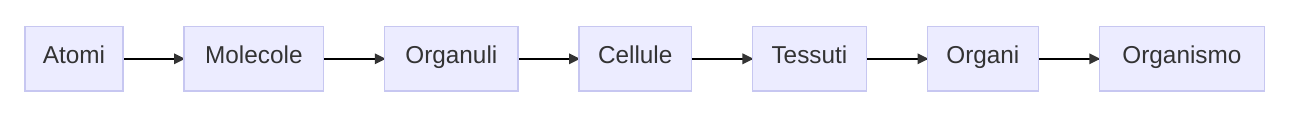
\includegraphics[scale=0.45] {images/strutture_biologiche.png}
\end{figure}


\par Tutta la materia è costituita da 94 elementi chimici in natura (tralasciando quelli non stabili). La materia organica è composta per il 96\% da atomi di C, O, N, H (carbonio, ossigeno, azoto, idrogeno). Un atomo ha un nucleo composto da neutroni e protoni circondato da una nube di elettroni in rapido movimento. Il Dalton (Da) è l'unità della massa atomica, corrisponde al peso di un protone o neutrone: $1 Da = 1.7 \times 10^{-24}g$. Un elettrone pesa $0.0005 Da$. Gli elettroni più esterni sono chiamati \textit{elettroni di valenza} e determinano il comportamento chimico di un atomo.

\par Lo scheletro dei composti organici è formato da catene carboniose, lunghe catene di atomi di carbonio legati fra loro da legami covalenti (il tipo di legame chimico più forte). Salendo di un livello nella gerarchia strutturale si arriva alle macromolecole biologiche, fondamentali per le cellule: carboidrati, lipidi, acidi nucleici e proteine. I carboidrati sono combustibili cellulari e materiale da costruzione, i lipidi sono sia depositi di energia che gusci protettivi, gli acidi nucleici permettono di codificare l'informazione genica e le proteine sono alla base delle funzioni vitali.\\

La cellula è la più piccola unità in grado di vivere. Per \textit{vivente} si intende un essere dotato di: organizzazione interna, metabolismo, omeostasi, interazione con l'ambiente, adattamento, crescita e riproduzione.

\par Le cellule hanno dimensioni che variano dai 2$\mu m$ ai $centimetri$ delle uova di rana, gallina o struzzo ai $metri$ di neuroni con lunghi assoni:

\begin{figure}[!h]
	\centering
	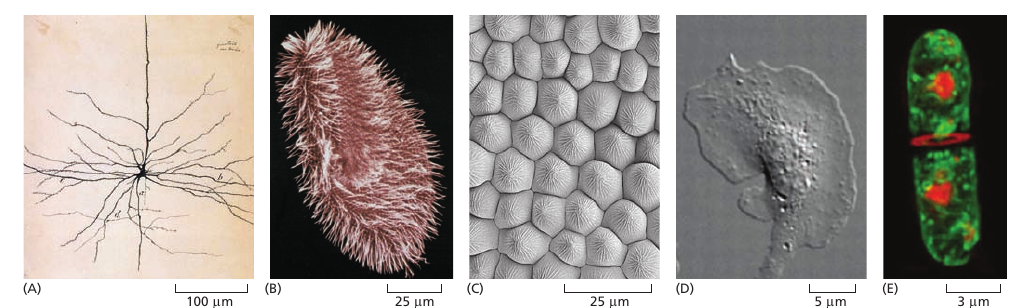
\includegraphics[scale=0.5] {images/cellule-dimensioni.png}
	\caption{(A) disegno di un neurone. (B) Paramecium. (C) superficie di un petalo di fiore di bocca di leone. (D) Macrofago. (E) Un lievito di fissione viene catturato nell'atto di divisione cellulare. Fonte: \cite{alberts2018essential}}
	\label{fig:cellule-dimensioni}
\end{figure}

\par È possibile dividere gli esseri viventi in due domini: \textit{procarioti} ed \textit{eucarioti}. Il primo include i due regni Bacteria e Archaea. Sono caratterizzati da cellule piccole, circa 1$\mu m$. Il secondo dominio include cinque regni: animali, piante, funghi, protisti e cromisti. Gli organismi eucarioti dispongono di cellule più grandi (circa 10-100 $\mu m$) dotate di compartimenti interni che dividono i processi cellulari.

La strutture tipiche di una cellula animale e di un neurone sono mostrate nelle seguenti figure:
\begin{figure}[!htb]
	\minipage{0.5\textwidth}
	\centering
	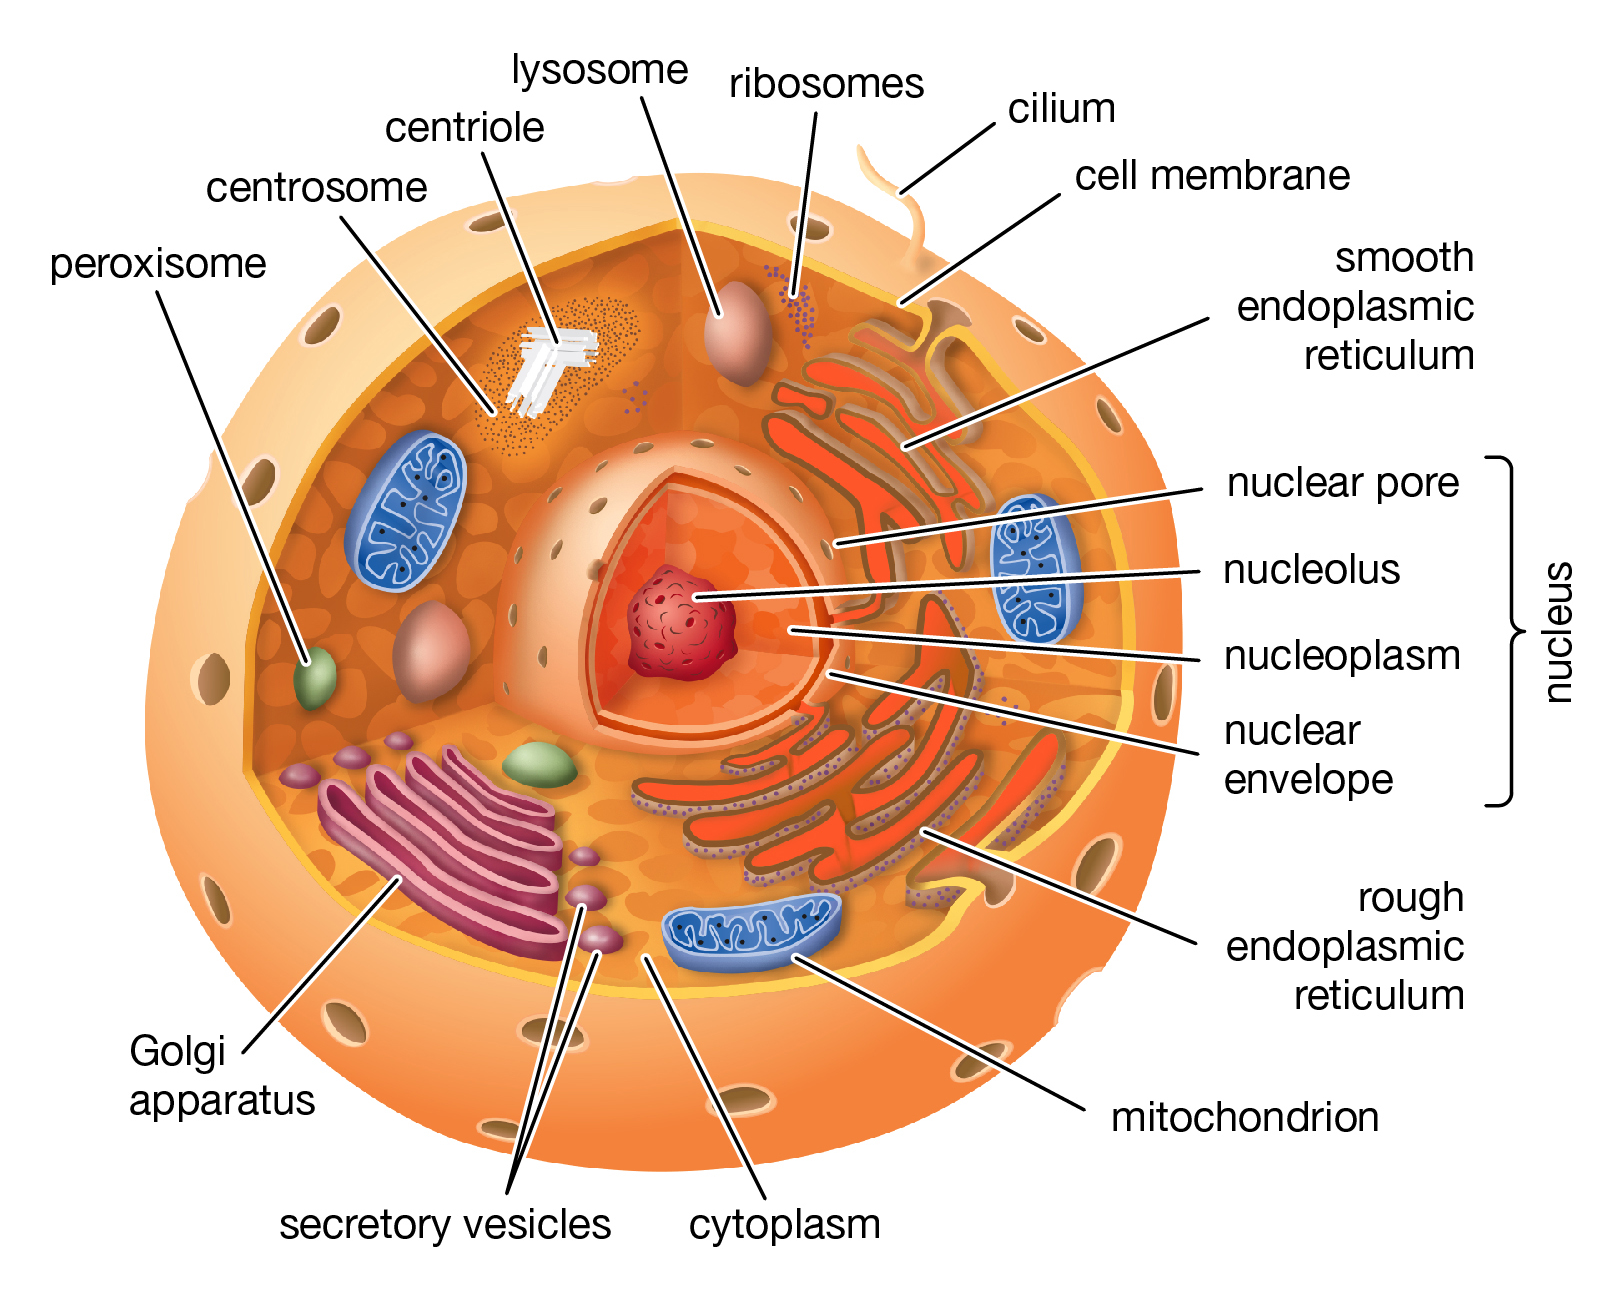
\includegraphics[scale=0.14]{images/cellula-eucariotica2.png}
	\caption{Cellula animale. Fonte: \cite{eukaryoteBritannica}}
	\label{fig:cellula-animale}
	\endminipage\hfill
	\minipage{0.5\textwidth}
	\centering
	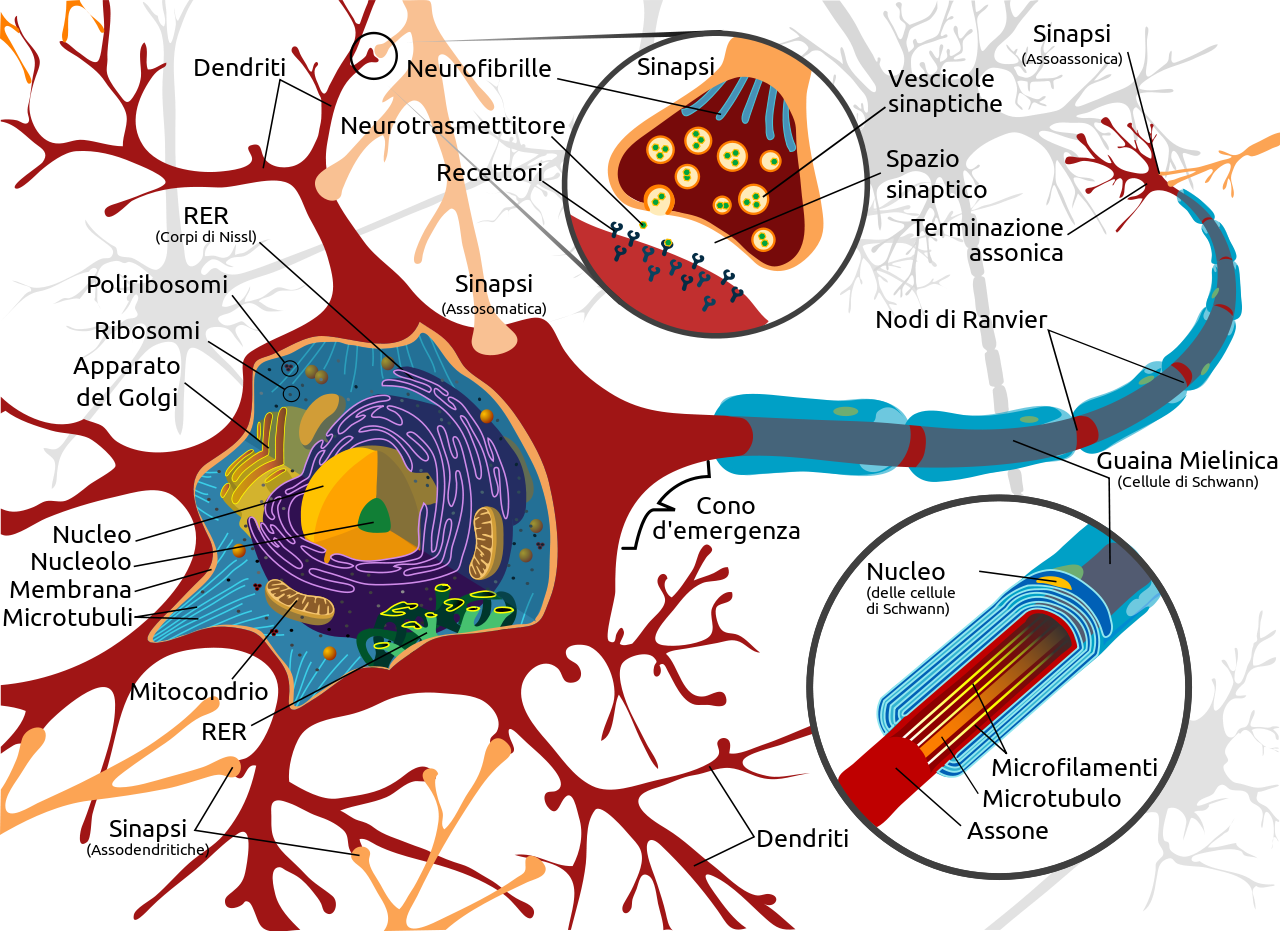
\includegraphics[scale=0.155]{images/neurone.png}
	\caption{Neurone. Fonte \cite{neuroneWiki}}
	\label{fig:neurone}
	\endminipage\hfill
\end{figure}

Una cellula eucariote animale è formata innanzitutto dalla membrana cellulare, un involucro costituito da un doppio strato fosfolipidico che permette alla cellula di avere il suo "spazio vitale" in quanto la separa dall'ambiente (spesso acquoso) circostante. È attraversata da piccoli pori che le permettono lo scambio di sostanze con l'esterno. Tutto ciò che si trova all'interno della cellula è immerso nel citoplasma, gel acquoso contenente grandi e piccole molecole. Il citosol è la parte del citoplasma non contenuta all'interno delle membrane intracelullari. Il volume totale delle cellule è composto da acqua per il 70\% circa. Vi è poi il citoscheletro che dà forma strutturale e permette movimenti direzionati. 

\par Il primo organello di grande importanza è il reticolo endoplasmatico, formato da tubuli e cisterne e in comunicazione con l'involucro nucleare. È rugoso quando sono presenti ribosomi (sintetizzatori di proteine). È il componente della fabbrica cellulare che si occupa di attività e sintesi di molecole fondamentali per la sopravvivenza della cellula (sintesi di steroidi, metabolismo del glucosio, eliminazione di sostanze nocive). L'apparato del Golgi produce vescicole che si fondono poi con la membrana cellulare: è una centrale di smistamento per confezionare sostanze da esportare. I lisosomi sono il centro di degradazione e riciclo della cellula. Il mitocondrio è la centrale energetica della cellula, dove avviene la respirazione cellulare: utilizza ossigeno per bruciare molecole organiche come zuccheri e grassi al fine di produrre energia che verrà immagazzinata sottoforma di ATP. 

\par Infine è presente il nucleo, custode del DNA. È formato dall'involucro nucleare, cromatina e nucleolo. Il DNA nel nucleo è associato a delle proteine con cui forma un materiale fibroso chiamato cromatina, mostrandosi "sfilacciato" in modo da poter essere letto. Quando la cellula si riproduce tali fibre si ispessiscono divenendo visibili come strutture compatte e singole: i cromosomi. Il nucleolo non è provvisto di membrana e serve per la sintesi di RNA ribosomiale, cioè l'RNA che uscendo dai pori dell'involucro nucleare andrà nel citoplasma a formare i ribosomi. Dall'involucro nucleare può uscire RNA e proteine ma non il DNA. \\

\par Il ciclo di vita delle cellule si basa su 4 fasi: crescita, sintesi del DNA, crescita completa e mitosi (divisione cellulare). Le cellule dei mammiferi impiegano da 18 a 24 ore per completare un ciclo di mitosi, mentre i lieviti solamente 90 minuti. Per questa ragione il lievito da fornaio (\textit{Saccharomyces cerevisiae}) è usato come organismo modello in citologia e genetica: il suo genoma è stato il primo ad essere sequenziato completamente tra gli eucarioti \supercite{lievitoWiki}. 

\par Le cellule hanno una durata di vita molto variabile, ad esempio alcuni organismi unicellulari come le spore possono vivere anche decenni, così come i nostri neuroni, mentre i globuli bianchi vengono ricambiati ogni 2 giorni. \\

\par Gli strumenti utilizzati per indagare nel mondo microscopico riescono a mostrare dettagli che vanno dal limite di 200$nm$ del microscopio ottico (limite imposto dalla natura ondulatoria della luce) alla precisione di 1$nm$ del microscopio a trasmissione elettronica (che usa fasci di elettroni invece di fasci di luce e necessita di campioni molto fini):

\begin{figure}[!h]
	\centering
	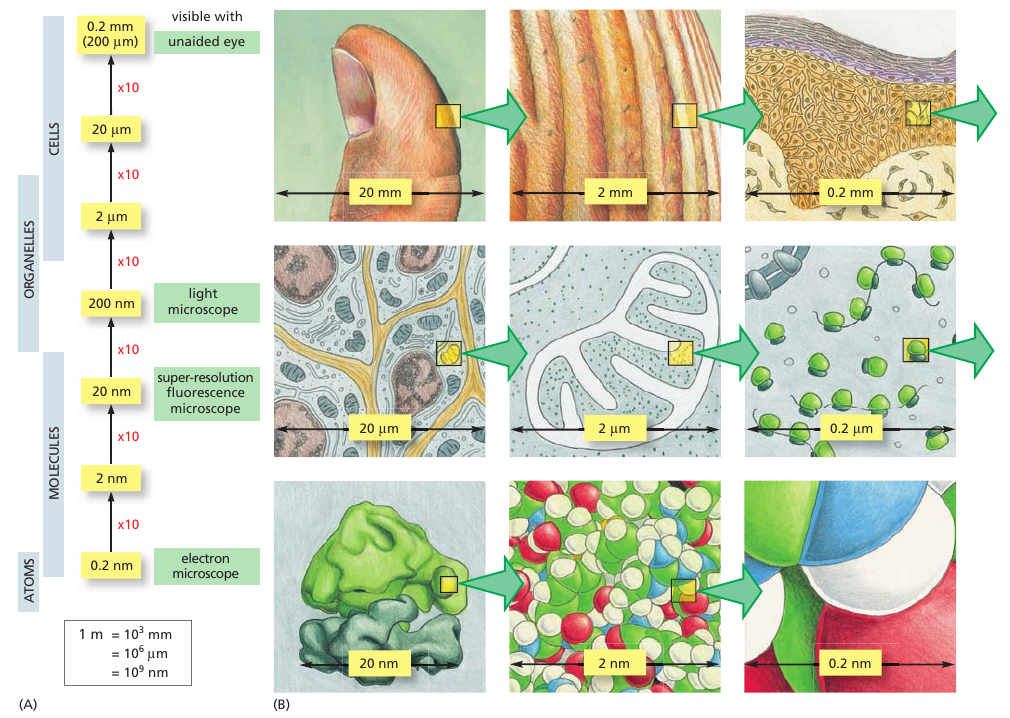
\includegraphics[scale=0.6]{images/grandezze.png}
	\caption{(A) Il grafico elenca le dimensioni dei livelli strutturali biologici, le unità di misura relative e gli strumenti necessari per visualizzarli. (B) Uno stesso dettaglio a varie scale di grandezza: pollice, pelle, cellule, mitocondrio, ribosomi, insieme di atomi che formano parte di una proteina. I dettagli molecolari sono oltre la potenza del microscopio elettronico. Fonte: \cite{alberts2018essential}}
	\label{fig:microscopi-grandezze}
\end{figure}

\subsection{Concetti fondamentali in biologia}

\begin{itemize}
	\item \textit{Proprietà emergenti }\\
			Ad ogni livello di indagine, ovvero passando da un livello della gerarchia strutturale al superiore, si palesano nuove proprietà non riconducibili ai livelli più semplici: le proprietà emergenti. Una singola molecola d'acqua non è né solida né liquida.
	\item \textit{Teoria cellulare} \\
			Le cellule rappresentano le unità strutturali e funzionali degli organismi.
	\item \textit{Geni} \\
			Il perpetuarsi della vita è possibile grazie alla trasmissione dei geni.
	\item \textit{Forma e funzione} \\
			Forma e funzione sono correlate a tutti i livelli biologici. Se le ali degli uccelli non fossero così come sono essi non potrebbero volare, se i mitocondri non avessero striature non potrebbero svolgere la respirazione cellulare, se i neuroni non avessero lunghi assoni non riuscirebbero a comunicare oppure si pensi al \textit{paramecium} che si muove come un sommergibile grazie alle sue ciglia (vedi figura \ref{fig:cellule-dimensioni}B).
	\item \textit{Evoluzione} \\
			L'evoluzione rappresenta il tema centrale ed unificante della biologia, come si è già accennato sopra. Gli organismi sono sistemi aperti che interagiscono continuamente con l'ambiente, dotati di variabilità individuale e finalizzati alla competizione per la sopravvivenza. 
	\item \textit{Diversità e unità} \\
			Vi sono da 5 a 30 milioni di specie differenti eppure scendendo sempre di più nella struttura degli organismi si osserva una similitudine quasi sconcertante. Un esempio che ci riguarda è la somiglianza fra le ciglia di \textit{paramecium} e le ciglia di una cellula epiteliale delle vie aeree degli esseri umani: presentano la stessa sezione trasversale. Il codice genetico (le triplette) sono universali, gli amminoacidi si condificano nello stesso modo per tutti gli organismi. Diversità e unità della vita sulla Terra sono due facce della stessa medaglia. Il sequenziamento dei genomi e il loro confronto, basato su approcci informatici, ha rivelato una conservazione evoluzionistica, un'eredità comune: è possibile infatti scambiare geni omologhi codificanti proteine del ciclo di divisione cellulare fra uomini e lievito \supercite{alberts2018essential}: una cellula di lievito ha quindi tutto il macchinario molecolare necessario per leggere e interpretare il nostro codice genetico e utilizzarlo per la produzione di proteine umane funzionanti. Sono osservazioni simili che hanno guidato la direzione di alcune tecniche informatiche, anche per la predizione della struttura di proteine (come si vedrà successivamente).
			
\end{itemize}

\subsection{Dogma centrale della biologia}

Nel 1958 il premio Nobel Francis Crick introdusse il \textit{dogma} centrale della biologia, che allo stato attuale si può considerare come l'insieme dei principali meccanismi alla base dell'espressione genica. 

\begin{figure}[h]
	\centering
	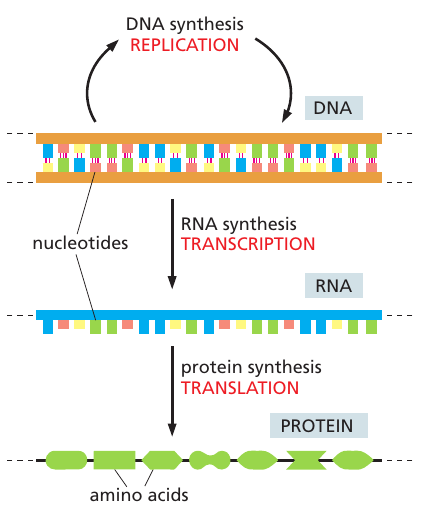
\includegraphics[scale=0.45]{images/central-dogma.png}
	\caption{Dogma centrale in biologia. Fonte \cite{alberts2018essential}}
	\label{fig:central-dogma}
\end{figure}

Il dogma descrive il flusso di informazione genetica: essa è conservata negli acidi nucleici DNA (RNA per alcuni virus) che possono essere duplicati, il DNA viene poi trascritto sottoforma di RNA e se codificante questo è poi tradotto in proteine, concepite come la forma operativa e terminale delle informazioni contenute nel genoma \supercite{dogma-wiki}.

\par Per avere una miglior panoramica del funzionamento di questo principio è importante approfondire la struttura del DNA (\textit{acido desossiribonucleico}). Il DNA è una molecola composta da due catene complementari che si avvolgono l'una intorno all'altra tramite legami idrogeno formando una doppia elica. Le catene sono chiamate filamenti e sono antiparalleli. Dal punto di vista chimico è un polimero di nucleotidi, dove ogni nucleotide è composto da una base azotata, uno zucchero pentoso (\textit{ribosio} nell'RNA e \textit{desossiribosio} nel DNA) e un gruppo fosfato (vedi figura \ref{fig:nucleotide}). Per ogni giro dell'elica vi sono 10 coppie di basi. La struttura a doppia elica consente un'agevole meccanismo di replicazione del DNA, coadiuvato dagli enzimi DNA polimerasi, primasi e DNA ligasi. Gli accoppiamenti seguono delle regole precise: GC, AT/AU, da una parte deve esserci una pirimidina (C, T) e dall'altra una purina (A,G):

\begin{figure}[!htb]
	\minipage{0.6\textwidth}
	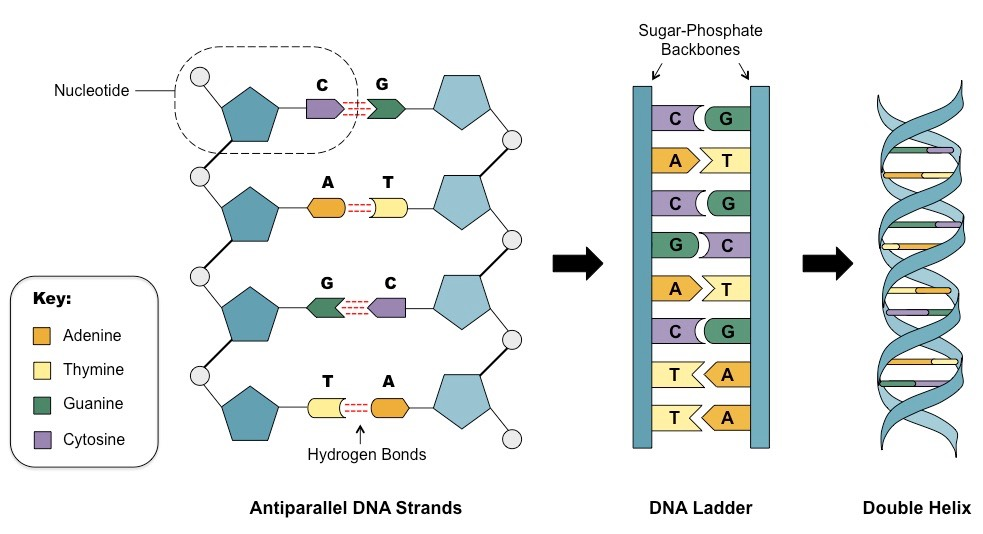
\includegraphics[scale=0.25]{images/double-stranded-dna_med.jpeg}
	\caption{struttura del DNA. Fonte: \cite{dna-image}}
	\label{fig:dna}
	\endminipage\hfill
	\minipage{0.4\textwidth}
	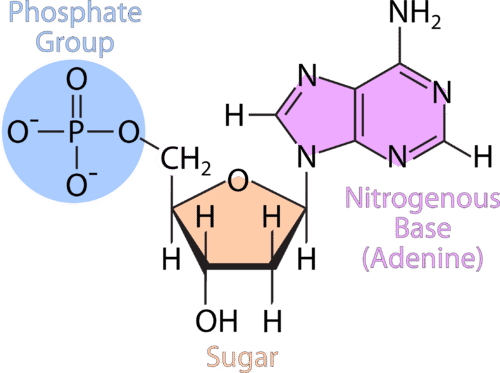
\includegraphics[scale=0.3]{images/nucleotide.png}
	\caption{Componenti di un nucleotide con Adenina per base azotata. Fonte \cite{introChimicaLibreTexts}}
	\label{fig:nucleotide}
	\endminipage\hfill
\end{figure}

Il \textit{genoma} indica il patrimonio complessivo del DNA di una cellula. Lo stesso gene nella stessa specie può esistere in varie forme, con leggere differenze nella sequenza nucleotidica: si sta parlando dei differenti \textit{alleli} del gene.
Gli alleli di tutti i geni di un individuo determinano il suo \textit{genotipo}.  Il \textit{fenotipo} indica invece l'insieme delle caratteristiche morfologiche e funzionali di un organismo, quali risultano dall'espressione del suo genotipo e dalle influenze ambientali. In un organismo, nonostante tutte le cellule condividano gli stessi geni, cellule afferenti a organi o tessuti diversi esprimono geni differenti (\textit{espressione genica}).
\\

\par L'RNA (\textit{acido ribonucleico}) esiste in varie forme. Le differenze con il DNA sono mostrate nella figura \ref{fig:rna-dna-differenze}, si può notare che vi è un singolo filamento e che la base azotata timina è assente e al suo posto si trova la base uracile (U). Essendo ad un unico filamento può formare legami a idrogeno con sé stessa e assumere forme tridimensionali vantaggiose. Esistono vari tipi di RNA: 

\begin{itemize}
	\item mRNA, messaggero, contiene l'informazione per la sintesi delle proteine
	\item tRNA, di trasporto, necessario per la traduzione nei ribosomi
	\item rRNA, ribosomiale, entra nella struttura dei ribosomi
	\item RNA catalitico o ribozima, enzima ad RNA, è una molecola di RNA in grado di catalizzare una reazione chimica similmente agli enzimi
	\item snRNA, hnRNA
\end{itemize}

\begin{figure}[h]
	\centering
	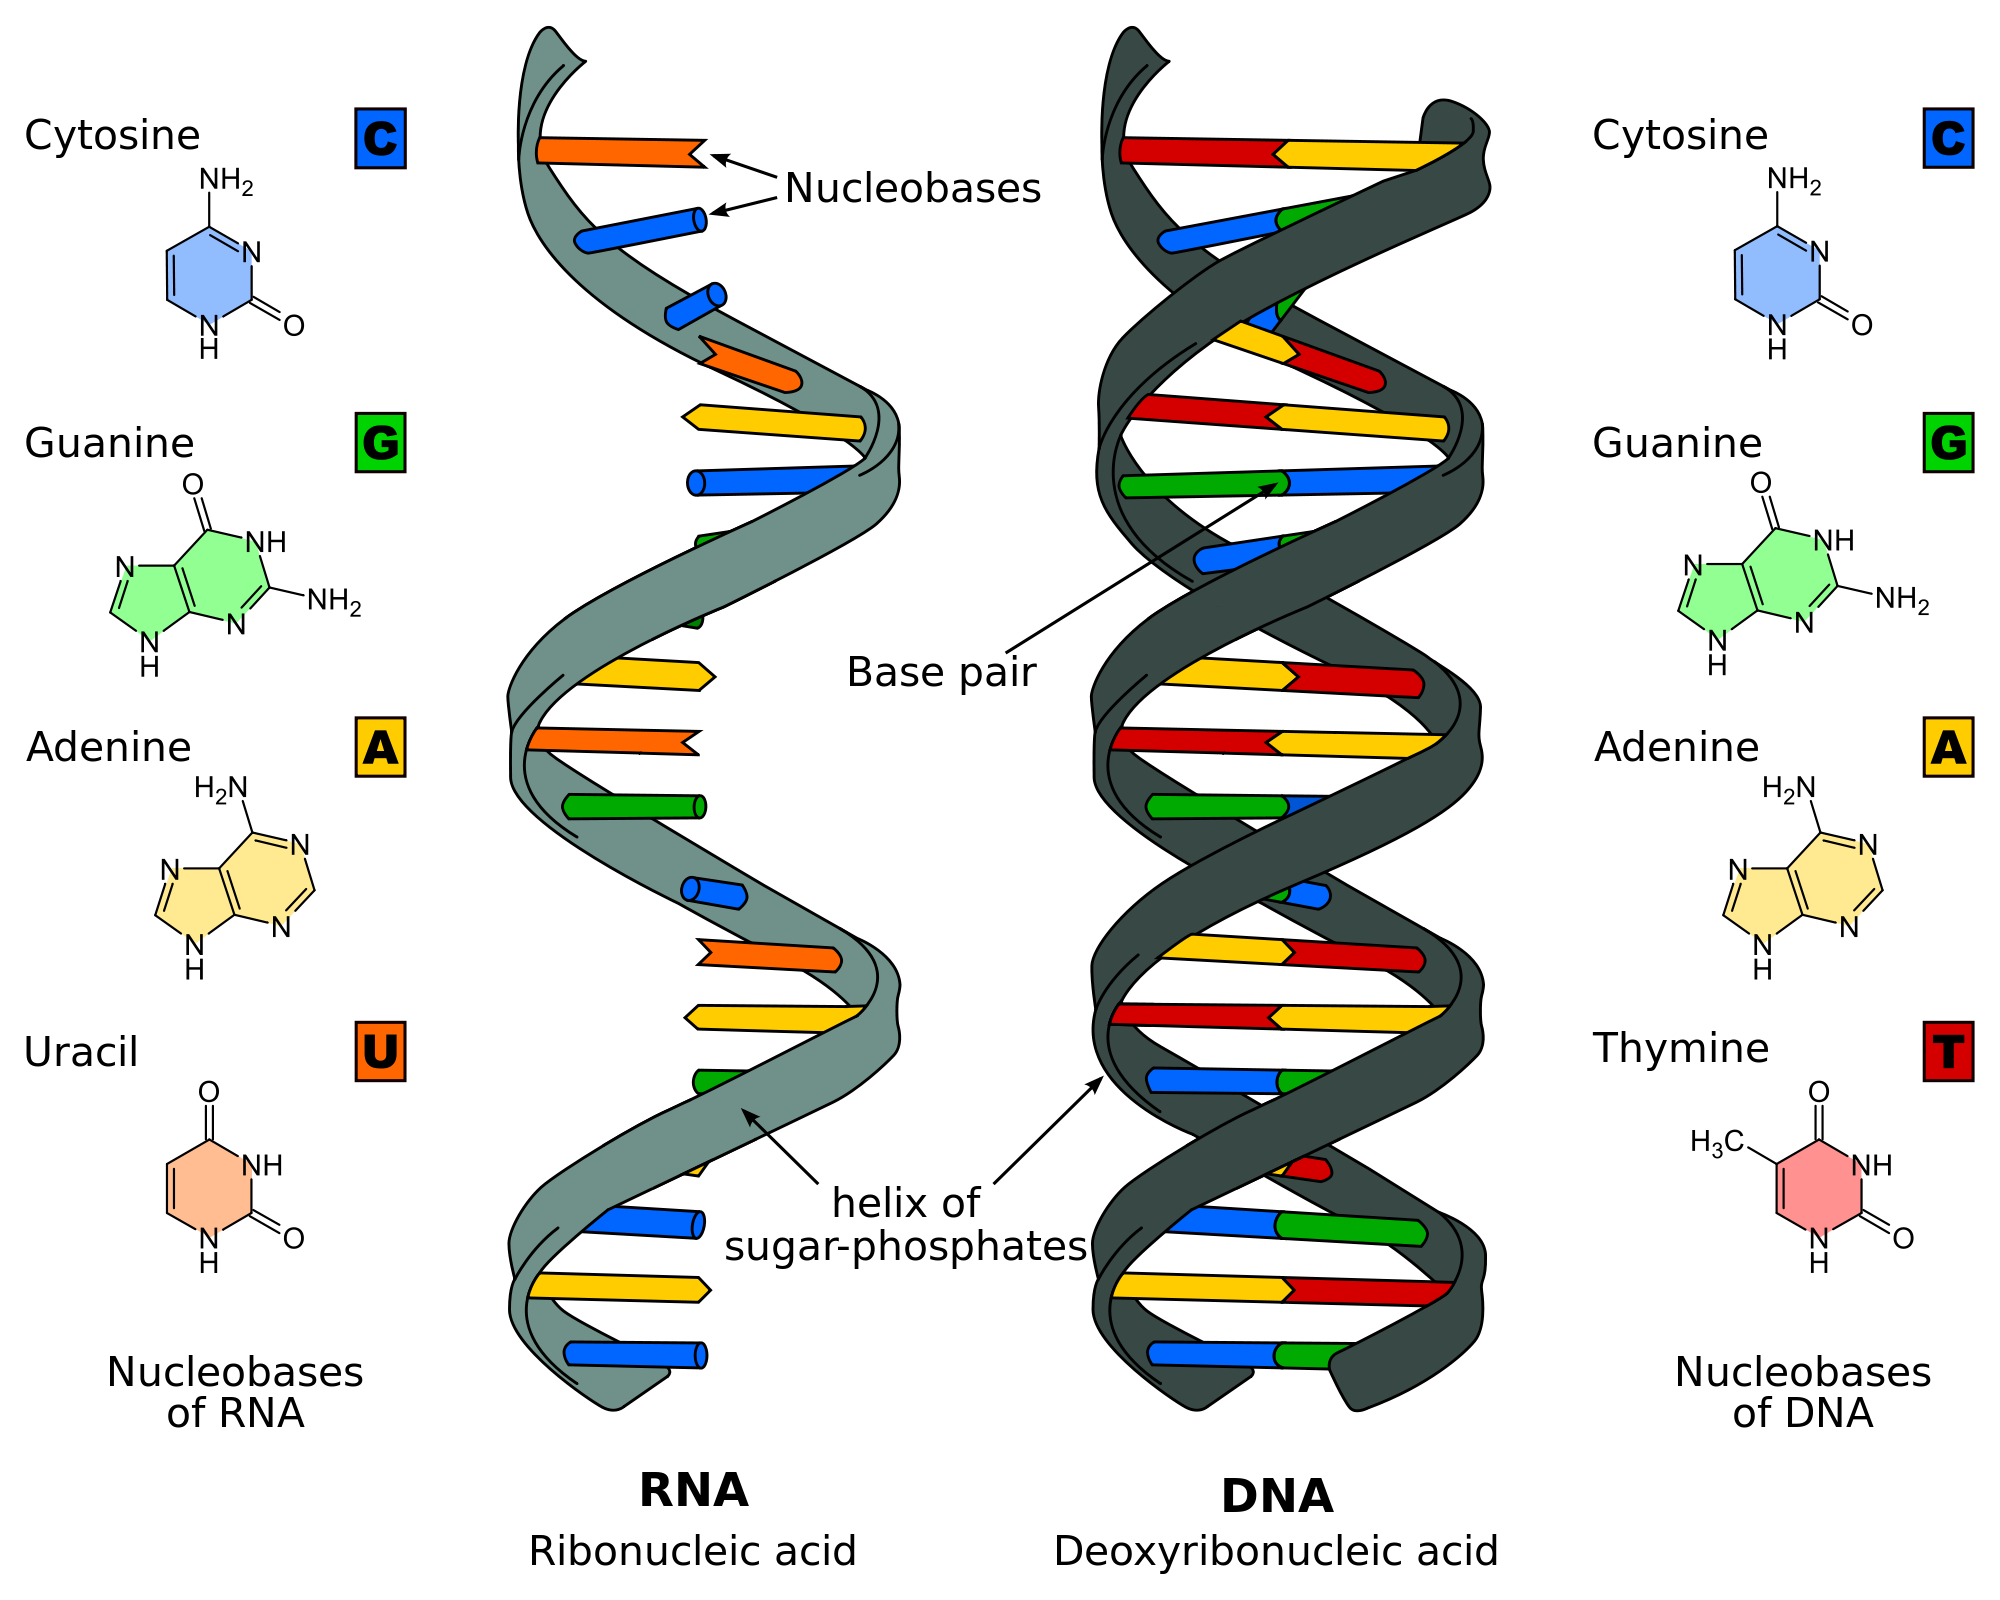
\includegraphics[scale=0.15]{images/dna-rna.png}
	\caption{Differenze fra RNA e DNA Fonte: \cite{dna-rna-image}}
	\label{fig:rna-dna-differenze}
\end{figure}

Il DNA dell'uomo contiene $3\time10^{9}$ coppie di nucleotidi, contenente circa $21000$ geni codificanti: se il genoma umano venisse esteso in lunghezza sarebbe lungo 2,2 metri. Il batterio più semplice contiene 500 geni codificanti mentre il genoma di un'ameba è 100 volte più lungo di quello umano \supercite{alberts2018essential}, tanto per avere una visione quantitativa della diversità genetica tra gli organismi.


\subsection{Dai geni alle proteine}

Il codice genetico lavora a sequenze di codici di 3 lettere (es. "GAA" = Glutammato), questo perché si hanno a disposizione 4 lettere (le basi azotate) e si devono codificare i 20 diversi amminoacidi. Con 2 lettere avrei $4^{2}$ possibilità che non sono sufficienti a descrivere 20 informazioni diverse, si utilizzano pertanto 3 lettere anche se ciò causa ridondanza nei codici. Un amminoacido è quindi codificato da una tripletta: si parla di \textit{codice a triplette}. \\

\par Il primo passo consiste nella \textit{trascrizione}. Un filamento di DNA fa da stampo per la creazione di mRNA, il tutto esclusivamente tramite \textit{complementarità di forma}. Il DNA non viene aperto come una zip ma l'apertura, la trascrizione (compiuta dall'RNA polimerasi, soggetta a errori anche frequenti) e la chiusura della doppia elica avvengono di pari passo. Vi è un terminatore nel DNA per indicare la fine del gene. 

\par Le triplette nucleotidiche dell'mRNA sono dette \textit{codoni} e codificano un amminoacido. I codoni devono essere letti in direzione 5' -> 3'. La molecola di mRNA lascia il nucleo attraverso i pori nucleari. È importante osservare che non tutti i geni codificano proteine (lo stadio di trascrizione potrebbe risultare quello finale) e che il codice genetico è \textit{universale}, è condiviso dai batteri, piante, animali: per tutti la prolina si codifica in "CCG".

\par Negli eucarioti è presente un passaggio intermedio: la \textit{maturazione}, o fase di processamento. È composto da due sottofasi:
\begin{itemize}
	\item \textit{incapsulamento}, viene aggiunta una coda e un cappuccio alle due estremità al fine di proteggere l'mRNA dalla degradazione e per segnalare l'inizio ai ribosomi.
	\item \textit{splicing}, il DNA possiede lunghe sequenze nucleotidiche non codificanti, gli \textit{introni}. In questa fase vengono rimossi e gli \textit{esoni} (sequenze codificanti) vengono riunite insieme. È in questa fase che è possibile dare origini a sequenze primarie (delle proteine) diverse a partire da un unico gene.
\end{itemize}

\par L'ultimo passaggio è la \textit{traduzione}, attraverso la quale la cellula interpreta il messaggio genetico e polimerizza gli amminoacidi per costruire la relativa proteina. Il processo di traduzione è la transizione da un linguaggio a 4 lettere (basi azotate) ad un linguaggio a 20 lettere (amminoacidi). La traduzione viene realizzata dal tRNA, una sorta di adattatore da linguaggio \textit{genetico }a linguaggio \textit{amminoacidico}. Il tRNA è un acido nucleico a forma di L composto da circa 80 basi, da un'estremità vi è l'anticodone (interfaccia con il linguaggio genetico) e dall'altra vi è il sito di legame con un singolo amminoacido. Il tRNA trasporta ai ribosomi uno specifico amminoacido contenuto nel citoplasma. Esiste di conseguenza uno specifico tipo di tRNA per ogni codone.

\begin{figure}[!htb]
	\minipage{0.5\textwidth}
	\centering
	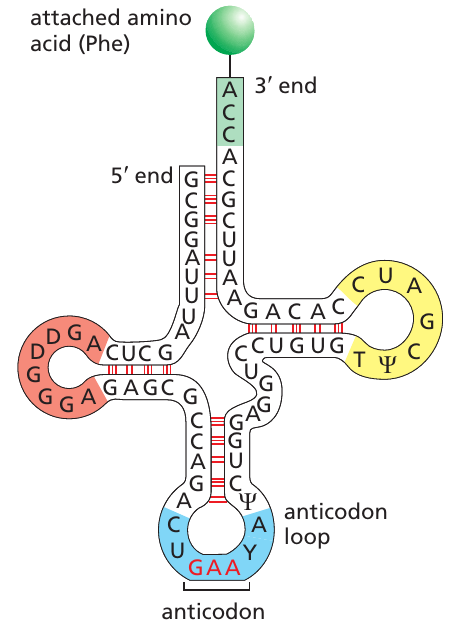
\includegraphics[scale=0.32]{images/tRNA.png}
	\caption{tRNA. Fonte \cite{alberts2018essential}}
	\label{fig:tRNA}
	\endminipage\hfill
	\minipage{0.5\textwidth}
	\centering
	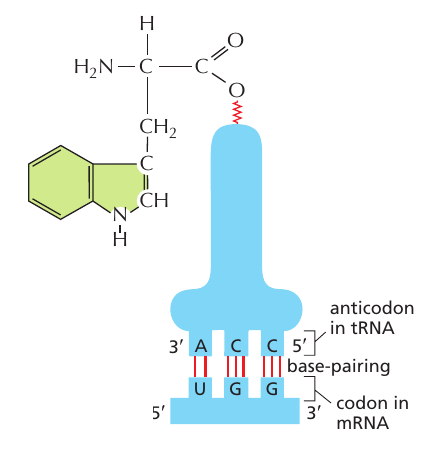
\includegraphics[scale=0.45]{images/tRNA-legame-traduzione.png}
	\caption{Traduzione: l'amminoacido triptofano (Trp) è codificato dal codone UGG nell'mRNA e si lega al tRNA tramite un legame energetico forte. Fonte: \cite{alberts2018essential}}
	\label{fig:tRNA-legame}
	\endminipage\hfill
\end{figure}

\par È interessante notare che il tRNA, proprio come le proteine, è caratterizzato dall'avere più strutture: quella primaria, costituita dalla sua sequenza nucleotidica, quella secondaria data dalla sua struttura a quadrifoglio e quella terziaria dovuta alla struttura tridimensionale a L. La differenza fra la struttura del tRNA e delle proteine sono gli elementi unitari: nel tRNA si tratta di nucleotidi mentre nelle proteine di amminoacidi.

\begin{figure}[h]
	\centering
	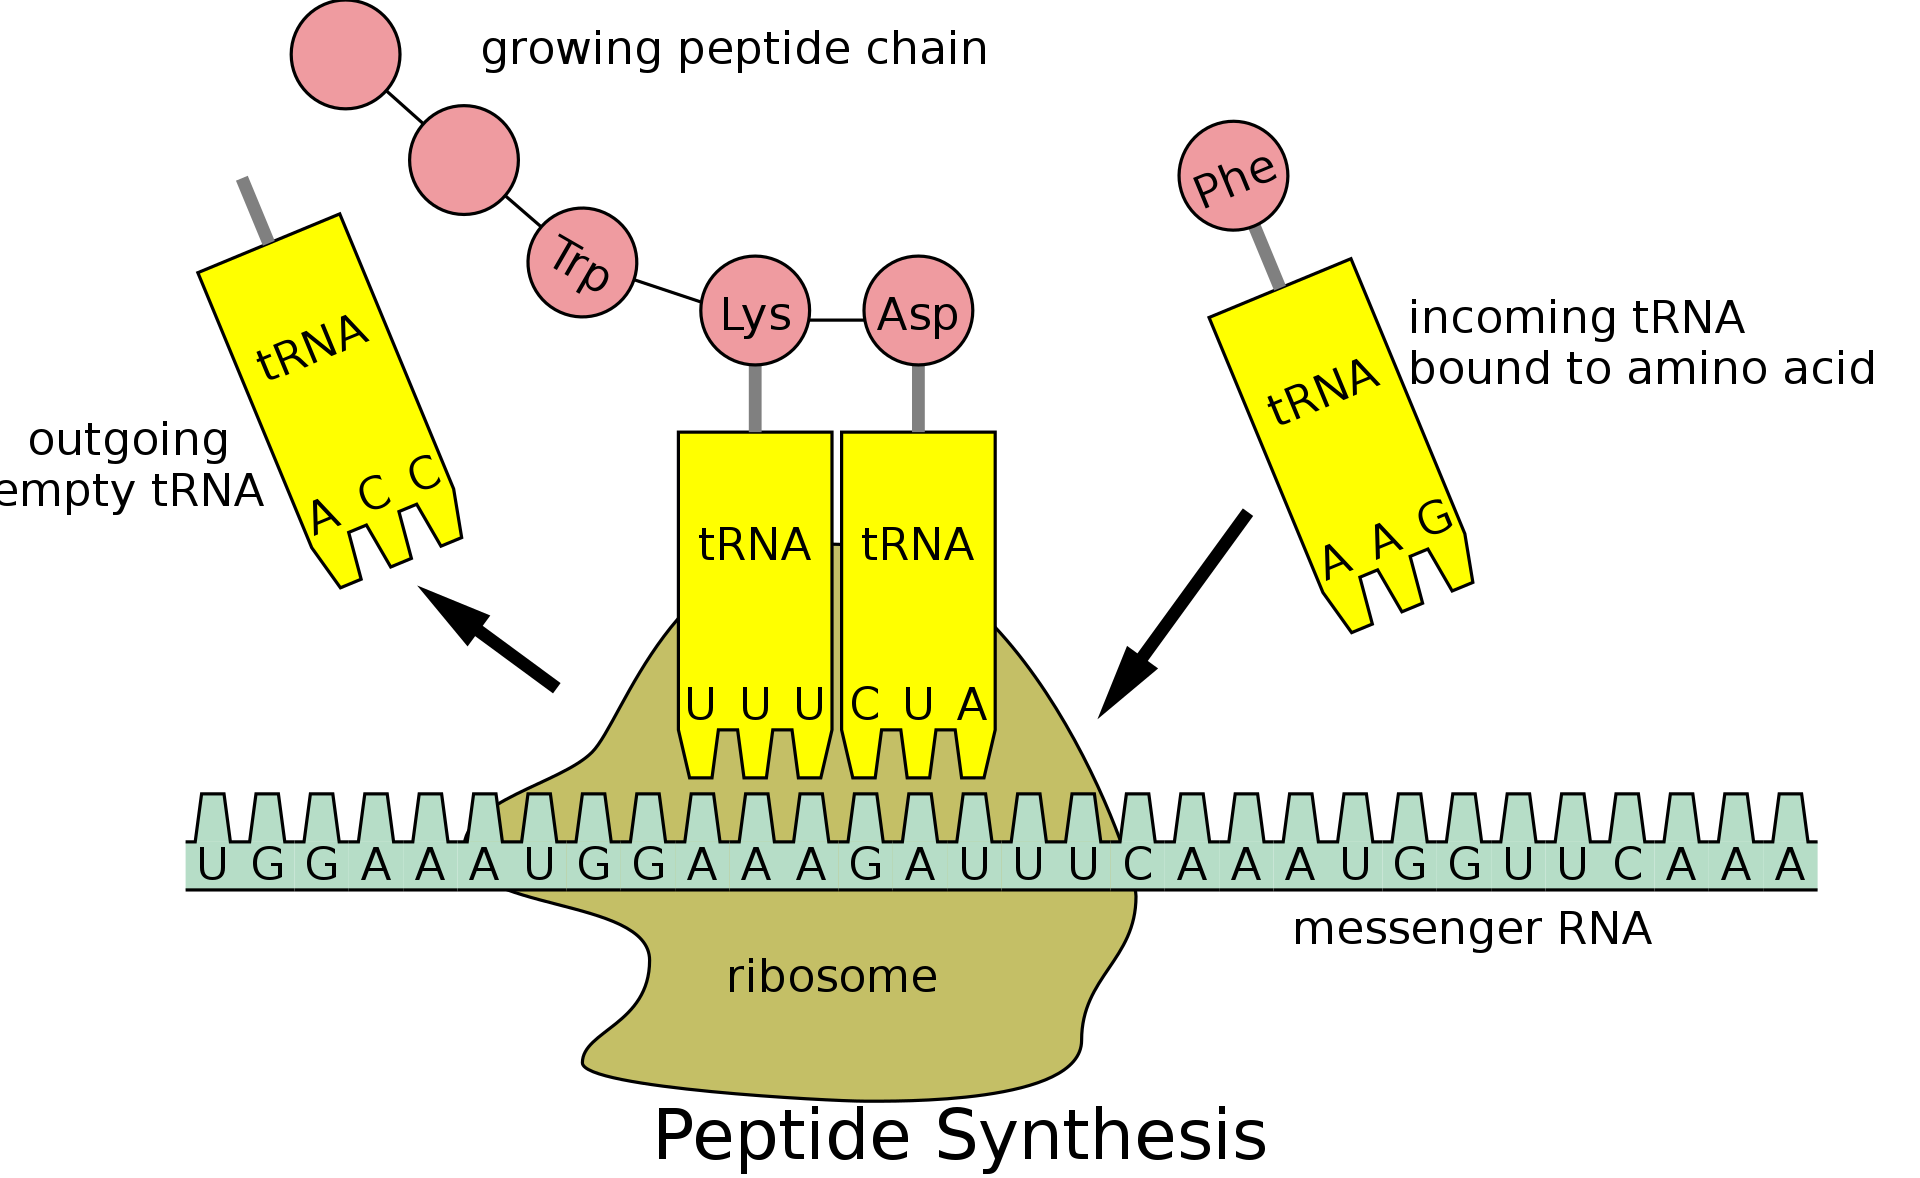
\includegraphics[scale=0.15]{images/traduzione.png}
	\caption{Traduzione, sintesi peptidica. Fonte: \cite{tRNAwiki}}
	\label{fig:traduzione}
\end{figure}

La traduzione comincia con il primo codone (AUG, che oltre a segnalare l'inizio codifica anche la metionina, vedi figura \ref{fig:codici-amminoacidi}) al quale si incastra nel ribosoma un tRNA avente il corrispondente amminoacido legato. Si formano legami idrogeno fra i nucleotidi. Arriva un secondo tRNA combaciante con il successivo codone. I due amminoacidi si trovano vicini e formano un legame peptidico. L'mRNA scorre così che si crei posto per nuovi tRNA, nel frattempo gli amminoacidi si legano fra loro e cominciano a formare la proteina. Il ripiegamento della proteina comincia già durante la sua biosintesi. Il processo termina quando si arriva ad un codone di stop (es. UAA). Per velocizzare il processo di sintesi ribosomiale questo viene parallelizzato: tanti \textit{poliribosomi} sono associati allo stesso mRNA attuando una rapida sintesi di copie multiple di un polipeptide a partire da un unico mRNA.

\begin{figure}[h]
	\centering
	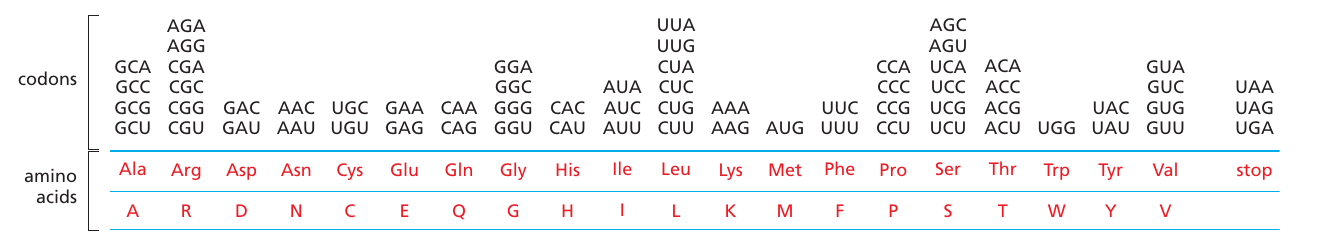
\includegraphics[scale=0.46]{images/codici-amminoacidi.png}
	\caption{Codici a tripletta degli amminoacidi. Fonte: \cite{alberts2018essential}}
	\label{fig:codici-amminoacidi}
\end{figure}

\subsection{Proteine: le macromolecole più importanti della vita}

Le proteine sono formate dall'unione di strutture più semplici: gli amminoacidi. Un polimero amminoacidico composto da meno di 50 amminoacidi è chiamato \textit{peptide}, se supera tale soglia \textit{polipeptide}. Una proteina può essere quindi sia un semplice peptide \footnote{Esempi di "semplici" peptidi che svolgono funzioni biologiche sono i \textit{neuropeptidi} che agiscono da neurotrasmettitore (ad es. endorfine) e \textit{ormoni} quali l'insulina e il glucagone} che un singolo polipeptide o essere formata da più polipeptidi. La sequenza amminoacidica determina la struttura della proteina ed è proprio questo il collegamento fra il messaggio genetico nel DNA e la struttura tridimensionale che è associata alla sua funzione biologica. 

\par Un amminoacido è una molecola organica formata da un atomo di carbonio centrale chiamato $C_{\alpha}$ circondato da 4 componenti (vedi fig. \ref{fig:amminoacido}):
\begin{enumerate}
	\item un atomo di idrogeno
	\item un gruppo amminico ($\alpha-amino$), (-NH$_{2}$) in condizioni fisiologiche carico positivamente (-NH$_{3}^{+}$) 
	\item un gruppo carbossilico ($\alpha-carboxyl$), (-COOH) carico negativamente (-COO$^{-}$)
	\item un gruppo R, gruppo laterale chiamato anche \textit{residuo} che per sineddoche indica l'intero amminoacido una volta che questo si trova all'interno della catena proteica
\end{enumerate}

Vi sono circa 20 amminoacidi proteinogenici diversi (come si può vedere nella figura \ref{fig:codici-amminoacidi} o \ref{fig:amminoacidi-tipi}). Il gruppo laterale non partecipa alla catena della \textit{backbone} (spina dorsale) della proteina, resa stabile dai legami peptidici: rimane infatti libero di legarsi. È questo il "trucco" che consente alla proteina sia di ripiegarsi su sé stessa che di legarsi ad altre molecole. Gli amminoacidi possono essere polari, non polari, carichi (vedi figura \ref{fig:amminoacidi-tipi}) e causano differenti ripiegamenti della proteina. Di conseguenza ne influenzano la funzione, si pensi infatti al caso dell'anemia falciforme causata da 1 solo amminoacido di differenza: valina al posto del glutammato. La prima non è polare mentre il secondo è polare carico, ciò causa legami differenti, quindi ripiegamento differente e funzione biologica compromessa. 

\par Gli amminoacidi esistono in 2 configurazioni: L e D. Essi sono infatti molecole \textit{chirali}: le due configurazioni sono l'immagine speculare l'una dell'altra ma non sono sovrapponibili. Nella grande maggioranza degli organismi viventi le proteine sono composte solo da amminoacidi della serie L.

\begin{figure}[!htb]
	\minipage{0.45\textwidth}
	\centering
	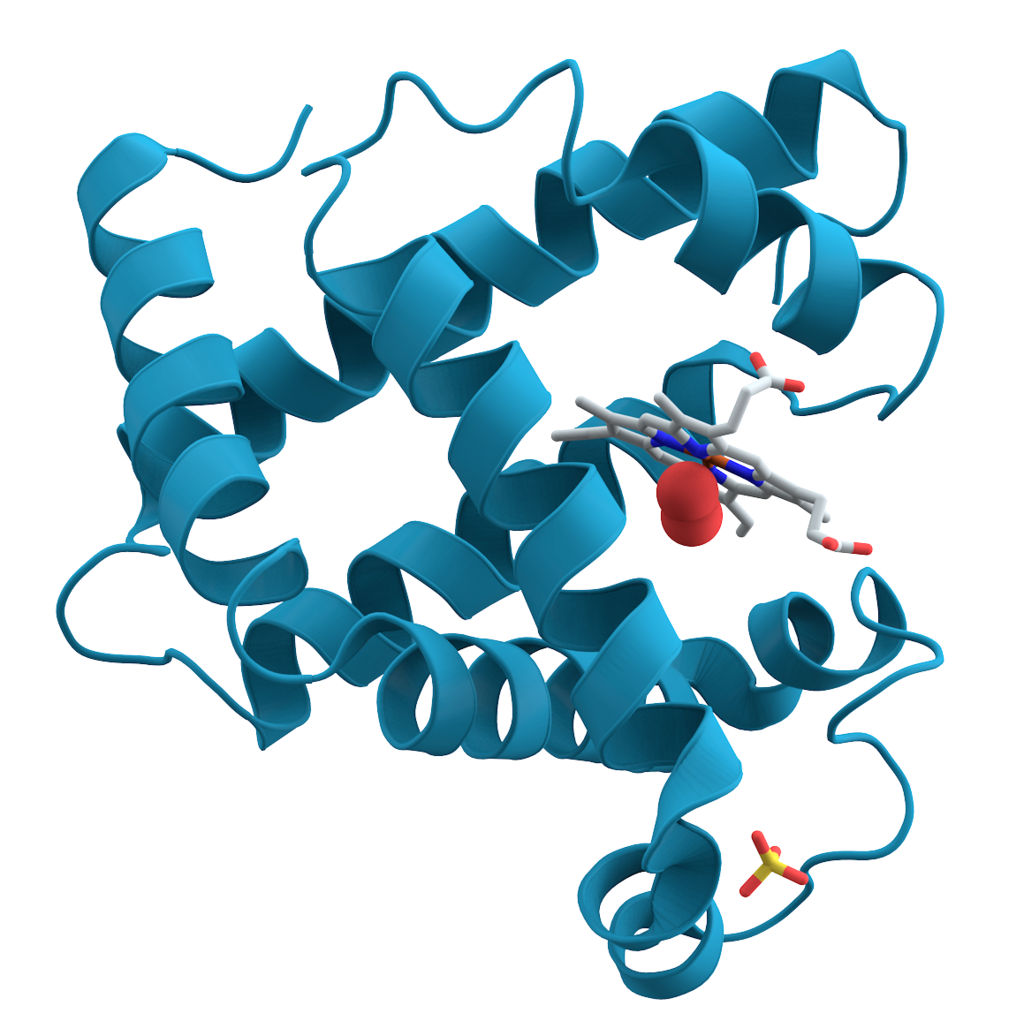
\includegraphics[scale=0.15]{images/mioglobina.png}
	\caption{Rappresentazione a nastro della struttura tridimensionale della mioglobina. È presente un gruppo hemo al quale è legata una molecola di ossigeno (rossa). Fonte: \cite{proteinWiki}}
	\label{fig:mioglobina}
	\endminipage\hfill
	\minipage{0.5\textwidth}
	\centering
	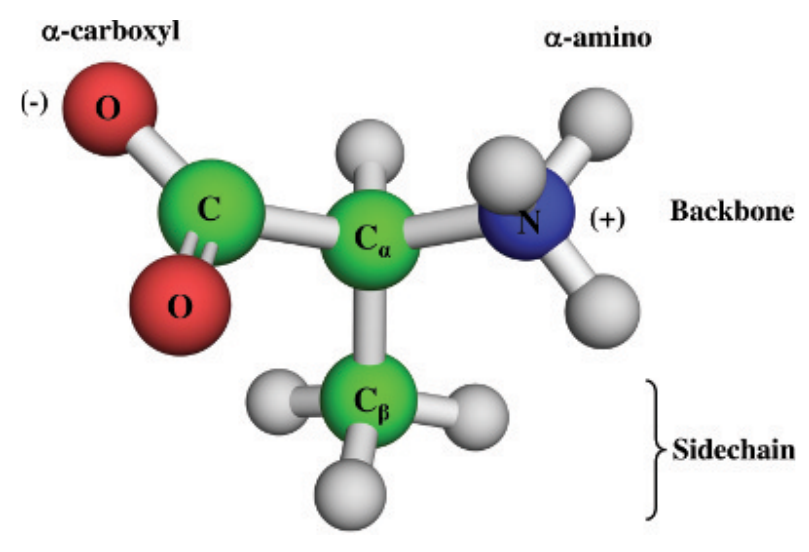
\includegraphics[scale=0.3]{images/amminoacido.png}
	\caption{Struttura principale degli amminoacidi. Fonte \cite{kessel_ben-tal_2018}}
	\label{fig:amminoacido}
	\endminipage\hfill
\end{figure}

\par Il legame peptidico è il legame che unisce tutti gli amminoacidi di una proteina: unisce il gruppo carbossilico di un amminoacido al gruppo amminico di un altro amminoacido. È un tipo di legame molto stabile, infatti l'emivita della backbone è di 400 anni a 25°C \supercite{alberts2018essential}. Il legame peptidico comporta l'eliminazione della carica degli ex gruppi \textit{amminico} e \textit{carbossilico}. 

\begin{figure}[!htb]
	\minipage{0.5\textwidth}
	\centering
	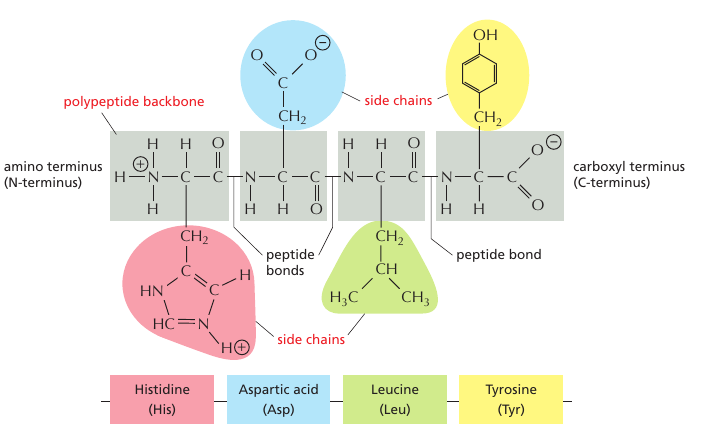
\includegraphics[scale=0.43]{images/protein-backbone.png}
	\caption{Backbone delle proteine. Fonte: \cite{alberts2018essential}}
	\label{fig:backbone}
	\endminipage\hfill
	\minipage{0.5\textwidth}
	\centering
	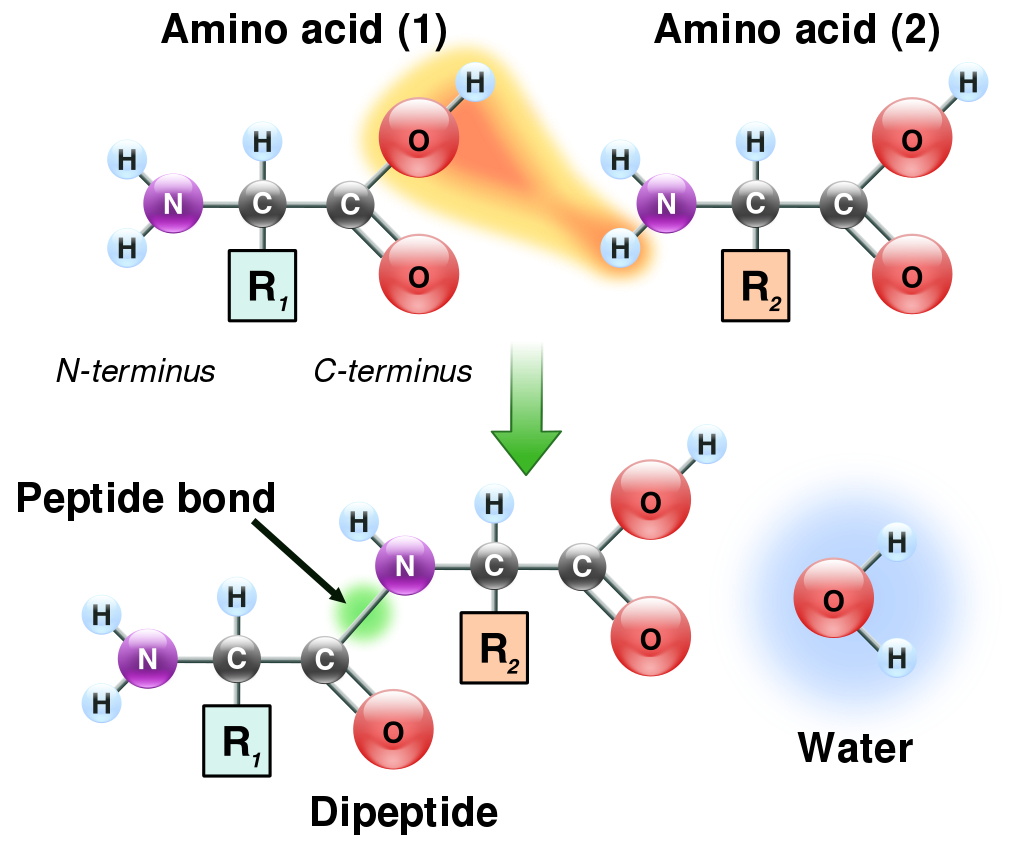
\includegraphics[scale=0.18]{images/peptide-bond.png}
	\caption{Legame peptidico. Fonte \cite{peptideBondWiki}}
	\label{fig:legame-peptidico}
	\endminipage\hfill
\end{figure}

Gli unici due residui elettricamente carichi rimasti in una proteina sono quelli alle due estremità (C-terminus ed N-terminus, vedi fig. \ref{fig:backbone}). È presente però un fenomeno che permette ai residui di interagire elettrostaticamente: la \textit{risonanza elettronica}. Gli elettroni dei legami possono estendersi su più atomi e permettere al residuo di assumere diverse configurazioni elettroniche. \\

\par Le proteine sono una classe di macromolecole con funzioni biologiche vitali, consentono infatti il funzionamento di ogni sistema vivente. Riusciamo a pensare, parlare, a digerire il cibo, a muoverci grazie alle proteine. Sono la base della vita cellulare e molecolare. 

\par Un tipo fondamantale di proteine sono gli enzimi, come accennato inizialmente. Una loro funzione importante è correlata alla digestione negli animali. Enzimi come le \textit{amilasi} e le \textit{proteasi }sono in grado di ridurre le macromolecole (nella fattispecie amido e proteine) in unità semplici (maltosio e amminoacidi), assorbibili dall'intestino.

\par Oltre agli enzimi ci sono tante altre proteine importanti. Uno degli esempi più noti è l'emoglobina, proteina animale adibita a trasportare ossigeno dai polmoni agli organi e ai tessuti del corpo così come a riportare CO$_{2}$ ai polmoni. Una molecola di emoglobina è composta da 4 polipeptidi e contiene 4 atomi di ferro che le consentono di legare reversibilmente 4 molecole di ossigeno.

\begin{figure}[!htb]
	\minipage{0.45\textwidth}
	\centering
	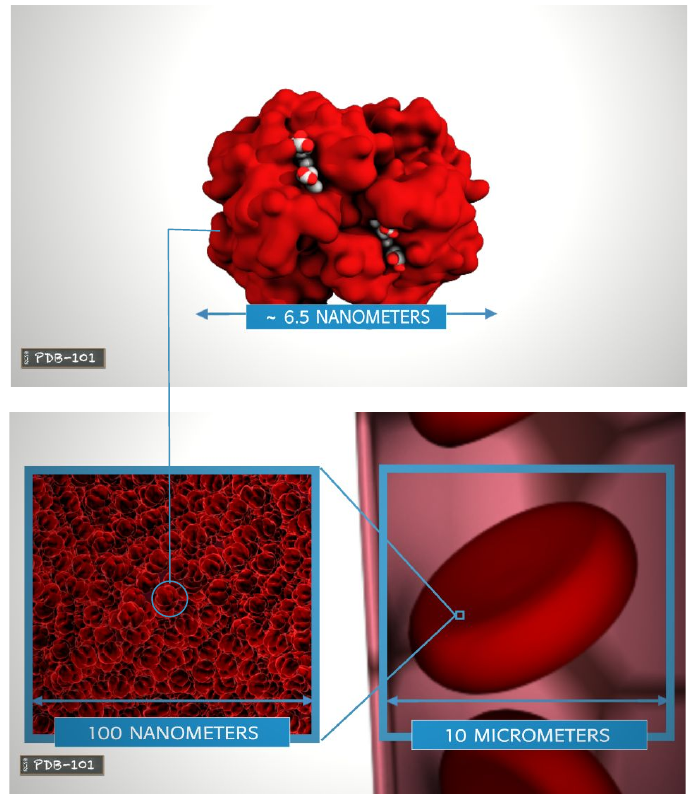
\includegraphics[scale=0.38]{images/emoglobina-dimensioni.png}
	\caption{Emoglobina in diverse scale. Rappresentazione a superficie. Un globulo rosso contiene circa 280 milioni di molecole di emoglobina, per cui può portare più di 1 miliardo di molecole di ossigeno per volta. Fonte: \cite{ProteinRCSB}}
	\label{fig:emoglobina-dimensioni}
	\endminipage\hfill
	\minipage{0.5\textwidth}
	\centering
	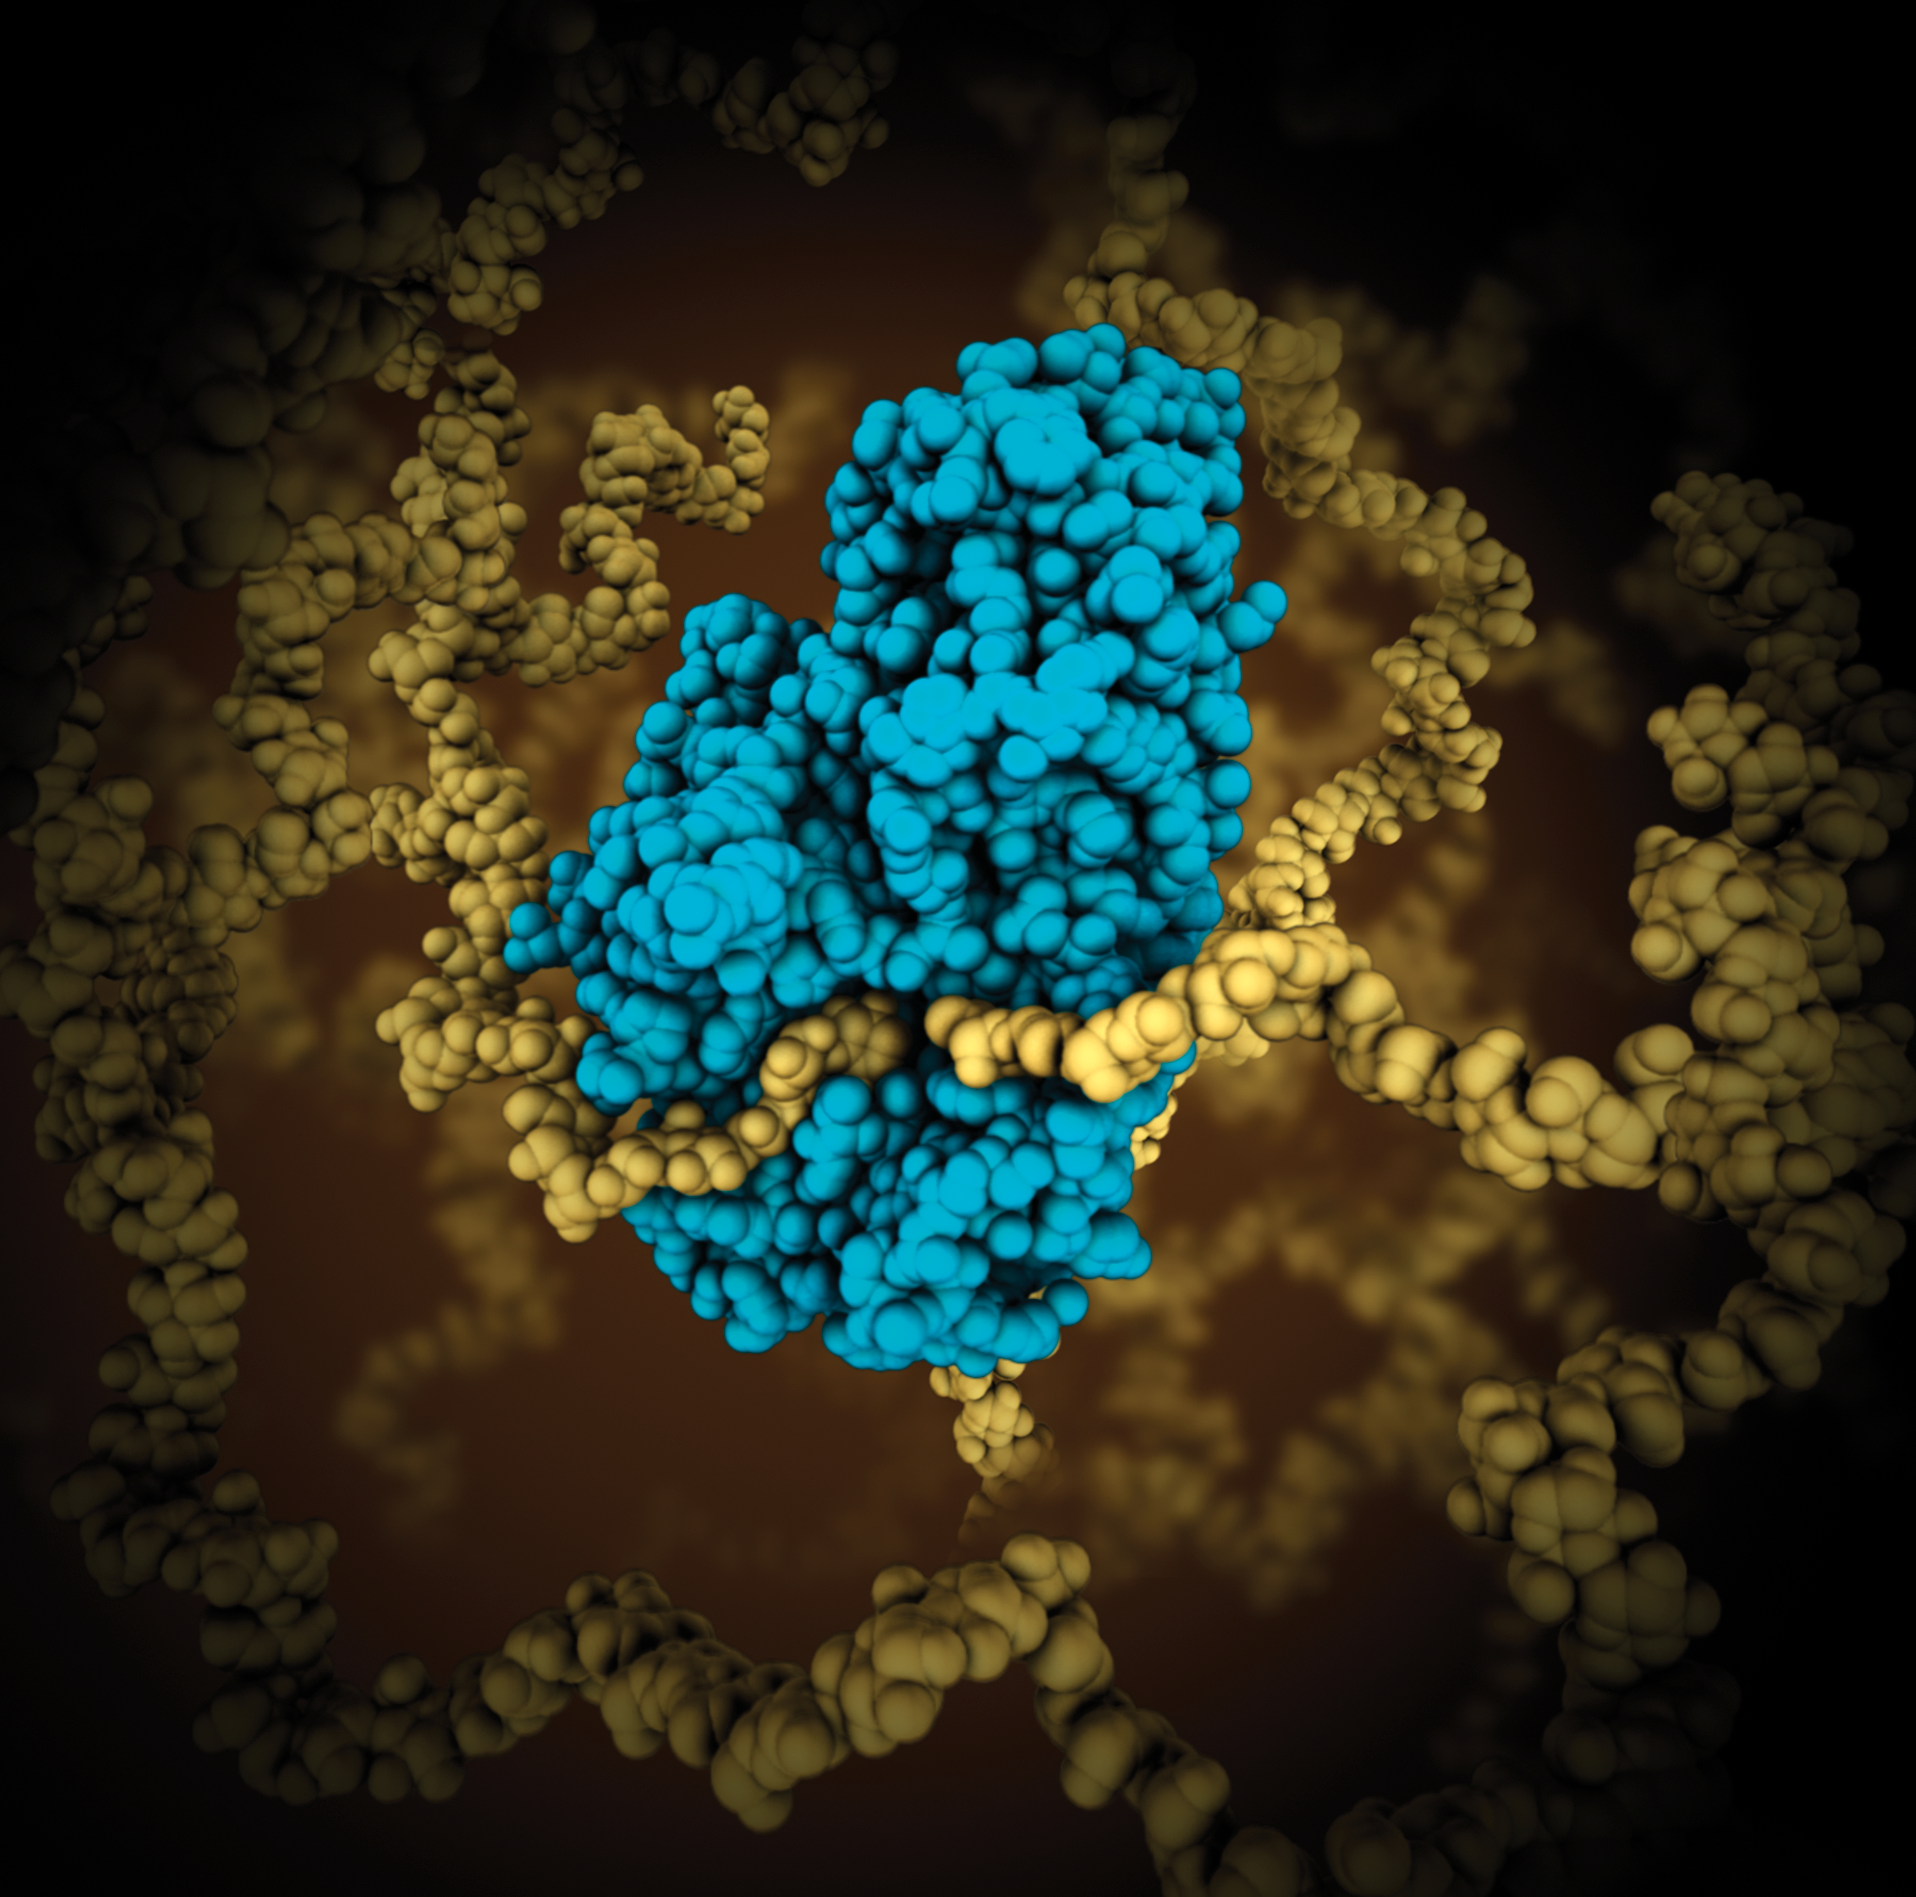
\includegraphics[scale=0.11]{images/Alpha-amylase.png}
	\caption{Enzima alpha Amilasi in turchese, rappresentazione di tipo space-filling. Si lega a catene di carboidrati (gialle) e le rompe in pezzi più piccoli di glucosio. Fonte \cite{ProteinRCSB}}
	\label{fig:amilasi}
	\endminipage\hfill
\end{figure}


Nelle cellule le proteine svolgono, fra le altre, funzioni di supporto strutturale, mobilità, protezione, regolazione, trasporto, catalisi, magazzino. Nel nostro corpo abbiamo un numero grandissimo di proteine: $10^{27}$. Per usare una metafora di Ken Dill \supercite{TalksDill2013Oct} potremmo dire che se si potesse ingrandire una proteina alla grandezza di un penny (diametro di 19mm) il numero di proteine che una persona ha nel corpo equivale al numero di penny che riempirebbero l'Oceano Pacifico.

\par Per queste e altre ragioni queste macromolecole sono il target di grandi attività di ricerca e di applicazione biotecnologiche: dal combattere malattie infettive \supercite{batool2019structure} al contrastare l'inquinamento ambientale \supercite{knott2020characterization}.

\section{Background informatico}

\subsection{Bioinformatica}

La \textit{bioinformatica} ha giocato un ruolo fondamentale durante l'epidemia di COVID-19, in particolare nella realizzazione di vaccini grazie agli avanzamenti nelle tecnologie NGS (Next Generation Sequencing). La bioinformatica è una disciplina dedicata alla risoluzione di problemi biologici a livello molecolare con metodi informatici, per questa ragione viene anche chiamata \textit{biologia computazionale}. Argomenti di interesse di questa disciplina sono:
\begin{itemize}
	\item allineamento di sequenze genetiche
	\item predizione genica
	\item predizione della struttura di proteine
	\item espressione genica
	\item interazione proteina-proteina
	\item interpretazione di dati proveniente da esperimenti biochimici
	\item organizzazione e archiviazione conoscenze su genomi e proteomi
	\item modellizzazione di sistemi e reti biologiche
\end{itemize}

\par Come si può notare da questa lista una parte importante della bioinformatica si occupa dell'utilizzo di strumenti informatici finalizzati a manipolare, archiviare e confrontare stringhe e sequenze di caratteri. Tuttavia questa disciplina non si ferma all’analisi delle sequenze. Tra le più interessanti applicazioni bioinformatiche odierne vi sono quelle incentrate sull’analisi strutturale \supercite{baxevanis2020bioinformatics}. Difatti la bioinformatica pone le sue fondamenta nel campo della \textit{structural bioinformatics}: per portare un esempio il database PDB (\textit{Protein Data Bank}) nasce nel 1977 per archiviare coordinate atomiche e legami derivati dagli studi cristallografici sulle proteine \supercite{bernstein77}.

\par Non va confusa la bioinformatica (o biologia computazionale) con la \textit{computazione bio-ispirata} (es. algoritmi genetici, reti neurali), con il \textit{biological computing} (ossia computer composti di parti biologiche come DNA, proteine o neuroni) o con la \textit{biological computation} (l'idea che gli organismi eseguano computazioni e che l'idea di informazione e computazione possa essere la chiave per comprendere la biologia)\supercite{Mitchell2010}.

\par Il Machine Learning (ML) è uno dei paradigmi informatici che più sta influenzando il campo della bioinformatica (come la presente tesi può dimostrare). Questo è dovuto principalmente a due fattori evolutisi in parallelo negli ultimi anni: la crescita esponenziale di dataset biologici disponibili e i progressi informatici del ML. Gli strumenti di ML possono apprendere caratteristiche dei sistemi biologici inferendole direttamente dai dataset. Quando propriamente allenati questi sistemi possono fornire accurate predizioni di caratteristiche astratte, proprio come nel caso di AlphaFold per il problema della predizione della struttra di proteine.

\subsection{Soft computing}
Il \textit{soft computing} è un paradigma che si contrappone a quello dell'\textit{hard computing}, ovvero la risoluzione di un problema tramite l'esecuzione di un algoritmo ben definito e decidibile. Il soft computing accantona la precisione od ottimalità e innalza a obiettivo il guadagno nella comprensione del comportamento di un sistema. Il soft computing si basa su due principi: 
\begin{enumerate}
	\item l'apprendimento a partire dai dati
	\item l'integrazione di conoscenza umana basata sull'esperienza, strutturata e preesistente, all'interno di modelli matematici computabili
\end{enumerate}

Il ML si avvale delle tecniche del soft computing \supercite{MLwiki} e vi entra pienamente: la stima di performance in ML è infatti l'\textit{accuratezza predittiva}, stimata dall'errore calcolato sul test set.

\begin{figure}[!h]
	\centering
	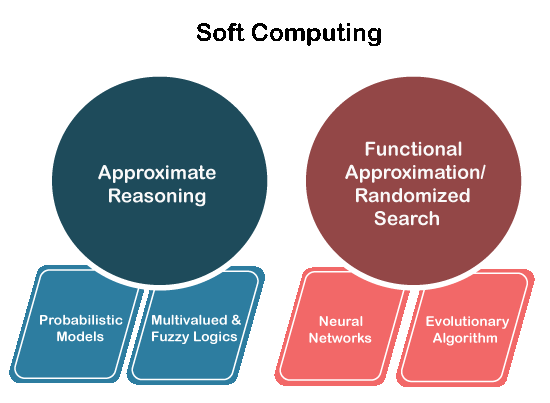
\includegraphics[scale=0.4]{images/soft-computing.png}
	\caption{Branche del soft computing. Fonte: \cite{softComputing}}
	\label{fig:soft-computing}
\end{figure}

\subsubsection{Algoritmi genetici}

\par Gli algoritmi genetici fanno parte del paradigma relativo alle tecniche informatiche \textit{bio-ispirate}, così come le reti neurali. Un algoritmo genetico è un algoritmo euristico utilizzato per tentare di risolvere problemi di ottimizzazione. L'aggettivo "genetico", ispirato al principio della selezione naturale ed evoluzione biologica, deriva dal fatto che, al pari del modello evolutivo darwiniano che trova spiegazioni nella genetica, gli algoritmi genetici attuano dei meccanismi concettualmente simili a quelli dei processi biochimici genetici, come il \textit{crossover}.

\subsection{Intelligenza Artificiale}

Definire cosa sia l'intelligenza non è un compito semplice. Una definizione ampia e utilizzata nel mondo dell'AI è quella data da Kurzweil:

\say{\textit{L’arte di creare macchine che svolgono funzioni che richiedono intelligenza quando svolte da esseri umani}}\footnote{\fullcite{kurzweil1990age}} \\

Una definizione di intelligenza proveniente da uno sfondo culturale del tutto diverso è la seguente:

\say{\textit{The role of intelligence is to determine the positive and negative potential of an event or factor which could have both positive and negative results. It is the role of intelligence, with the full awareness that is provided by education, to judge and accordingly utilize the potential for one's own benefit or well-being}}\footnote{\fullcite{dalaiLama}} \\

Nella sua accezione più semplice, l'Intelligenza Artificiale (AI) si riferisce a sistemi che imitano l'intelligenza umana per eseguire certe attività e che sono in grado di migliorarsi continuamente in base alle informazioni raccolte. L'IA si occupa della costruzione di macchine intelligenti, della comprensione mediante modelli computazionali dei comportamenti e della psicologia di uomini, animali e agenti artificiali e può avere applicazioni innumerevoli nella società. I fondamenti dell'IA sono sin dalla nascita interdisciplinari: filosofia, matematica, economia, neuroscienze, psicologia, informatica, linguistica, cibernetica, statistica, complessità, teoria del controllo, teoria dell'informazione, robotica.

\begin{figure}[!h]
	\centering
	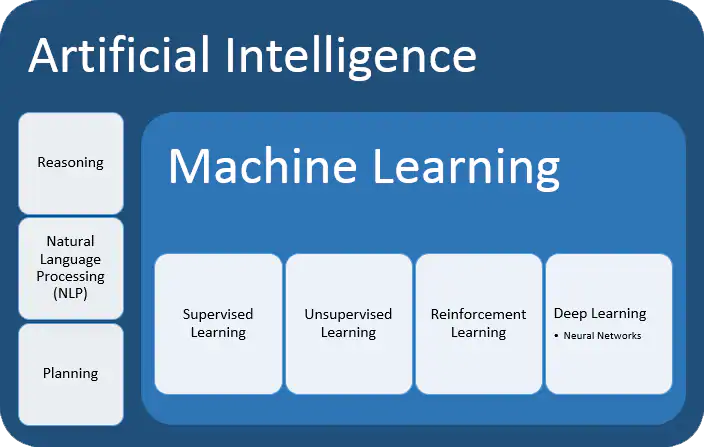
\includegraphics[scale=0.4]{images/artificial-intelligence.png}
	\caption{Schema riassuntivo dei campi dell'IA. Fonte: \cite{ML_IBM}}
	\label{fig:ai}
\end{figure}

\subsection{Machine Learning}

Il Machine Learning (ML) è un sottoinsieme dell'AI che si occupa di creare sistemi che automaticamente migliorano con l'esperienza, basandosi su rigorosi fondamenti delle scienze computazionali. Utilizza metodi statistici per migliorare la performance di un algoritmo nell'identificare pattern nei dati. Domande fondamentali di questo campo sono del tipo: "come varia la performance di apprendimento al variare del numero di esempi di allenamento presentati?". 

\par L'apprendimento è al cuore del problema dell'intelligenza sia bologica che artificiale ed è un principio universale comune a tutti gli organismi. Tom M. Mitchell definisce in questo modo l'apprendimento per una macchina:

\say{\textit{Si dice che un programma apprende dall'esperienza E con riferimento ad alcune classi di compiti T e con misurazione della performance P, se le sue performance nel compito T, come misurato da P, migliorano con l'esperienza E.}}\footnote{\fullcite{mitchell1997machine}} \\

Il ML si divide in:

\begin{itemize}
	\item \textit{Supervised Learning}, ad es. SVM (support vector machine), in cui al modello vengono forniti degli esempi nella forma di possibili input e i rispettivi output desiderati e l'obiettivo è quello di estrarre una regola generale che associ l'input all'output corretto; comuni sono i task di classificazione e regressione \\
	
	\item \textit{Unsupervised Learning}, in cui il modello ha lo scopo di trovare una struttura negli input forniti, come un raggruppamento naturale nei dati, senza che gli input vengano etichettati in alcun modo \\
	
	\item \textit{Reinforcement Learning}, il modello interagisce con un ambiente dinamico nel quale cerca di raggiungere un obiettivo (per esempio guidare un veicolo, o imparare a giocare contro un avversario), avendo un insegnante che gli dice solo se ha raggiunto l'obiettivo \\
	
	\item \textit{Deep Learning}, insieme di tecniche basate su reti neurali artificiali organizzate in diversi strati, dove ogni strato calcola i valori per quello successivo; si basa su diversi livelli di rappresentazione, corrispondenti a gerarchie di caratteristiche
\end{itemize}

Il ML è quindi sì uno strumento molto potente ma è importante comprenderne i limiti. È utile quando non esiste o è difficile da formalizzare la teoria attorno ad un problema, oppure quando i dati da analizzare sono incerti, rumorosi o incompleti.

\subsection{Reti neurali artificiali (ANN)}

Una rete neurale artificiale (\textit{Artificial Neural Network}) è un modello computazionale composto da neuroni artificiali bio-ispirato alla semplificazione di una rete neurale biologica. È importante notare che l'obiettivo della modellizzazione bio-ispirata non è una comprensione delle reti neurali biologiche, data la semplicità dei modelli utilizzati, ma il tentativo di risolvere problemi ingegneristici sfruttando idee derivanti da queste. Nonostante ciò le ANN riflettono tratti di comportamento del cervello umano e consentono di riconoscere pattern e risolvere problemi difficili.

\begin{figure}[!h]
	\centering
	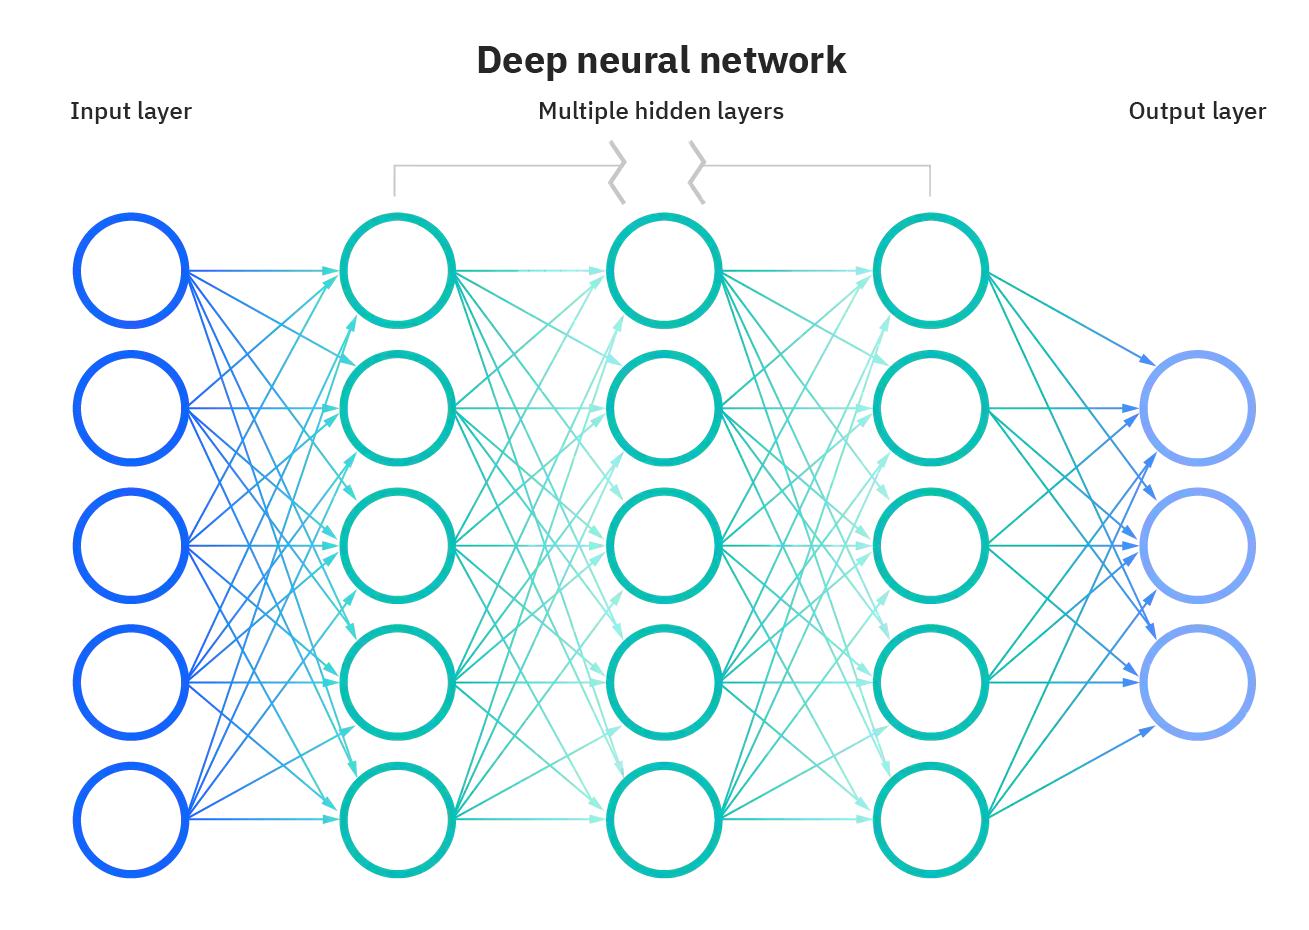
\includegraphics[scale=0.2]{images/ann.png}
	\caption{Rete neurale artificiale. Fonte: \cite{neuralNetworksIBM}}
	\label{fig:rete-neurale}
\end{figure}

\par Le ANN sono composte da strati di nodi: uno strato di input, uno o più nascosti e uno di output. Ogni nodo è un neurone artificiale, si connette a tutti i nodi dello strato successivo e ha associato un peso e una soglia. Se l'output di un nodo è sopra la soglia allora il neurone è attivato, trasferendo informazioni al prossimo strato della rete. Con l'allenamento le ANN possono migliorare la loro accuratezza e rivelarsi potenti strumenti. Campi di utilizzo sono, fra gli altri, lo \textit{speech-recognition} e l'{image recognition}.

\par La parola "deep" in \textit{deep learning} si riferisce alla profondità degli strati in una rete neurale. Una rete neurale artificiale che consiste in più di 3 strati (inclusi quello di input e output) può essere considerata un algoritmo di \textit{deep learning}\supercite{neuralNetworksIBM}. Una rete neurale con 2 o 3 strati è una rete neurale semplice.

\clearpage
%\chapter{Protein Folding}

\say{\textit{la forma è l'immagine plastica	della funzione}}\footnote{\fullcite{ruffini1925fisiogenia}}\\

La correlazione tra forma e funzione si rivela fondamentale nel caso delle proteine. Un canale ionico neuronale permette il passaggio di ioni grazie alla sua forma a canale; una ferritina cattura e immagazzina gli ioni ferro grazie alla sua forma a sfera cava. 

\par Il ripiegamento delle proteine (\textit{protein folding}) è il processo di ripiegamento molecolare attraverso il quale a partire dalla sequenza lineare amminoacidica le proteine ottengono la loro struttura tridimensionale, chiamata forma \textit{nativa}, che permette loro di svolgere la relativa funzione biologica. 

\begin{figure}[htp]
	\centering
	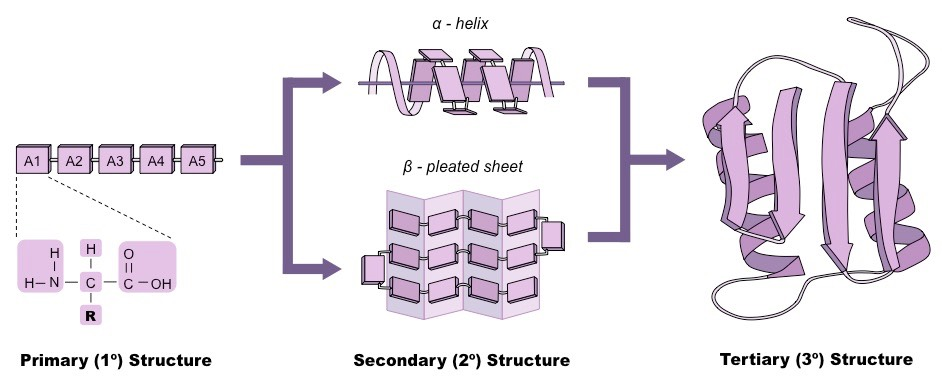
\includegraphics[scale=0.5]{images/protein-folding_med.jpeg}
	\caption{Protein folding: dagli amminoacidi alla struttura tridimensionale. Fonte: \cite{proteinStrucBioNinja}}
	\label{fig:protein-folding-bioninja}
\end{figure}


Il ripiegamento nella forma tridimensionale avviene spontaneamente sia durante la sintesi proteica nei ribosomi sia al termine di questa. Una specifica proteina si ripiegherà nello stesso modo e avrà la stessa struttura finale\footnote{ciò non è vero nel 100\% dei casi, alcune proteine possono avere più di una conformazione stabile per adempiere funzioni diverse (vedi la sezione \ref{sec:fold-switching-proteins}) e alcune proteine possono andare incontro a misfolding (vedi la sezione \ref{sec:assisted-folding})}.

\par La prima teoria del ripiegamento proteico è stata proposta negli anni venti del 20° secolo da Hsien Wu\supercite{wu1931studies}, in relazione al processo di denaturazione (vedi sezione \ref{sec:denaturazione}). È però Anfinsen, premio Nobel per la chimica, negli anni '60 a compiere un fondamentale passo nella comprensione del processo del ripiegamento proteico\supercite{anfinsen1972formation}. 


\section{Postulato di Anfinsen}
Il postulato di Anfinsen (conosciuto anche come \textit{dogma} o \textit{ipotesi termodinamica} di Anfinsen) afferma che la struttura nativa delle proteine (almeno quelle globulari) è determinata solamente dalla sequenza di amminoacidi di cui sono costituite. In altri termini: la struttura nativa, in ambiente fisiologico standard, corrisponde a quella struttura unica, stabile e cineticamente accessibile avente \textit{minima energia libera}. 

\begin{figure}[h]
	\centering
	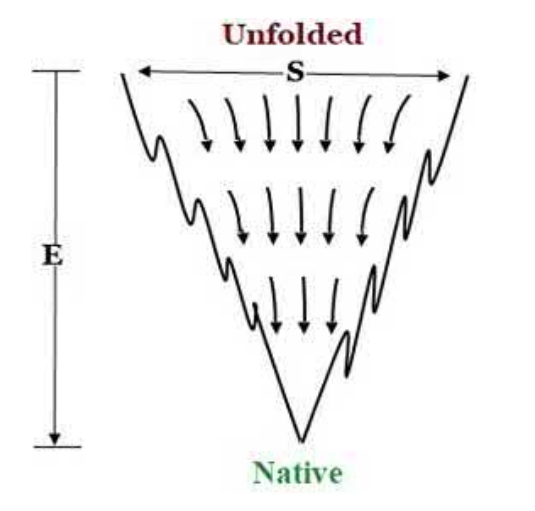
\includegraphics[scale=0.3]{images/funnel-folding.png}
	\caption{Un "panorama" idealizzato dell'energia libera a forma di imbuto. E=energia, S=entropia. Fonte: \cite{pal2019fundamentals}}
	\label{fig:funnel}
\end{figure}

Vi sono quindi 3 condizioni:

\begin{enumerate}
	\item \textit{unicità}, la sequenza non deve possedere altre configurazioni dotate di energia libera comparabile
	\item \textit{stabilità}, piccoli cambiamenti nell'ambiente circostante non possono produrre cambiamenti nella configurazione a energia minima. Ciò può essere descritto come una superficie parabolica di energia libera con lo stato nativo corrispondente al punto di minimo (visivamente simile ad un imbuto, vedi fig.\ref{fig:funnel}); la superficie di energia libera nelle vicinanze dello stato nativo deve essere abbastanza ripida ed elevata
	\item \textit{accessibilità cinetica}, il percorso nella superficie di energia libera dallo stato \textit{unfolded} a \textit{folded} deve essere ragionevolemente piano
\end{enumerate}


\subsection{Esperimento di Anfinsen}
L'esperimento, compiuto nel 1957\supercite{anfinsen1961kinetics}, consisteva nella denaturazione e rinaturazione della ribonucleasi A, dimostrando che il secondo processo era possibile senza agenti ausiliari. L'enzima in questione è formato da 124 amminoacidi, tra cui 8 cisteine che formano 4 ponti disolfuro ($-CH_{2}-\textbf{S-S}-CH_{2}-$). È stato usato un agente riducente per scindere questi ponti e l'urea per denaturare la proteina: questa non mostrava più alcuna attività enzimatica. A questo punto se l'urea era rimossa prima, seguita dall'aggiunta di un agente ossidante per consentire ai ponti disolfuro di riformarsi, la ribonucleasi A riacquistava spontaneamente la sua struttura terziaria e il prodotto ottenuto risultava praticamente indistinguibile dalla proteina nativa di partenza, riottenendo piena attività biologica. 

\begin{figure}[h]
	\centering
	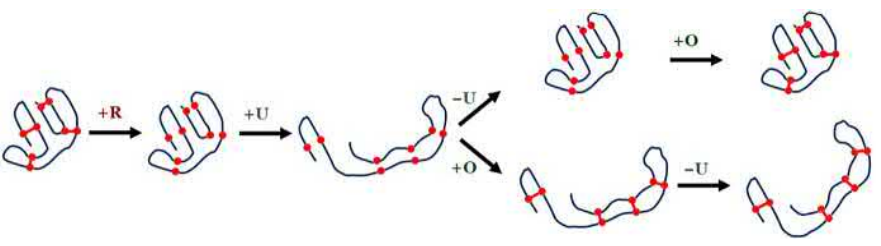
\includegraphics[scale=0.6]{images/anfinsen-experiment.png}
	\caption{Rappresentazione schematica dell'esperimento di Anfinsen. R=reducing agent, U=Urea, O=oxidizing agent, punti rossi=cisteina, linee rosse=ponti disolfuro. Fonte: \cite{pal2019fundamentals}}
	\label{fig:anfinsen-exp}
\end{figure}

I ponti disolfuro si riformano nella stessa posizione della proteina nativa nonostante ci siano 105 modi possibili per ricombinarli. Se invece veniva prima aggiunto l'agente ossidante e poi tolta l'urea il prodotto ottenuto era un miscuglio di molte delle possibili 105 configurazioni, raggiungendo solamente l'1\% dell'attività enzimatica.

\begin{figure}[!htb]
	\minipage{0.45\textwidth}
	\centering
	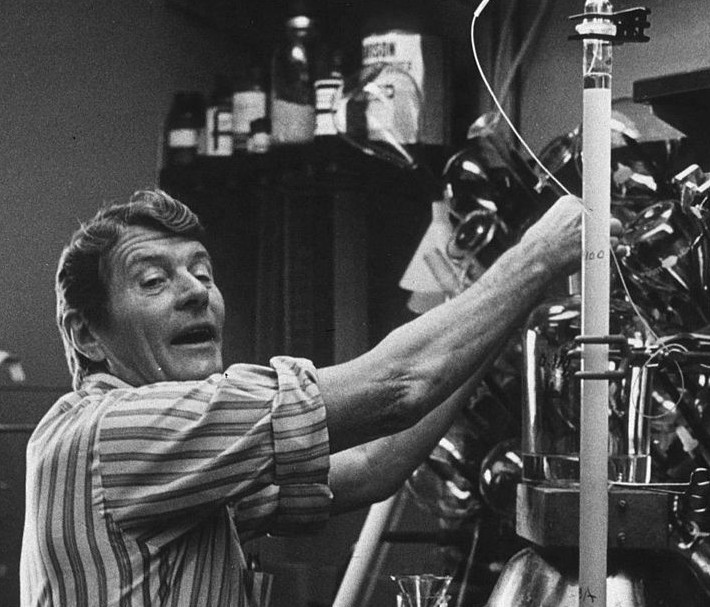
\includegraphics[scale=0.25]{images/anfinsen.jpg}
	\caption{C.B. Anfinsen nel suo laboratorio. Fonte: \cite{anfinsenNIH}}
	\label{fig:anfinsen}
	\endminipage\hfill
	\minipage{0.5\textwidth}
	\centering
	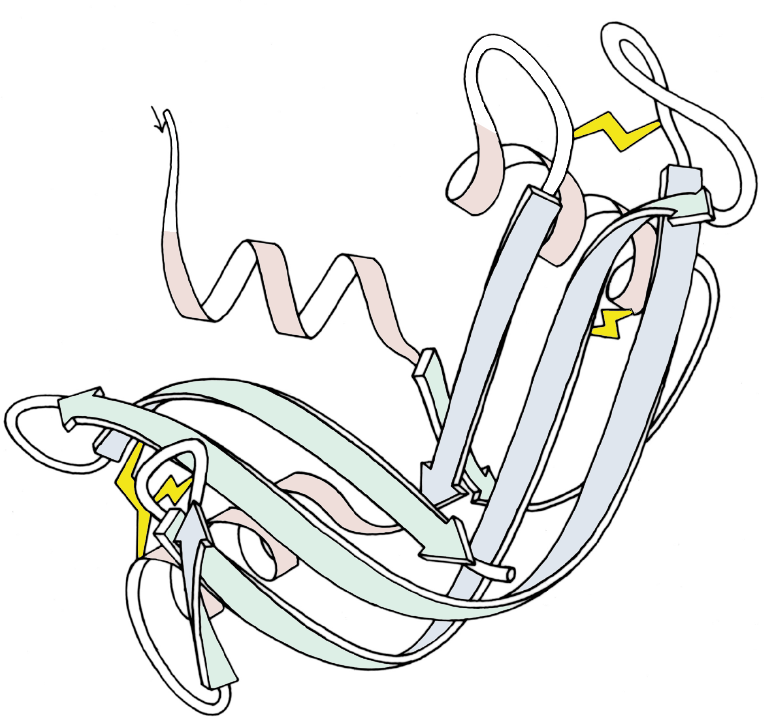
\includegraphics[scale=0.2]{images/RibonucleaseA_SS_paleRib.png}
	\caption{Ribonucleasi A, rappresentazione a nastro. In giallo i ponti disolfuro, rosa le $\alpha$-eliche, verde e azzurro i $\beta$-foglietti. Fonte \cite{ribonucleasi-file}}
	\label{fig:ribonucleasi}
	\endminipage\hfill
\end{figure}

\subsection{Denaturazione} \label{sec:denaturazione}
La denaturazione delle proteine è il fenomeno relativo all'alterazione della struttura nativa dovuto a variazioni di temperatura, pH o contatto con determinate sostanze chimiche. La denaturazione è un processo che porta alla perdita di ordine e quindi ad un aumento di entropia. La struttura primaria rimane invariata, data la stabilità dei legami peptidici. A causa della denaturazione le proteine perdono la loro funzione biologica e possono esporre e rendere reattivi alcuni gruppi funzionali che possono causare l'aggregazione di più proteine. Può avvenire che una volta rimosso l’agente denaturante la proteina ritorni allo stato di partenza (\textit{rinaturazione}) ma spesso il processo è irreversibile.

\begin{figure}[h]
	\centering
	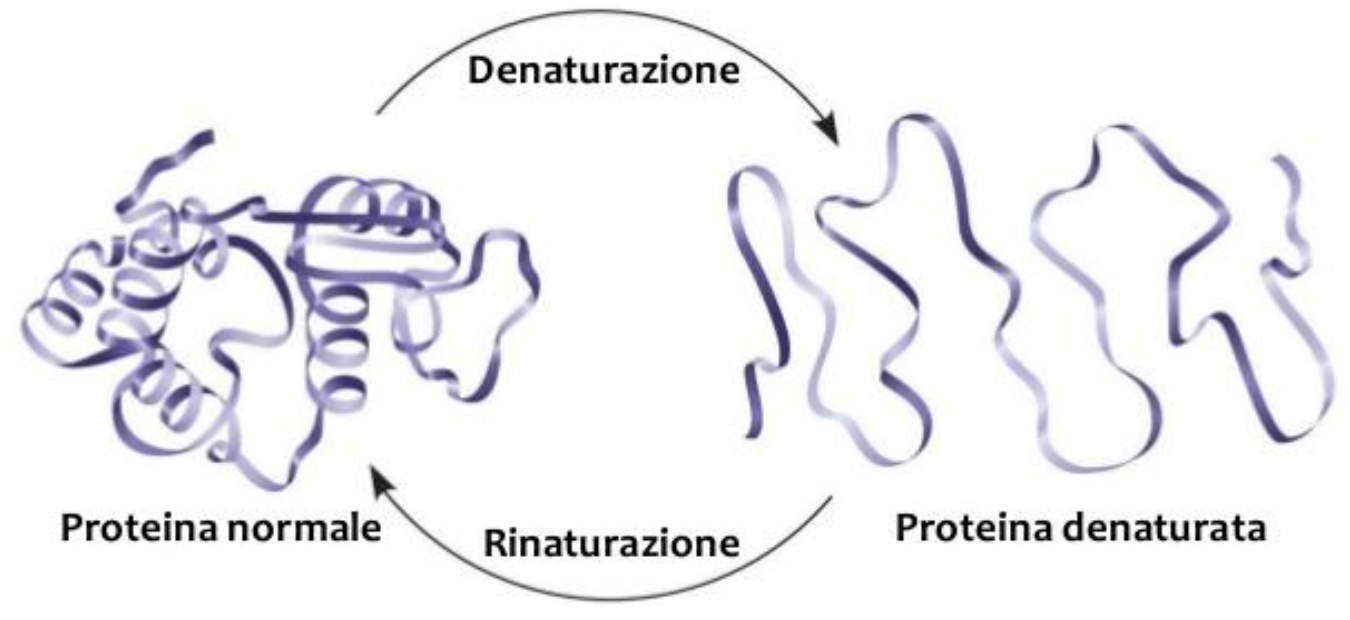
\includegraphics[scale=0.3]{images/denaturazione-rina.png}
	\caption{Denaturazione e rinaturazione. Fonte: \cite{campbell}}
	\label{fig:denaturazione}
\end{figure}

\par La proprietà di certe sostanze chimiche (es. urea) di denaturare una molecola proteica si deve alla loro capacità di legare transientemente, attraverso legami deboli, come ad esempio legami idrogeno, i residui amminoacidici costituenti la proteina. Questi legami vengono termodinamicamente preferiti a quelli intramolecolari o intermolecolari con l'acqua. Ciò comporta l'impossibilità per la proteina di mantenere la propria struttura tridimensionale e quindi questa si denatura. 

\par Applicazioni nella vita quotidiana di questo fenomeno sono la cottura dei cibi (basti pensare all'albumina nell'uovo) e la permanente ai capelli (denaturazione dell' $\alpha$-cheratina, rompendo e riformando ponti disolfuro). 


\section{Struttura delle proteine}
Da un punto di vista chimico le proteine sono di gran lunga, tra quelle conosciute, le molecole strutturalmente più complesse e sofisticate funzionalmente. È possibile studiare la loro struttura individuando successivi livelli di organizzazione:

\begin{figure}[!htp]
	\centering
	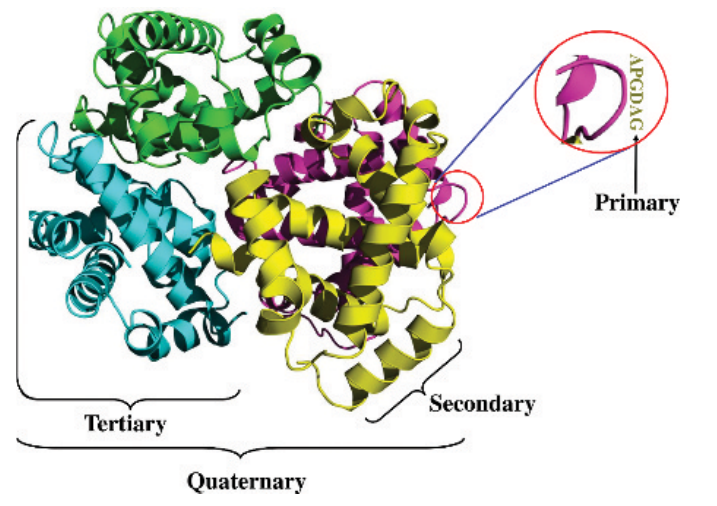
\includegraphics[scale=0.4]{images/strutture-proteina.png}
	\caption{Giri e Loop. Fonte: \cite{kessel_ben-tal_2018}}
	\label{fig:strutture-proteine}
\end{figure}

\begin{itemize}
	\item \textit{struttura primaria}: la sequenza ordinata degli amminoacidi
	\item \textit{struttura secondaria}: regioni ripetitive locali stabilizzate da legami idrogeno tra atomi della backbone ($\alpha$-eliche e $\beta$-foglietti)
	\item \textit{struttura supersecondaria}: combinazione di strutture secondarie e connessioni (motivi, domini, loop, giri ...)
	\item \textit{struttura terziaria}: forma tridimensionale di una singola catena polipeptidica, risultante dalle interazioni dei residui
	\item \textit{struttura quaternaria}: forma finale di proteine "assemblate" da 2 o più catene polipeptidiche già ripiegate
\end{itemize}

Prima di passare ad analizzare ogni livello della struttura delle proteine è utile un veloce sguardo alle interazioni molecolari.

\subsection{Interazioni molecolari}

\begin{itemize}
	\item \textit{legame covalente}: prevede la compartecipazione di 2 elettroni di valenza fra più atomi ed è il tipo di legame più forte (kcal/mol). Due o più atomi tenuti insieme da legami covalenti formano una molecola
		\begin{itemize}
			\item \textit{elettronegatività}:
		\end{itemize}
		
	\item \textit{legami non covalenti}
		\begin{itemize}
			\item \textit{legame ionico}: l'atomo più elettronegativo strappa completamente un elettrone al suo compagno, si formano due ioni (uno positivo, \textit{catione} e uno negativo, \textit{anione})
			\item \textit{legame idrogeno}: un atomo di idrogeno si trova fra due atomi elettronegativi vicini; ad es. nell'acqua gli atomi di idrogeno (parzialmente positivi) si trovano fra due atomi di ossigeno (parzialmente negativi). L'idrogeno, legato a uno dei due atomi di ossigeno, permette all'altro di avvicinarsi e di stabilizzarsi
			\item \textit{interazioni di van der Waals}: nelle molecole apolari gli elettroni si possono accumulare in modo asimmetrico, formando regioni momentaneamente polari che permettono così una temporanea stabilizzazione fra molecole a breve distanza
		\end{itemize}
	\item \textit{effetto idrofobico}: 
	\item 
\end{itemize}
\begin{itemize}
	\item \textit{ponte disolfuro}, lo zolfo di una cisteina si lega allo zolfo della seconda cisteina.
\end{itemize}

• una forza dominante o tante piccole forze?\\
• Cambio di paradigma da metà anni ‘80\\

\subsubsection{Struttura primaria}
La struttura primaria delle proteine è la sequenza ordinata degli amminoacidi che ne determina la conformazione nativa. La posizione nella sequenza di specifici amminoacidi è un fattore fondamentale per la determinazione di quali porzioni della proteina andranno a legarsi formando globalmente la struttura finale. La nota importante, basata sul dogma di Anfinsen, è che la sequenza amminoacidica di ogni proteina contiene l'informazione che specifica sia la struttura nativa che la via per raggiungere quello stato. Questo comunque non vuol dire che strutture simili si ripieghino in modo simile.
	
\subsubsection{Struttura secondaria}

La struttura secondaria riguarda le regioni ripetitive locali stabilizzate da legami idrogeno tra atomi della backbone: ($\alpha$-eliche e $\beta$-foglietti).

\begin{figure}[h]
	\centering
	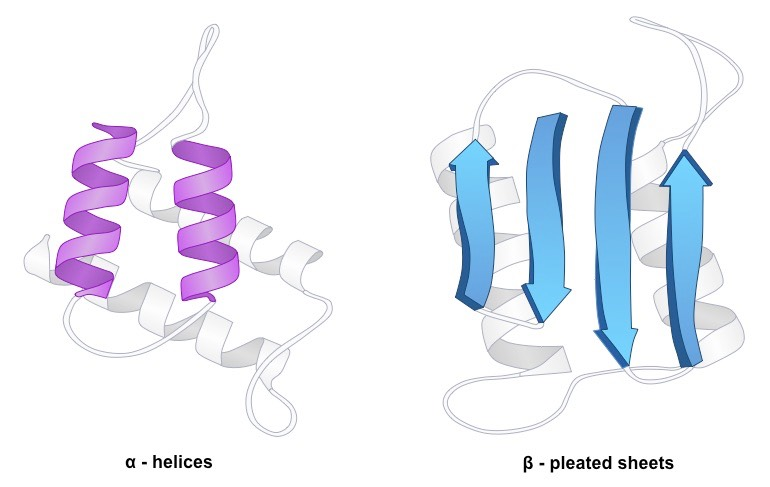
\includegraphics[scale=0.4]{images/secondary.jpeg}
	\caption{Struttura secondaria delle proteine, $\alpha$-eliche e $\beta$-foglietti. Fonte: \cite{proteinStrucBioNinja}}
	\label{fig:struttura-secondaria}
\end{figure}

Questo livello di organizzazione è una conseguenza dei legami a idrogeno tra gli amminoacidi appartenenti a una stessa catena, o tra gli amminoacidi di catene diverse.  All'interno della backbone del polipeptide gli atomi di ossigeno hanno una parziale carica negativa e gli atomi di idrogeno attaccati all'azoto hanno una parziale carica positiva perciò possono formarsi legami idrogeno fra questi atomi. Individualmente sarebbero deboli legami ma poiché sono ripetuti molte volte su di una regione relativamente lunga di una catena polipeptidica possono fare da supporto per una particolare conformazione.

\par Nella struttura ad $\alpha$-elica gli amminoacidi sono avvolti in una spirale tenuta insieme da legami idrogeno ogni 4 amminoacidi. Tra l’atomo di idrogeno legato all’azoto di ogni legame peptidico e l’ossigeno del gruppo carbossilico del legame peptidico sovrastante (che si trova appunto a distanza di quattro amminoacidi lungo la catena) si instaura un legame a idrogeno. Tuttavia se gli amminoacidi che si succedono lungo un tratto di catena proteica hanno gruppi R voluminosi, come avviene nella prolina, o gruppi R dotati della stessa carica elettrica, come avviene negli amminoacidi lisina e arginina, l’$\alpha$-elica non può formarsi, a causa delle forze di repulsione che si generano tra i residui. Alcune proteine fibrose, come l'$\alpha$-cheratina, la proteina strutturale dei capelli, la lana e le unghie hanno formazioni di $\alpha$-eliche sulla maggior parte della loro lunghezza.


\begin{figure}[!htp]
	\centering
	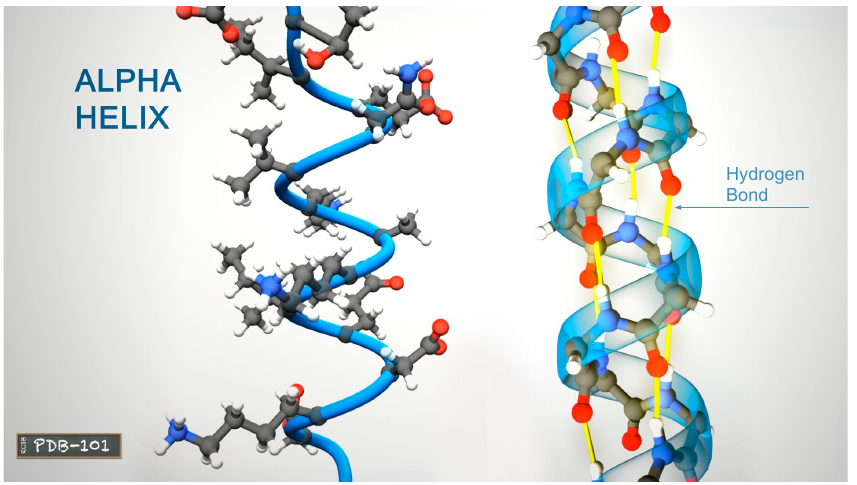
\includegraphics[scale=0.4]{images/alpha-helix.png}
	\caption{elica. Fonte: \cite{ProteinRCSB}}
	\label{fig:alpha-helix}
\end{figure}


\begin{figure}[!htp]
	\centering
	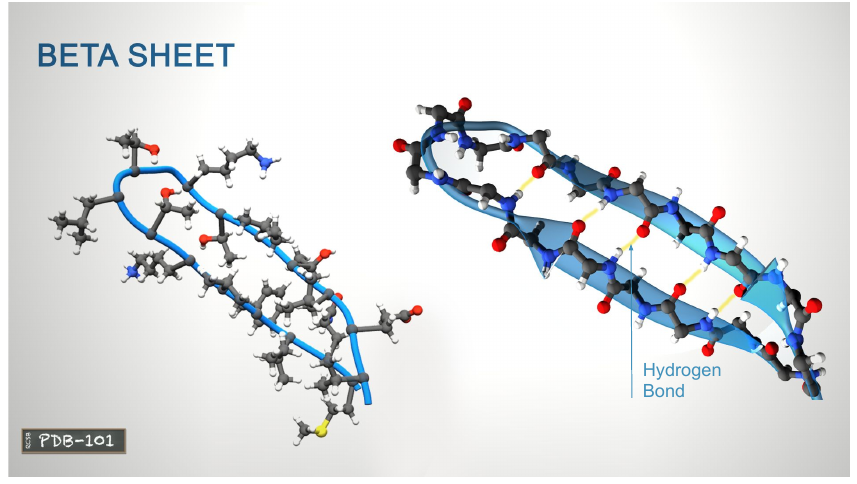
\includegraphics[scale=0.4]{images/beta-sheet.png}
	\caption{foglietto. Fonte: \cite{ProteinRCSB}}
	\label{fig:beta-sheet}
\end{figure}

\begin{figure}[!htb]
	\minipage{0.5\textwidth}
	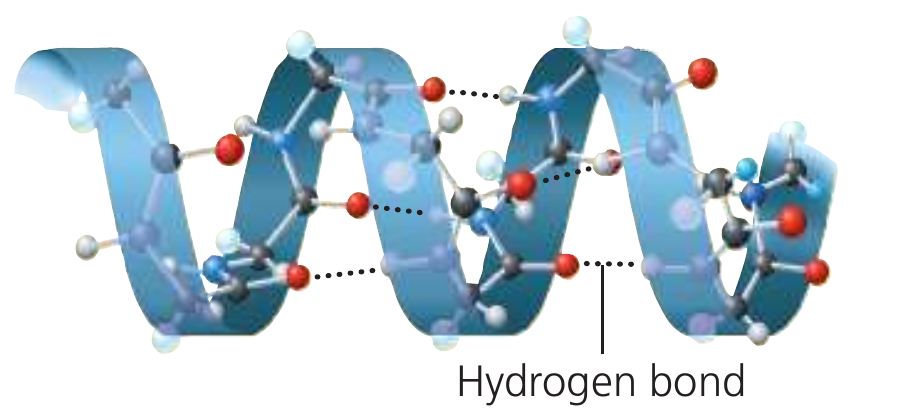
\includegraphics[scale=0.34]{images/eliche.png}
	\caption{Regione di $\alpha$-elica. Fonte: \cite{campbell}}
	\label{fig:eliche}
	\endminipage\hfill
	\minipage{0.5\textwidth}
	\centering
	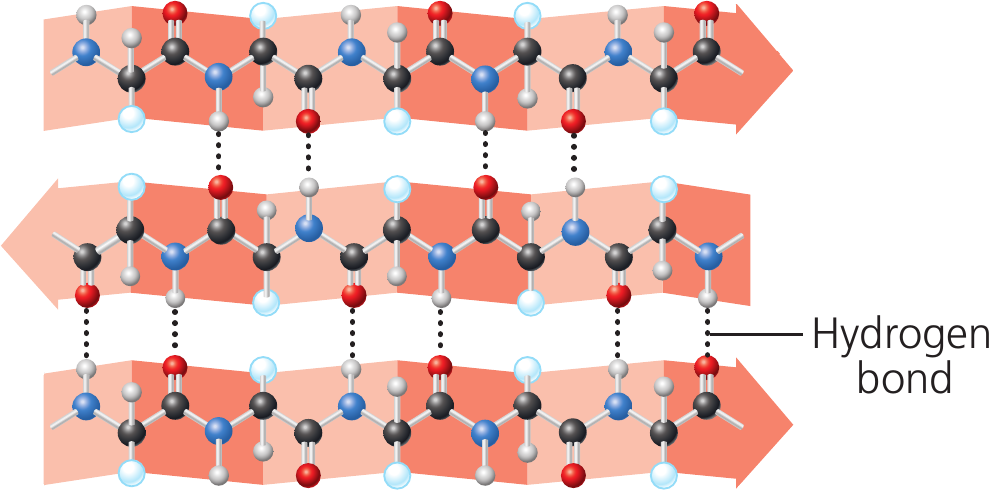
\includegraphics[scale=0.31]{images/foglietti.png}
	\caption{Una regione di $\beta$-foglietto composto da $\beta$-filamenti adiacenti, spesso mostrati come una freccia pieghettata o piatta puntata in direzione C-terminus. Fonte \cite{campbell}}
	\label{fig:foglietti}
	\endminipage\hfill
\end{figure}

Altre proteine fibrose sono invece dominate dai $\beta$-foglietti, come le proteine della seta ($\beta$-cheratina) e la tela prodotta dai ragni. In queste conformazioni due o più segmenti della catena polipeptidica giacenti lato su lato (chiamati $\beta$-filamenti) sono connessi da tre o più legami idrogeno. Si definisce $\beta$-filamento una sequenza peptidica di amminoacidi (tipicamente 5-10) che si dispone linearmente ed è in grado di formare legami idrogeno. Ciascuna delle catene è totalmente estesa e presenta una conformazione a zig-zag, dovuta alla geometria dei legami attorno a ciascun atomo di carbonio e di azoto nella catena. In questo caso, i legami a idrogeno si formano tra gli amminoacidi di due catene adiacenti. I gruppi amminici di uno scheletro peptidico formano legame con quelli carbossilici del filamento opposto. In ogni singolo filamento i residui si dispongono perpendicolarmente al piano del foglietto, puntando alternativamente verso l'alto e verso il basso.

\par Nella vita quotidiana, se tiriamo per i due estremi una fibra di lana questa si allunga: si stanno rompendo i legami idrogeno e le eliche si allontanano sempre di più, ma lasciando la presa i legami idrogeno si riformano e le eliche ricompaiono nella struttura. Se invece tiriamo la seta si può osservare che non è elastica: i foglietti di cui è composta la sua struttura non sono smantellabili senza rompere anche i legami covalenti della backbone.


\subsubsection{Struttura supersecondaria: Motivi, Domini, Loop, Giri ...}
La struttura supersecondaria è riferita alle combinazioni spaziali di strutture secondarie in conformazioni più complesse e alle connessioni che li uniscono. Può essere considerata come esempio di struttura supersecondaria la triplice elica allungata del collagene.

\par I \textit{motivi} (motifs) e \textit{domini} (domains) sono regioni tridimensionali della catena polipeptidica formate da differenti strutture secondarie adibite a svolgere una determinata funzione per la proteina di cui fanno parte. Tuttavia sono differenti in quanto i motivi non mantengono la loro forma se separati dalla proteina laddove i domini la mantengono. Questo perché i motivi e il resto della proteina sono più vicini e si vengono così a formare legami idrogeno che permettono ai motivi di mantenere la struttura. I domini sono sì legati alla backbone della proteina ma non abbastanza vicini alla restante parte della formazione proteica da stabilire legami, pertanto se vengono separati non perdono la loro struttura e possono mantenere la loro funzione.

\par Più in generale un \textit{motivo strutturale} è una struttura tridimensionale comune che appare in una varietà di molecole differenti ed evoluzionisticamente scollegate.

\begin{figure}[!htp]
	\centering
	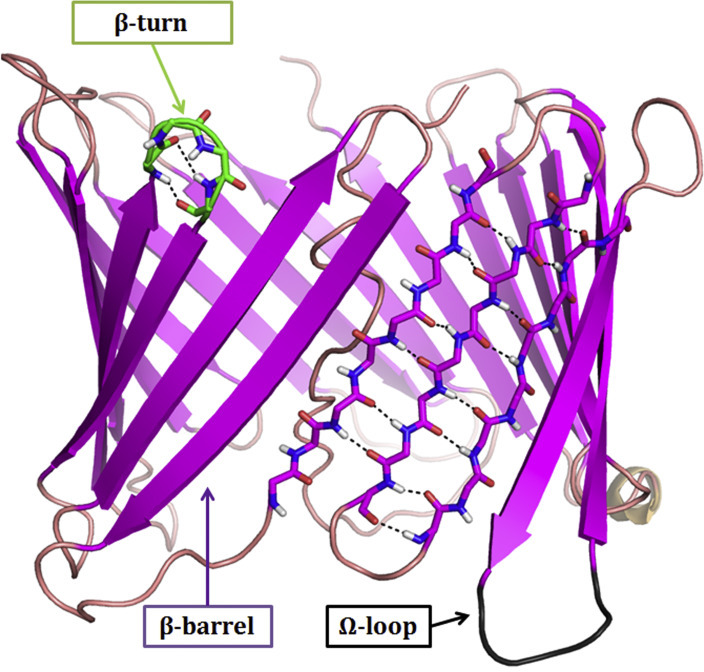
\includegraphics[scale=1.1]{images/turn-loop.jpg}
	\caption{Giri e Loop. Fonte: \cite{MURRAY2017477}}
	\label{fig:turn-loops}
\end{figure}


\par \textit{Giri} e \textit{loop} causano cambi di direzione alla backbone della proteina
Protein loops are patternless regions which connect two regular secondary structures. They are generally located on the protein's surface in solvent exposed areas and often play important roles, such as interacting with other biological objects. Despite the lack of patterns, loops are not completely random structures

\par Nelle strutture secondarie e terziarie si trovano spesso bruschi cambiamenti di direzione nella struttura: i \textit{giri} (turns). Queste nette svolte sono possibili grazie agli amminoacidi prolina e glicina. Il gruppo R della prolina si ripiega verso il gruppo amminico, distorcendo la catena naturalmente. Si forma però uno stretto spazio a causa del giro: l'amminoacido con gruppo R meno voluminoso è ovviamente la glicina ed è per questo che si trovano insieme nei giri.

\subsubsection{Struttura terziaria}
La struttura terziaria è la struttura tridimensionale globale risultante dalle interazioni tra i residui successivamente alle conformazioni locali della struttura secondaria ed è quindi la descrizione del risultato del processo di ripiegamento proteico. Un tipo di interazione importante è quella idrofobica che induce i residui non polari (e quindi idrofobici) a raggrupparsi al centro della catena polipeptidica, formando un nucleo idrofobico. La forma della proteina può venire rinforzata dai ponti disolfuro, legami covalenti fra due cisteine.

\begin{figure}[!htp]
	\centering
	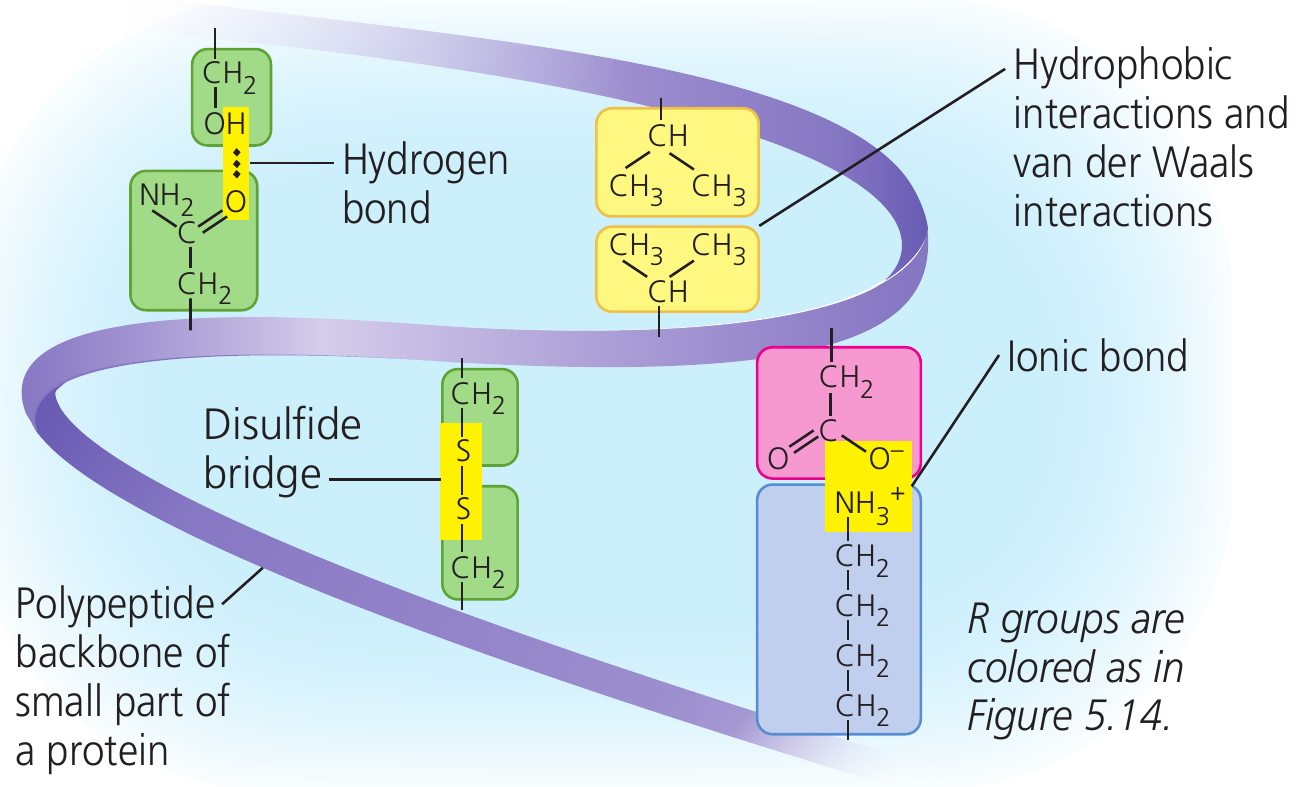
\includegraphics[scale=0.35]{images/interazioni-proteine.png}
	\caption{I diversi tipi di interazioni che possono contribuire alla struttura terziaria di una proteina. Fonte: \cite{campbell}}
	\label{fig:interazioni-proteine}
\end{figure}

\subsubsection{Struttura quaternaria}
La struttura quaternaria è la forma finale di proteine "assemblate" da 2 o più catene polipeptidiche già ripiegate. Il collagene ne è un esempio poiché è formata da 3 polipeptidi quasi interamente a spirale che si attorcigliano l'uno sull'altro formando un'elica tripla ancora più larga, dando alle lunghe fibre una grande forza. Un altro esempio è l'emoglobina, proteina globulare formata da 4 subunità polipeptidiche. Le strutture terziarie delle subunità non vengono alterate.

\begin{figure}[!htb]
	\centering
	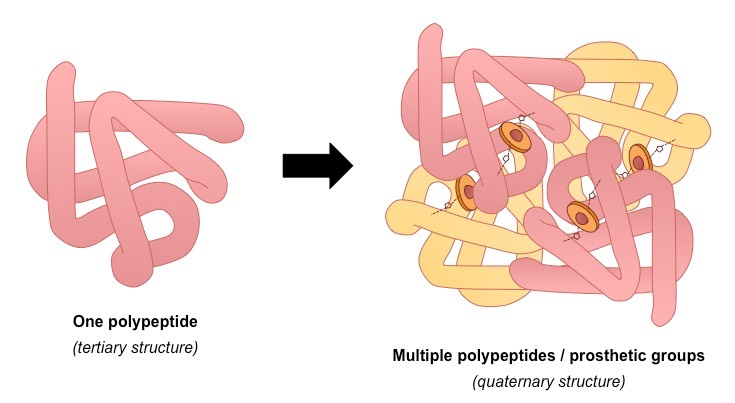
\includegraphics[scale=0.35]{images/quaternary-structure_med.jpeg}
	\caption{Rappresentazione di una struttura quaternaria composta da più polipeptidi e alcuni gruppi prostetica. Fonte \cite{proteinStrucBioNinja}}
	\label{fig:struttura-quaternaria}
\end{figure}

\subsection{Geometria dei legami?}

• Domini, Residui, Motivi, Giri, Loops, Turns\\

\section{Ripiegamento assistito} \label{sec:assisted-folding}
All'interno delle cellule le proteine più piccole si ripiegano indipendentemente, mentre proteine più grandi sono assistite principalmente da complessi chiamati \textit{chaperoni molecolari}. È  importante notare che l'assistenza è cinetica in natura: non aggiunge nuove informazioni necessarie alla proteina per ripiegarsi, pertanto il dogma di Anfinsen non viene contraddetto. Ciò che fanno questi complessi è creare un ambiente nel quale le proteine possano ripiegarsi senza "distrazioni" dovute a interazioni con altre entità (ad esempio evitando l'aggregazione con altre proteine) e senza rimanere bloccate in conformazioni intermedie durante il loro percorso di ripiegamento. In poche parole sono misure di protezione della cellula. 

\begin{figure}[h]
	\centering
	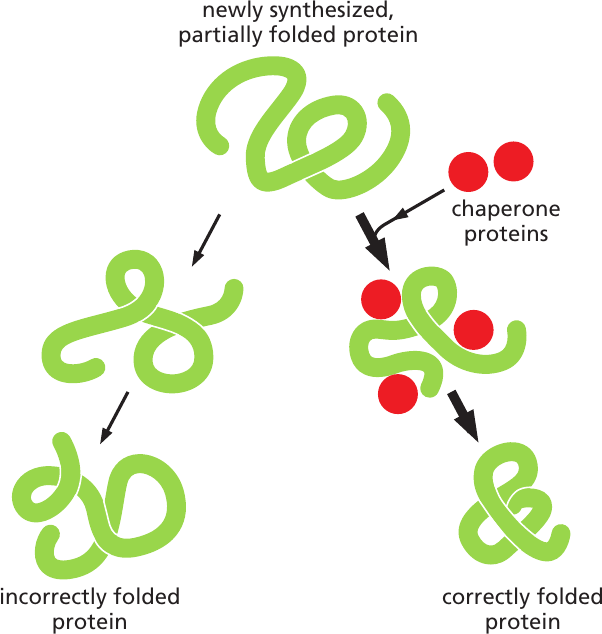
\includegraphics[scale=0.4]{images/chaperone-alberts.png}
	\caption{Schema della funzione dei chaperoni molecolari. Fonte: \cite{alberts2018essential}}
	\label{fig:chaperoni}
\end{figure}

Più in dettaglio i chaperoni molecolari svolgono le seguenti funzioni:
\begin{enumerate}
	\item assistono il corretto ripiegamento delle catene polipeptidiche (lunghe) appena sintetizzate
	\item dirigono l'assemblaggio di complessi multienzimatici
	\item donano una "seconda chance" a proteine danneggiate favorendone la rinaturazione
	\item partecipano nella parziale denaturazione durante il trasporto di proteine attraverso membrane di mitocondri o cloroplasti
\end{enumerate}

Tutti i compartimenti cellulari delle cellule eucariotiche (nucleo, citosol, reticolo endoplasmatico, mitocondri e cloroplasti) hanno il proprio set di chaperoni che assicura un corretto ripiegamento delle proteine. I chaperoni molecolari comprendono diverse famiglie di proteine altamente conservate, tra cui le Hsp (Heat shock protein), proteine espresse in grande quantità sotto condizioni di alto stress, per contrastarne l'effetto denaturante. Queste ultime sono state classificate in base al loro peso molecolare, ad es. Hsp60 dove "60" indica 60kDa. Le Hsp60 vengono chiamate anche \textit{chaperonine} e sono una famiglia di chaperoni molecolari a doppio anello che agiscono da "camera di isolamento" per il ripiegamento di altre proteine\supercite{ranson1998chaperonins}, famosa è la chaperonina procariotica GroEL (vedi fig.\ref{fig:groel}), che può essere assunta come modello di riferimento delle chaperonine. 

\begin{figure}[h]
	
\end{figure}

\begin{figure}[!htb]
	\minipage{0.35\textwidth}
	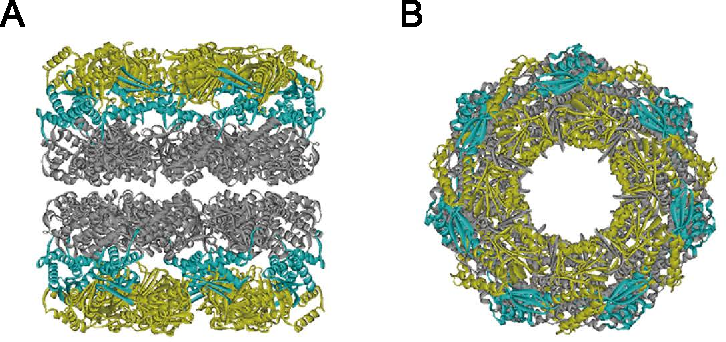
\includegraphics[scale=0.25]{images/groel.png}
	\caption{Strutture dei complessi GroEL e GroEL-GroES. (B) si può osservare la tipica forma ad anello. Fonte: \cite{Iizuka2016ChaperoninGU}}
	\label{fig:groel}
	\endminipage\hfill
	\minipage{0.6\textwidth}
	\centering
	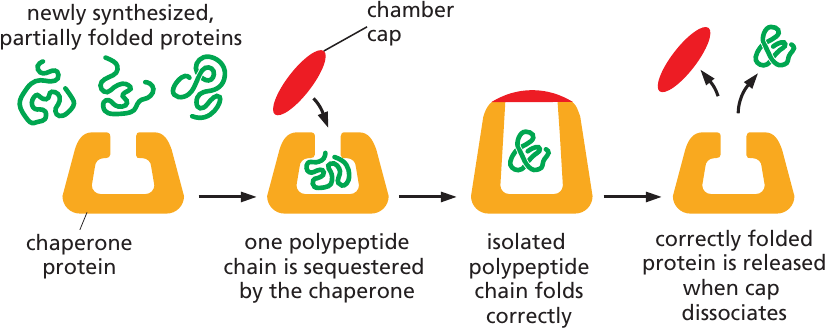
\includegraphics[scale=0.4]{images/chaperone-alberts-isolation.png}
	\caption{Rappresentazione schematica della funzione della camera di isolamento nelle chaperonine. Fonte \cite{alberts2018essential}}
	\label{fig:chaperone-camera}
	\endminipage\hfill
\end{figure}

Sebbene i mitocondri (e i cloroplasti) abbiano il loro genoma e creino le loro proteine, la maggior parte delle proteine che questi organelli usano sono codificate dai geni nel nucleo e importati dal citosol. Ogni proteina viene quindi parzialmente denaturata per effettuare il trasporto. I chaperoni molecolari all'interno di questi organelli aiutano a tirare le proteine attraverso le due membrane e a ripiegarle una volta all'interno\supercite{alberts2018essential}.


\subsection{Misfolding e malattie}

Il \textit{misfolding} è il fenomeno dell'errato ripiegamento di una proteina, ovvero quando una proteina non può raggiungere il suo stato nativo. Ciò può accadere per mutazioni alla sua sequenza amminoacidica, anche per un solo amminoacido differente (come nel caso dell'anemia falciforme) o per fattori esterni. Le proteine mal ripiegate tipicamente contengono $\beta$-foglietti organizzati in una struttura denominata cross-$\beta$, disposizione molto stabile e insolubile, generalmente resistente alla proteolisi. Il mal ripiegamento di alcune proteine può innescare ulteriori mal ripiegamenti e la conseguente accumulazione di proteine mal ripiegate in aggregati (od oligomeri) che possono guadagnare tossicità attraverso le interazioni intermolecolari. L'incremento dei livelli di proteine aggregate può portare alla formazione di \textit{amiloidi}, strutture fibrillari formate da deposizioni di materiale proteico insolubile. L'errato ripiegamento delle proteine è alla base quindi di molte patologie umane, definite malattie da misfolding, categorizzabili in due gruppi:

\begin{itemize}
	\item malattia causata dalla perdita o degradazione della proteina o dall'errato trasporto intracellulare
	\item malattie causate dall'accumulo, intra od extra-cellulare, di proteine aggregate (ad esempio le malattie da prione)
\end{itemize}

Molti tipi di tumore diventano chemio-resistenti perché iper-esprimono alcune Hsp, come la Hsp70 e la Hsp90. Le Hsp sono presenti anche in quantità elevatissime nel cervello dei pazienti con malattia di Alzheimer e morbo di Parkinson. Tuttavia si crede che la loro aumentata espressione non sia lesiva di per sé ma rappresenti piuttosto una risposta difensiva agli elevati livelli di stress che caratterizzano queste patologie. Ci sono molti morbi associati a mutazioni nei geni codificanti i chaperoni. Alterazioni genetiche delle chaperonine possono portare a patologie umane che in genere colpiscono molti organi ed apparati contemporaneamente \supercite{chaperoninaWiki}. \\

\par I \textit{prioni} (acronimo di "\textbf{pr}oteinaceous \textbf{i}nfective \textbf{on}ly particle") sono molecole di natura proteica con la capacità di trasmettere la propria forma mal ripiegata a varianti normali della stessa proteina. \footnote{I prioni sono stati studiati e denominati in questo modo dal premio Nobel per la medicina nel 1997 Stanley Prusiner\supercite{prusiner1998prion}} Il ruolo ipotizzato di una proteina come agente infettivo è in contrasto con tutti gli altri agenti infettivi conosciuti, come i viroidi, virus, batteri, funghi, parassiti: tutti contengono acidi nucleici (DNA, RNA o entrambi) mentre le proteine sono composte di soli amminoacidi.

\par I prioni formano amiloidi che si accumulano nei tessuti e sono associati a danni di questi e alla morte cellulare. I prioni sono attualmente considerati i più probabili agenti delle encefalopatie spongiformi trasmissibili (TSE) dei mammiferi. Nel \textit{morbo della mucca pazza} (encefalopatia spongiforme bovina), malattia neurologica degenerativa e irreversibile, vi è il ruolo di un prione a causare mal ripiegamenti di alcune proteine native causando la formazione di strutture amiloidi fatali (al microscopio le dense placche fibrose appaiono come buchi, da qui il caratteristico aspetto "a spugna"). Tutte le malattie da prione sono attualmente inguaribili e letali, con un periodo di incubazione che dura generalmente vari anni.

\par Gli aggregati di prioni sono stabili e questa stabilità strutturale consente loro di essere immuni alla maggior parte dei trattamenti conosciuti. L'organismo infettato non ha modo di degradarli: a differenza di virus e batteri i prioni rimangono intatti anche in presenza di trattamenti come sterilizzazione, forti dosi di radiazioni ionizzanti, uso di formaldeide, varechina, acqua bollente e a differenza delle altre proteine sono resistenti alla maggior parte delle proteasi.

\par La proteina di cui sono fatti i prioni, \textit{PrP} (protease-resistant-protein, Pr per \textbf{pr}ione, e P per \textbf{p}roteina), si trova in tutto il corpo, anche negli individui sani, ed è altamente conservata nei mammiferi. Tuttavia, la PrP trovata nel materiale infettante ha una struttura diversa. Nell'uomo la PrP$^{c}$(\textbf{c}ellulare, forma normale) è codificata da un solo gene, PRNP. La PrP$^{sc}$(\textbf{sc}rapie, forma patologica) differisce dalla proteina naturale PrP$^{c}$ per la conformazione tridimensionale: la PrP$^{c}$ ha una struttura più aperta contenente 3 segmenti ad $\alpha$-eliche e pochi $\beta$-foglietti; la PrP$^{sc}$ invece ha una struttura più compatta e stabile e presenta un aumento di $\beta$-foglietti.

\begin{figure}[h]
	\centering
	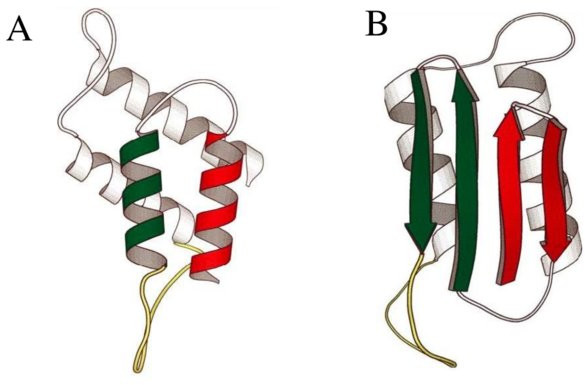
\includegraphics{images/PrPc.jpg}
	\caption{(A) Struttura della PrP$^{c}$. (B) Struttura della PrP$^{sc}$. Fonte: \cite{ruttkay2015prion}}
	\label{fig:PrPc}
\end{figure} 


\subsection{Controllo qualità e proteasomi}

L'uscita delle proteine dal reticolo endoplasmatico (RE) è controllata per assicurare la qualità delle proteine. Sebbene alcune proteine siano appositamente create e destinate a funzionare nel RE la maggior parte delle proteine che entrano nel RE sono destinate ad altri luoghi. Queste vengono impacchettate nelle vescicole di trasporto e gemmano per fondersi con l'apparato del Golgi. Ma l'uscita dal RE è altamente selettiva: le proteine che falliscono a ripiegarsi nella forma nativa e quelle che non si assemblano correttamente sono attivamente conservate nel RE attraverso i legami con i chaperoni molecolari che risiedono lì. Questi trattengono le proteine nel RE finché non si verifica il corretto ripiegamento o assemblaggio. Se questo non si verifica o fallisce ancora le proteine sono esportate nel citosol dove sono degradate da un \textit{proteasoma}. Le proteine da degradare sono contraddistinte dal loro legame con l'ubiquitina\footnote{Per "la scoperta della degradazione delle proteine mediata da ubiquitina" è stato assegnato il Premio Nobel per la chimica del 2004 ad Aaron Ciechanover, Avram Hershko ed Irwin Rose.}.

\par Ad esempio molecole di anticorpi sono composte da 4 catene polipeptidiche che si assemblano in completi anticorpi nel RE. Gli anticorpi parzialmente assemblati sono conservati nel RE finché tutte e 4 le catene non sono pronte. Le molecole di anticorpi che falliscono ad assemblarsi vengono degradate.

\par Nonostante l'indubbia utilità di questo meccanismo di controllo a volte questo può rivelarsi dannoso per l'organismo. Ad esempio la mutazione predominante che causa la \textit{fibrosi cistica}, comune malattia genetica che comporta seri danni polmonari, produce una proteina di trasporto della membrana plasmatica leggermente mal ripiegata. Tuttavia questa potrebbe funzionare normalmente se raggiungesse la membrana plasmatica ma viene bloccata nel RE e successivamente degradata\supercite{alberts2018essential} (per usare una metafora si può immaginare la situazione di un condannato alla pena di morte innocente). Le conseguenze sono terribili. La nota da sottolineare è che in questa malattia la mutazione non causa un'inattivazione di una proteina importante ma la proteina attiva è scartata dalle cellule prima che questa possa avere l'opportunità di funzionare. \\

\par I proteasomi sono complessi di \textit{proteasi} (enzima in grado di catalizzare la rottura del legame peptidico delle proteine) che degradano le proteine mal ripiegate attraverso reazioni di \textit{proteolisi}. Sono presenti nelle cellule di tutti gli eucarioti e procarioti. La struttura e la funzione di questi complessi è altamente conservata.

\par A causa del ruolo dei proteasomi nella regolazione del ciclo cellulare e dell'apoptosi\footnote{Il termine \textit{apoptosi} indica una forma di morte cellulare programmata (un'auto-distruzione). Al contrario della necrosi, che è una forma di morte cellulare risultante da un acuto stress o trauma cellulare, l'apoptosi è portata avanti in modo ordinato e regolato, richiede consumo di energia (ATP) e generalmente porta a un vantaggio durante il ciclo vitale dell'organismo (è infatti chiamata da alcuni morte altruista o morte pulita). Durante il suo sviluppo, ad esempio, l'embrione umano presenta gli abbozzi di mani e piedi “palmati”: affinché le dita si differenzino, è necessario che le cellule che costituiscono le membrane interdigitali muoiano}, sono oggi un bersaglio rilevante nelle terapie antitumorali. Farmaci inibitori nella terapia antiretrovirale interferiscono con il ciclo replicativo del virus HIV proprio bloccando l'attività dell'enzima della proteasi.


\subsection{Unfolded protein response}

La dimensione del RE è controllato dalla "richiesta" per il ripiegamento delle proteine. Il meccanismo di controllo nel RE, eseguito dai chaperoni molecolari, può essere sopraffatto. Quando succede le proteine mal ripiegate si accumulano nel RE. 
Se l'accumulo è abbastanza grande, questo innesca un complesso programma chiamato \textit{unfolded protein response} (UPR). Questo programma incita la cellula a produrre più RE, inclusi più chaperoni molecolari, e altre proteine riguardanti il controllo qualità. L'UPR permette alla cellula di regolare la dimensione del RE per gestire propriamente il volume delle proteine in entrata. In alcuni casi tuttavia anche un RE espanso non riesce a gestire la richiesta e l'UPR indirizza la cellula verso l'\textit{apoptosi}.

\par Una situazione del genere può avvenire negli adulti in cui insorge il diabete. I tessuti diventano gradualmente resistenti all'effetto dell'insulina. Per compensare questa resistenza le cellule che secernono insulina nel pancreas ne producono ancora di più. Si arriva infine alla situazione in cui il loro RE arriva ad una capacità massima e viene innescato l'UPR e di conseguenza la morte cellulare. Col tempo sempre più cellule secernenti insulina sono eliminate e la richiesta per quelle sopravvissute aumenta rendendole sempre più vulnerabili a questo meccanismo, esacerbando ulteriormente la malattia\supercite{alberts2018essential}.

\section{Eccezioni al postulato di Anfinsen}

-- IDP [ soft computing articolo]---
The structure of some proteins is difficult to determine
for a simple reason: A growing body of biochemical research
has revealed that a significant number of proteins, or regions
of proteins, do not have a distinct 3-D structure until they
interact with a target protein or other molecule. Their flexibil-
ity and indefinite structure are important for their function,
which may require binding with different targets at different
times. These proteins, which may account for 20–30% of
mammalian proteins, are called intrinsically disordered proteins
and are the focus of current research.


\subsection{Intrinsically disordered proteins}

\subsection{Fold switching proteins} \label{sec:fold-switching-proteins}
Some proteins have multiple native structures, and change their fold based on some external factors. For example, the KaiB protein complex switches fold throughout the day, acting as a clock for cyanobacteria. It has been estimated that around 0.5–4\% of PDB proteins switch folds.[7] The switching between alternative structures is driven by interactions of the protein with small ligands or other proteins, by chemical modifications (such as phosphorylation) or by changed environmental conditions, such as temperature, pH or membrane potential. Each alternative structure may either correspond to the global minimum of free energy of the protein at the given conditions or be kinetically trapped in a higher local minimum of free energy.[8]


--- porter, youtube ---
“I study proteins and proteins have been thought to have one structure that has one function or fold. I'm studying this group of proteins called fold switching proteins. So, they can actually change their structures and their functions in response to changes in the cell. So, you can kind of imagine fold switching proteins are like a transformer where in one case the protein is like a robot that does one thing and then in another case, in response to changes in our bodies, it becomes a car and can do something else. And an advantage to this is it can respond really quickly to changes in our bodies

\subsection{box: Filosofia della scienza}


\section{Il problema del Protein Folding}
• cos’è il problema del protein folding: non solo la struttura finale\\
• 3 sottoproblemi: folding code, protein structure prediction e folding process\\
• le domande di principio del protein folding\\
- paradosso di Levinthal

Come accennato nella sezione \ref{sec:assisted-folding}, la malattia di Alzheimer, la fibrosi cistica e altre malattie neurodegenerative sono associateal mal ripiegamento delle proteine. La conoscenza dei fattori di mal ripiegamento e la comprensione dei processo di ripiegamento proteico potrebero aiutare nello sviluppo di cure per queste malattie. La conoscenza della struttura delle proteine fornisce un grande vantaggio per lo sviluppo di nuovi farmaci e il design di nuove proteine.


\subsection{Limiti al ripiegamento}
• Limiti al ripiegamento: angoli di tersione e piano di Ramachandran\\

\subsection{Energetica del ripiegamento}
• processo spontaneo: energia di Gibbs, entalpia, entropia\\


--- Biochemists now know the amino acid sequence for about
160 million proteins, with about 4.5–5 million added each
month, and the three-dimensional shape for about 40,000.
Researchers have tried to correlate the primary structure of
many proteins with their three-dimensional structure to dis-
cover the rules of protein folding. Unfortunately, however,
the protein-folding process is not that simple. Most proteins
probably go through several intermediate structures on their
way to a stable shape, and looking at the mature structure
does not reveal the stages of folding required to achieve that
form

-- strumenti [ soft computing articolo]---
Even when scientists have a correctly folded protein in
hand, determining its exact three-dimensional structure is
not simple, for a single protein has thousands of atoms. The
method most commonly used to determine the 3-D structure
of a protein is X-ray crystallography


\clearpage
\chapter{Predizione della struttura di proteine (PSP)}

Il protein folding problem ha sia guidato che tratto beneficio dagli avanzamenti nei metodi sperimentali e computazionali\supercite{dill2008protein}. Uno dei maggiori obiettivi della biologia computazionale è proprio il PSP (Protein Structure Prediction), ovvero la predizione della struttura nativa tridimensionale di una proteina a partire dalla sua sequenza amminoacidica. Il PSP è il problema opposto al \textit{protein design} (la progettazione di nuove sequenze proteiche che abbiano delle specifiche attività).

\par Grazie al CASP, alla crescita del PDB e ai metodi per omologia veloce e di allineamento di sequenze i metodi computazionali hanno registrato notevoli progressi, come dimostra il livello raggiunto da AlphaFold. 

\par La predizione della struttura di proteine è uno strumento fondamentale in medicina per la comprensione delle malattie da misfolding, nell'industria farmaceutica per risparmiare anni di laboriosi e costosi esperimenti correntemente richiesti per lo sviluppo di un singolo farmaco (\textit{drug design}), in biotecnologia per il design di nuovi enzimi e in generale per acquisire maggior conoscenza sul protein folding in tutti i suoi lati.

\par I biochimici conoscono oggi la sequenza amminoacidica per più di 225 milioni di proteine\supercite{proteienDBentries} (UniProt), con circa 4.5-5 milioni aggiunte ogni mese. La struttura tridimensionale è conosciuta per circa 160.000 proteine\supercite{proteienDBentries} (PDB)\footnote{Al 3 Febbraio 2022 sono presenti 162.913 strutture di proteine nella versione dell'RCSB. Nel PDB ci sono anche strutture di altre macromolecole (complessi di acidi proteici-nucleici, DNA e RNA) per un totale, incluse le proteine, di 186670\supercite{pdbStats}. Nel wwPDB (database globale) vi sono in totale 197961 strutture di macromolecole\supercite{wwpdbStats}.} con più di 10.000 strutture aggiunte ogni anno. 

\begin{figure}[!htb]
	\centering
	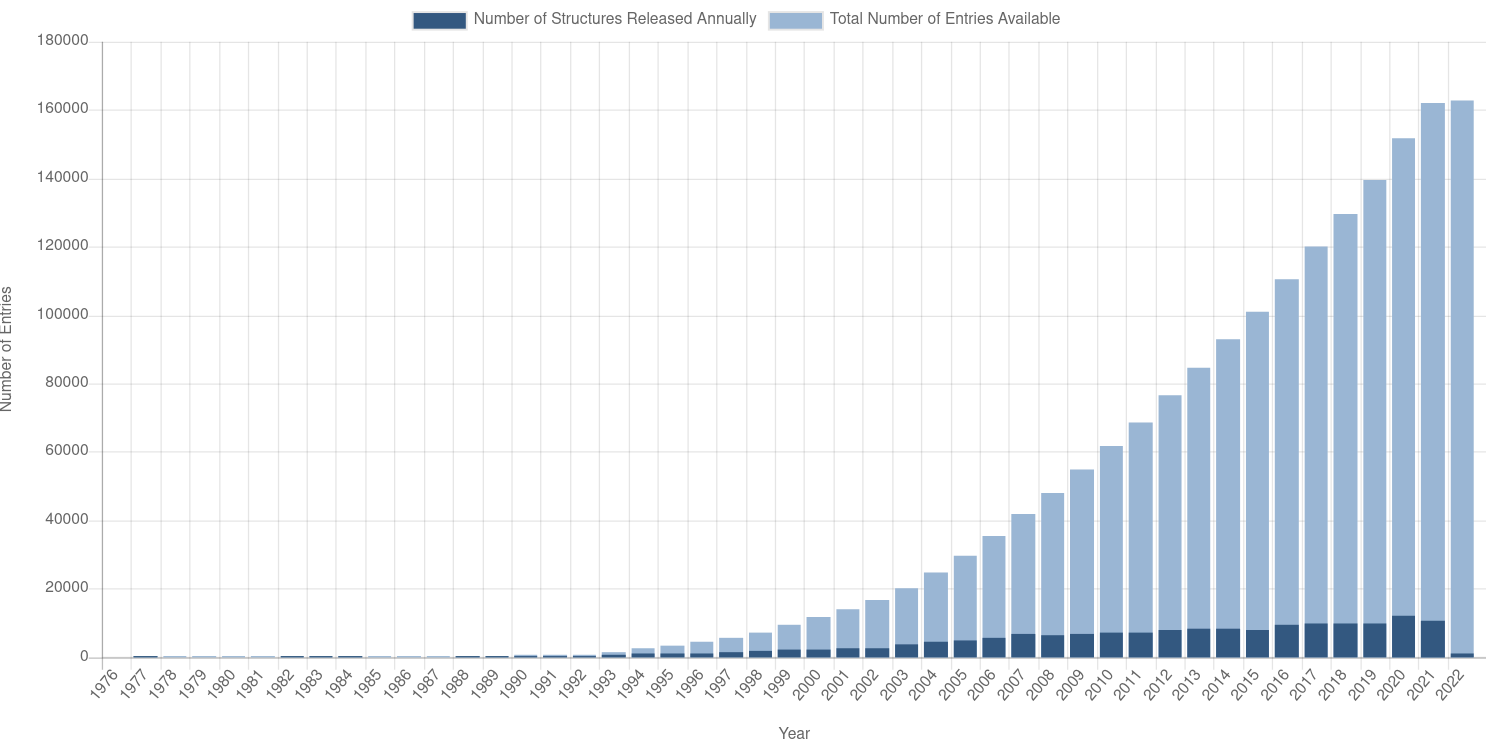
\includegraphics[scale=0.3]{images/pdb-statistica.png}
	\caption{Crescita complessiva del numero di strutture di proteine pubblicate nel PDB. Fonte\cite{pdbStats}}
	\label{fig:pdb-statistica}
\end{figure}


\section{Determinazione sperimentale} \label{sec:experimentally-guided-prediction}

La determinazione sperimentale della struttura delle proteine ha vissuto dei progressi significativi col passare degli anni ed è di grande importanza per i metodi computazionali di PSP.


- come le proteine sono studiate [alberts, 4.4 p.158]
- metodi sperimentali 
alberts p.168
pal 6 p.126 ma è molto tecnico
wiki-protein folding, 
baxevanis 12 p.363

• storia dei metodi sperimentali (Pal) \\
• cristallografia a raggi-x \\
• NMR, risonanza magnetica nucleare \\
• Cryo-EM (electron microscopy) \\
\subsection{Predizione guidata sperimentalmente}
kessel 3.5
pal 6.2.5 p.138

Anche quando gli scienziati hanno una proteina correttamente ripiegata fra le mani non è così semplice determinarne la sua esatta conformazione tridimensionale, considerando che si parla di strutture di migliaia di atomi.

 Integrating experimental (i.e., lab) data with predictions [235]. Low-resolution
methods for the determination of protein structures (e.g., electron microscopy) have
recently been used for deriving geometric constraints, which can be applied along
with computational methods to achieve better predictions.

\section{Strumenti e metodi informatici}
La piccola percentuale di strutture determinate e il gap che continua a crescere con le sequenze conosciute è una conseguenza della lentezza dei metodi sperimentali (e in parte dei progressi delle tecnologie di sequenziamento). I metodi computazionali, significativamente più veloci ed economici, potrebbero risolvere (almeno parzialmente) questo problema.

\subsection{Paradigmi per approssimazione biologica}
kessel 3.4 [computational methods for structure prediction]
pal 15.3.2 Computational structure prediction. Molto breve
pal 18.1 [molecular dynamics]
psp-wiki [abbastanza discorsivo]
prot-eng-wiki[molto breve]
Gu 28-33 [serie di articoli messi insieme, sembra stra interessante]
baxevanis 12 p.385 \\ \\


I numerosi metodi computazionali per il PSP possono essere suddivsi in base ai due diversi macro-approcci utilizzati\footnote{Le sezioni sui paradigmi per approssimazione biologica seguono e si basano sul capitolo 3.4 di \fullcite{kessel_ben-tal_2018}}:
\begin{itemize}
	\item \textit{ab initio} (o \textit{de novo}), approccio fisico, nei quali la struttura è predetta da zero usando principi fisici
	\item \textit{template-based}, dove vengono usate informazioni da strutture 3D note di proteine. Questo approccio è ulteriormente divisibile in:
	\begin{itemize}
		\item \textit{homology modeling}, basato su confronti sequenza-sequenza tra la proteina da predire e il modello
		\item \textit{fold recognition}, basato su altre similitudini fra modello e proteina da predire
	\end{itemize}
	\item ?? \textit{covariazione evolutiva}, ??
\end{itemize}


\subsection{Rappresentazione informazioni}
pal 6.4.1 p.145
Gu 10-13 p.468
baxevanis 12 p.367

\subsection{Database}
baxevanis 12 p.373, 1

\subsection{Visualizzazione proteine}
pal 6.4 p.146, ottima
kessel p.174 (2.3 GRAPHIC REPRESENTATIONS OF PROTEINS)

\subsection{CASP}

\section{Workflow PSP}
- paper Soft computing
- wiki psp

\subsection{Input, output, valutazione}
\subsubsection{Proprietà dei dati di input}

\subsubsection{Output: modelli, ... [..]}
\subsubsection{Metriche di valutazione}
- Gu 16 p.655 GENERAL APPROACH TO STRUCTURE COMPARISON AND ALIGNMENT
baxevanis 12 p.386


\section{Approccio \textit{ab initio}}
{
Il metodo più lineare e a prima vista ovvio per predire la struttura nativa di proteine è seguire la natura, simulando accuratamente come le forze fisiche guidino la proteina a ripiegarsi e usare questa simulazione per riprodurre il processo di ripiegamento su proteine con strutture sconosciute. \textit{Ab initio}, termine latino, significa infatti "dall'inizio".

\par Il primo problema che sorge è superare il paradosso di Levinthal. Per farlo si assume un profilo energetico a imbuto del ripiegamento, ovvero la premessa termodinamica che la forma nativa di una proteina sia lo stato in cui risulta avere più bassa energia libera, o più precisamente (richiamando la definizione di struttura nativa data nella sez. \ref{sec:energetica}) quella conformazione avente minore energia libera tale da mantenere il livello di dinamicità richiesto alla proteina per svolgere la sua funzione biologica.

\par Le predizioni nell'approccio \textit{ab initio} sono pertanto \textit{energy-based}. In quanto tali usano solo informazioni sul tipo di atomi nel sistema, le loro posizioni relative nello spazio tridimensionale e le loro interazioni con gli altri atomi. Viene poi calcolato l'intero contenuto di energia del sistema e le forze agenti su ogni atomo. 

\par L'energia totale di un sistema (\textit{free energy}) può essere decomposta in varie componenti: cinetica, potenziale, termica ecc. È l'energia libera che determina la stabilità del sistema. Come si vedrà sotto, nell'approccio fisico non viene calcolata tutta l'energia libera ma solamente approssimata con una parte di essa per motivi di complessità.

\par Sebbene vi siano differenti metodi in questo approccio, tutti condividono due caratteristiche di base:
\begin{itemize}
	\item calcolano il contenuto di energia del sistema in una singola configurazione
	\item campionano numerose configurazioni e ne trovano una con la minor energia libera
\end{itemize}

Per \textit{configurazione} si intende la disposizione complessiva di tutti gli atomi di tutti i componenti del sistema (proteina, solvente, ioni, membrana ecc.) mentre la posizione collettiva dei soli atomi della proteina viene chiamata \textit{conformazione}.

\subsection{Molecular mechanics \& dynamics}

\par Per descrivere in maniera affidabile tutte le forze fisiche operanti sul sistema tra i differenti atomi bisognerebbe descriverne la distribuzione di tutti gli elettroni, il che richiede però calcoli di meccanica quantistica (QM). Le forze, in un sistema molecolare, risultano dalla distribuzione spaziale degli elettroni attorno agli atomi. Sfortunatamente questi calcoli sono computazionalmente molto costosi e una rigorosa caratterizzazione di un sistema macromolecolare, con milioni di atomi, è al momento insostenibile. Calcoli di QM su una singola conformazione di una piccola proteina possono richiedere mesi, tempi troppo lunghi se si ha l'obiettivo di provare tante configurazioni per sceglierne una finale. 

\subsubsection{Molecular mechanics}

\par Per le ragioni sopra elencate gli scienziati spesso investigano sistemi macromolecolari usando approssimazioni delle reali forze in essi. Il campo da cui i calcoli per le approssimazioni sono presi è chiamato \textit{molecular mechanics} (MM), poiché approssima sistemi molecolari usando espressioni prese dalla meccanica newtoniana classica:
\begin{itemize}
	\item il contenuto di energia è descritto usando un \textit{campo di forza} nel quale gli atomi e i legami covalenti sono trattati come palline e molle
	\item le descrizioni che richiederebbero calcoli di QM vengono ignorate
	\item le rappresentazioni sono \textit{esplicite}: prendono in considerazione tutti gli atomi (vedi fig. \ref{fig:descrizione-esplicita-mm})
\end{itemize}

Il campo di forza sopra accennato descrive l'energia potenziale del sistema. Da notare che l'energia potenziale (intesa come entalpia) è solo una delle due componenti dell'energia libera, vedi sez. \ref{sec:energetica}).

\par Un campo di forza è un'energia di posizione: l'energia di un oggetto in una specifica posizione all'interno di un campo (gravitazionale, elettrico, magnetico ecc.). Nelle molecole l'energia potenziale è la somma di tutti gli effetti dei campi elettrici atomici\footnote{gli atomi possiedono, in base alla loro eventuale carica, campi elettrici che influenzano gli altri atomi} in una determinata posizione. Si può approssimare l'energia potenziale all'energia risultante da tutti i legami covalenti e le interazioni non covalenti, escluse quelle non polari \footnote{un esempio di interazione non polare è l'effetto idrofobico. Vengono escluse poiché coinvolgono principalmente cambiamenti di entropia nel solvente}, in una singola configurazione del sistema.

\begin{figure}[!htb]
	\centering
	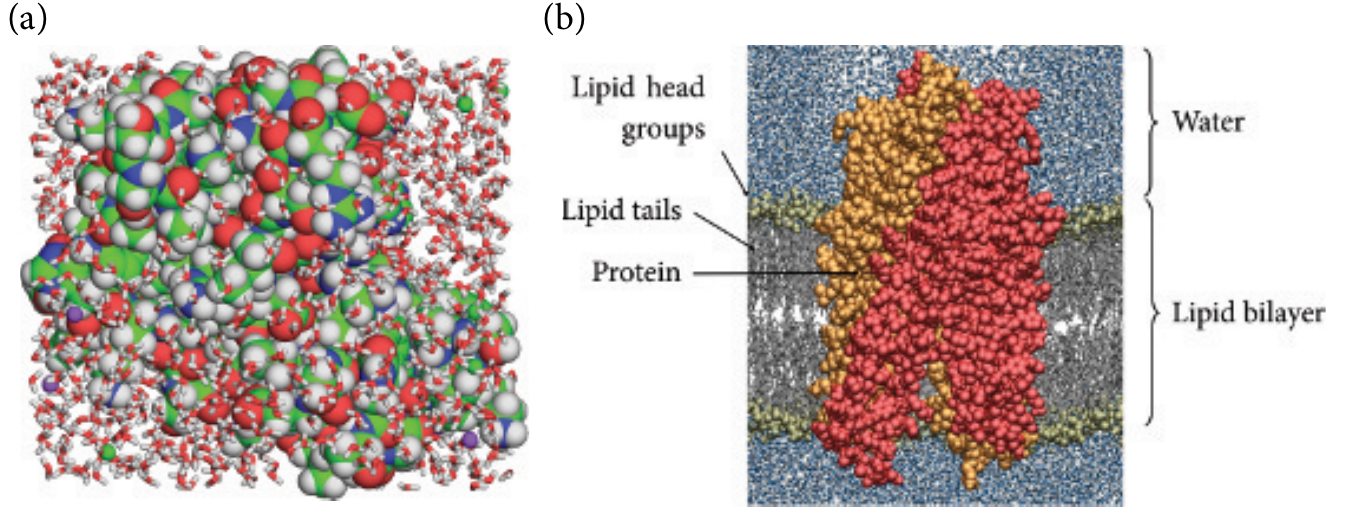
\includegraphics[scale=0.4]{images/esplicita-mm.png}
	\caption{Descrizioni esplicite nei calcoli di MM. (A) una piccola proteina immersa in un solvente composto da molecole d'acqua e ioni (Na$^{+}$, Cl$^{-}$). La proteina è rappresentata come sfere di atomi, l'acqua come bastoncini e gli ioni come piccole sfere magenta e gialle. (B) una proteina trasportatrice in un doppio strato lipidico, circondato da ambiente acquoso. La proteina e le teste dei lipidi sono rappresentate in modo space-fill, mentre l'acqua e le code dei lipidi con rappresentazione wire-frame. Fonte \cite{kessel_ben-tal_2018}}
	\label{fig:descrizione-esplicita-mm}
\end{figure}

\par La descrizione approssimata fornita dal campo di forza permette di calcolare l'energia potenziale di molti sistemi macromolecolari in meno di un secondo. \\

\par Una variante del MM è la \textit{QM/MM} nella quale i calcoli di QM sono indirizzati solamente su una piccola parte della proteina che contiene residui funzionali importanti. Le altre regioni sono soggette invece a MM, con calcoli molto più veloci \footnote{questo approccio è stato introdotto da Warshel, Levitt e Karplus}

\subsubsection{Spazio configurazionale}

\par Assumendo l'accuratezza del campo di forza, il calcolo dell'energia potenziale di un sistema consente di determinare (parte del)la stabilità di una configurazione. L'idea iniziale potrebbe essere quella di considerare tutte le possibili locazioni atomiche del sistema, calcolare l'energia potenziale in ogni caso e scegliere quella con la minor energia. Come si può facilmente intuire ciò risulta essere un procedimento troppo oneroso, in quanto si devono considerare anche gli atomi del solvente (ed eventuali ligandi o cofattori). Anche il solo numero delle possibili configurazioni atomiche è difficile da calcolare.

\par Per superare questo problema vengono usate tecniche per ridurre lo spazio di ricerca nello spazio configurazionale. Ci sono vari metodi di ricerca, ad esempio: \textit{systematic search }(grid search basata su dettagli geometrici), \textit{model-building model }(usa frammenti molecolari), \textit{random approach }(movimenti random sul piano cartesiano da una configurazione iniziale), \textit{distance geometry} (usa una matrice di distanze atomiche), \textit{Monte Carlo method} (modifiche random e accettazione probabilistica di configurazioni a livelli energetici maggiori)\supercite{ROY2015151}.

\par Il metodo più semplice è chiamato \textit{energy minimization}:

\begin{enumerate}
	\item si parte da una configurazione arbitraria
	\item si calcola l'energia potenziale. Viene derivato questo valore su differenti posizioni nel sistema in modo da calcolare le forze agenti su ogni atomo dalla rimanente parte del sistema
	\item un piccolo cambiamento è introdotto nella posizione di ogni atomo, in risposta alle forze applicate su ognuno di essi dal resto del sistema (in accordo a quanto calcolato nel precedente step)
	\item se la nuova configurazione ha un'energia minore viene adottata
	\item altrimenti questa viene scartata e viene creata una nuova configurazione
	\item si ritorna allo step 3 finché non si trovano più configurazioni con minor energia
\end{enumerate}

Il metodo passa da una configurazione all'altra scendendo con il gradiente della superficie dell'energia potenziale finché non converge in un \textit{punto di minimo locale}. Tutte le procedure di \textit{energy minimization }tendono a rimanere bloccate in un minimo locale di energia non riuscendo spesso a raggiungere il minimo globale a causa di \textit{barriere energetiche} da scavalcare per raggiungere una configurazione con energia minore (vedi fig. \ref{fig:energy-minimization} e \ref{fig:imbuto}).

\begin{figure}[!htb]
	\centering
	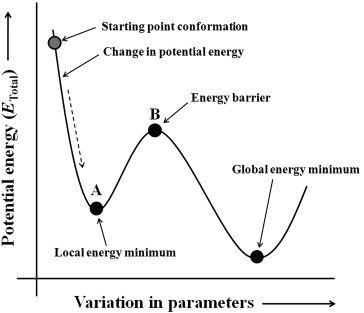
\includegraphics[scale=1]{images/energy-minimzation.jpg}
	\caption{Differenti fasi energetiche di una molecola durante la sua minimizzazione energetica. Fonte\cite{ROY2015151}}
	\label{fig:energy-minimization}
\end{figure}

\subsubsection{Molecular dynamics}

È possibile spingere l'algoritmo di minimizzazione energetica fuori da punti di minimo locale fornendo energia extra, ad esempio innalzando la temperatura del sistema (ovvero aggiungendo calore virtuale). L'energia aggiunta consente agli atomi del sistema di incrementare i loro movimenti e nuove configurazioni fuori dalle barriere energetiche vengono create. Questo metodo è chiamato \textit{Molecular dynamics} (MD) e si focalizza sui movimenti dipendenti dal tempo degli atomi nel sistema. I calcoli sono realizzati in accordo alla meccanica classica. 

\par Agli atomi viene assegnata una velocità iniziale (proporzionale alla temperatura) e continuano a muoversi nello spazio secondo i corrispondenti cambiamenti nell'energia potenziale del sistema. Il movimento di ogni atomo nel sistema è calcolato in base alla sua energia in quel dato momento.

\par Le simulazione di MD sono eseguite in cicli ripetitivi di \textit{riscaldamento} e \textit{raffreddamento} (metodo conosciuto nel mondo informatico come \textit{simulated annealing}, in riferimento al processo di tempra dei metalli). Nella fase di riscaldamento vengono superate le barriere energetiche mentre la fase di raffreddamento (seguita dall'\textit{energy minimization}) consente al sistema di rilassarsi in configurazioni con minor energia.

\par Un metodo comune per rendere la ricerca con MD più efficiente è di spezzarla in due fasi:
\begin{itemize}
	\item ricerca a bassa risoluzione per trovare una collezione di strutture con interazioni non polari (basato sulla nozione che il nucleo delle proteine globulari sia idrofobico)
	\item ricerca ad alta risoluzione fra le strutture selezionate nel primo step
\end{itemize}

\subsubsection{Limiti dell'approccio fisico e parziali soluzioni}
I metodi di MM/MD trovano difficilmente impiego in processi biologici rilevanti come il protein folding.
Alcuni problemi riguardano l'approssimazione in sé del campo di forza, la sua accuratezza e i possibili doppi conteggi delle forze in gioco (es. interazioni ioniche e legami idrogeno calcolate in due espressioni differenti). 

\par Un altro problema, sempre nell'approssimazione dell'energia libera con campi di forza, è che forniscono sì l'energia potenziale ma non l'entropia. L'unico modo per stimare l'entropia e l'energia libera dai calcoli per l'energia potenziale è eseguire questi calcoli su tutte le possibili configurazioni del sistema e poi integrarli. Il problema risiede quindi nell'impossibilità di compiere la totalità di questi calcoli a causa delle rappresentazioni esplicite usate nelle simulazioni di MD. In particolare è difficile considerare tutte le configurazioni del solvente acquoso. Ciò che si sta calcolando non è l'energia libera ma un \textit{potenziale di forze medie} (PMF). In conclusione le simulazioni di MD non sono consigliate per descrivere gli effetti dei solventi.

\subsection{Limiti e utilità}

\subsubsection{Mean field approach}
Per ovviare parzialmente al problema delle rappresentazioni esplicite è possibile descrivere \textit{implicitamente} parti del sistema che vengono descritte da una proprietà media, per questa ragione tale approccio è chiamato \textit{mean field}. Un esempio è la descrizione del solvente, la parte "meno" interessante in genere, come una massa omogenea descritta dalla sua \textit{dielettricità} \footnote{proprietà di un mezzo non conduttore di essere sede di un campo elettrostatico}, conosciuto anche come approccio \textit{continuum-solvent}, vedi fig. \ref{fig:mean-field}.

\begin{figure}[!htb]
	\centering
	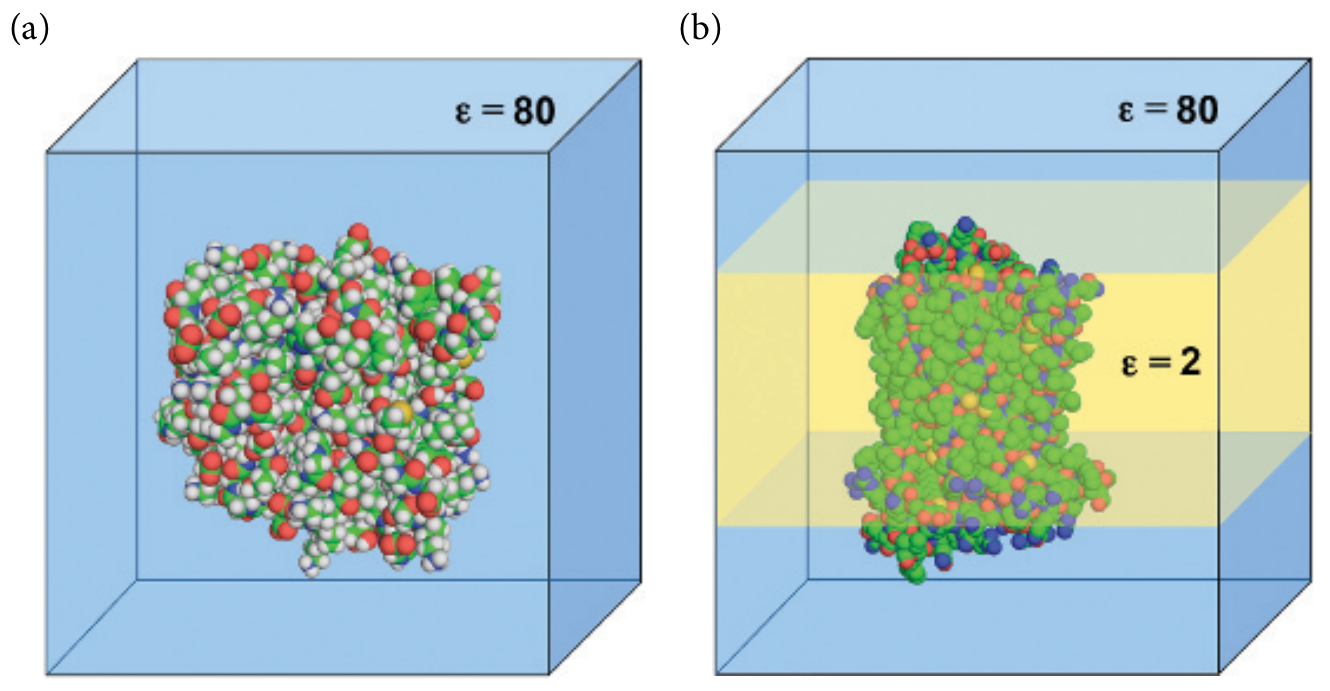
\includegraphics[scale=0.4]{images/mean-field.png}
	\caption{Descrizione con approccio mean-field di un sistema, il solvente è descritto implicitamente mentre la proteina esplicitamente. $\epsilon$ indica la dielettricità. (A) proteina in un solvente acquoso altamente dielettrico. (B) proteina di membrana in un ambiente eterogeneo. Il solvente acquoso è altamente dielettrico mentre la lastra semi-trasparente gialla, che rappresenta la regione biologica di doppio strato lipidico, è poco dielettrica. Fonte\cite{kessel_ben-tal_2018}}
	\label{fig:mean-field}
\end{figure}

Ovviamente, essendo una forte approssimazione, alcuni aspetti del sistema reale sono ignorati, come le interazioni fra gli atomi delle proteine e le molecole d'acqua. Tale problema si esacerba quando il solvente è una membrana. \\

\par Un altro compromesso è l'approccio \textit{mixed force fields} che combina calcoli espliciti sulla proteina e calcoli impliciti sul solvente. Viene usata l'equazione di Poisson-Boltzman (PBE) per calcolare accuratamente l'energia libera elettrostatica, legando così l'effetto polarizzante delle cariche con il loro ambiente. Essendo però un calcolo oneroso viene in genere risolta l'equazione generalizzata di Born (GB). A partire da queste due equazioni, che calcolano la componente elettrostatica dell'energia libera, è possibile calcolare l'intera \textit{free energy}, in modo abbastanza accurato, con calcoli che si rifanno alla surface area (SA, vedi parte finale della sez. \ref{sec:termodinamica-forze-idrofobiche}). 

\par Questi metodi sono chiamati \textit{PBSA} e \textit{GBSA} rispettivamente, e come si è visto permettono un calcolo più preciso dell'energia libera. Questi possono a loro volta essere combinati con la MM per rappresentare anche le interazioni del sistema (\textit{MM-PBSA, MM-GBSA}) e sono oggi largamente utilizzati.

\par Un altro limite computazionale è il lasso temporale che si riesce a coprire. La maggior parte delle proteine si ripiega in microsecondi mentre le simulazioni riescono a coprire tempi che vanno dai pico ai nanosecondi. Grazie ad avanzamenti nelle risorse informatiche sono stati fatti dei passi avanti da questo punto di vista. Un caso interessante è \textit{Anton}, un supercomputer progettato specificatamente per ottimizzare simulazioni di MD capace di coprire 85$\mu s$ al giorno per un sistema molecolare di 23.000 atomi (180 volte più veloce di qualsiasi computer general-purpose). Altri progressi sono dovuti alla computazione parallela e alla computazione accelerata dalla GPU. Il calcolo distribuito (\textit{grid computing}), ovvero una larga rete di computer personali dedicati volontariamente al completamento di processi, ha permesso alla rete \textit{Folding@Home} (170.000 computer) di simulare l'intero processo di ripiegamento della proteina di legame dell'acetil coenzima A, composta da 86 residui e che richiede 10 millisecondi per ripiegarsi. Un'altra rete distribuita di calcolo è \textit{Rosetta@Home}, con 86.000 nodi e finalizzata al PSP. \\

\par Un possibile metodo di azione è la \textit{frammentazione delle proteine}, nel quale i calcoli sono realizzati su piccoli frammenti della proteina e poi integrati. Un esempio è il software QUARK. L'approccio \textit{fragment-based} è usato nei metodi che combinano predizioni \textit{template-based} con assemblaggi \textit{ab initio}.

\subsubsection{Conclusioni sull'approccio \textit{ab initio}}
Gli approcci \textit{ab initio} non sono attualmente in grado di predire la struttura della maggior parte delle proteine sulla sola base della loro sequenza. Ma sono molto abili nel farlo quando il punto di partenza della predizione è una struttura vicino a quella nativa. Questi metodi sono infatti ampiamente usati per raffinare le strutture grezze ottenute dalle determinazioni sperimentali (vedi sez. \ref{sec:experimentally-guided-prediction}). Hanno anche fornito informazioni importanti sulla dinamica delle proteine e sono utilizzati anche nel \textit{protein engineering} e nel \textit{drug discovery}.

}

\section{Approccio \textit{template-based}}
Le proteine che esistono in natura oggi si sono sviluppate attraverso lunghi processi evoluzionistici, progredendo attraverso mutazioni casuali e selezione naturale. La rivoluzione genetica degli anni '50, consentendo la determinazione delle sequenze amminoacidiche, ha permesso il nascere di metodi di confronto delle sequenze. Si possono ricavare informazioni sulla struttura 3D delle proteine cercando altre proteine con proprietà nella sequenza simili e una struttura nota, ovvero dei \textit{template}. 

\subsection{Homology modeling}
Nella modellazione per omologia ci si affida a somiglianze nella sequenza tra la proteina target e i template. I metodi per omologia sono perciò basati sul paradigma: \\
 \say{\textit{la sequenza codifica per la struttura}}.

\par Sono metodi basati anche sull'osservazione che la struttura terziaria è più conservata della sequenza amminoacidica. Di conseguenza ci si aspetta una significativa somiglianza nella struttura fra proteine che condividono una notevole somiglianza tra le sequenze, anche non totale.

\par In altri termini, due sequenze amminoacidiche molto simili (\textit{omologhe}) , in due proteine differenti ma evoluzionisticamente collegate, dovrebbero acquisire la stessa struttura locale.

\par La modellazione per omologia consiste tipicamente nei seguenti passi:
\begin{enumerate}
	\item ricerca e selezione del template
	\item costruire un MSA (Multiple Sequence Alignment) che includa la proteina target e i template
	\item assegnare le coordinate spaziali dei template alla sequenza della proteina target
	\item raffinamento della struttura modello
	\item valutazione e validazione della struttura risultante
\end{enumerate}

\begin{figure}[!htb]
	\minipage{0.48\textwidth}
	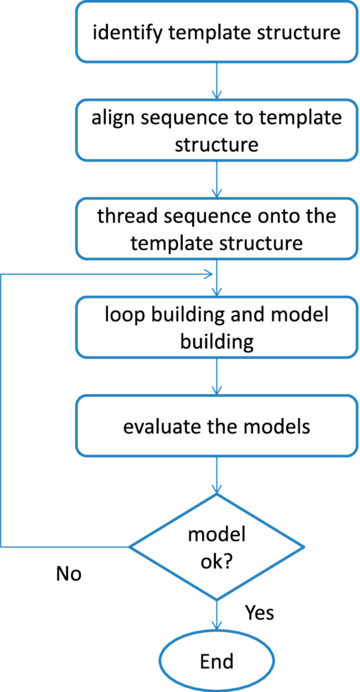
\includegraphics[scale=0.43]{images/homology1.png}
	\caption{Diagramma di flusso della modellazione per omologia. Fonte: \cite{sliwoski2014computational}}
	\label{fig:omologia-flusso}
	\endminipage\hfill
	\minipage{0.48\textwidth}
	\centering
	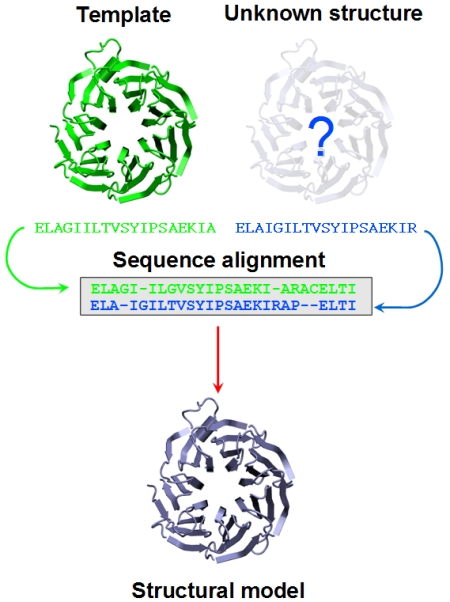
\includegraphics[scale=0.5]{images/homology2.jpg}
	\caption{Schema esemplificativo di una modellazione per omologia. Fonte \cite{UNIL-homology}}
	\label{fig:omologia-esempio}
	\endminipage\hfill
\end{figure}

Nel 1° step si cerca una struttura modello, almeno una, tra le strutture conosciute avente un'alta somiglianza di sequenza. È più semplice se la struttura di un una proteina omologa molto simile è stata già risolta. Ci sono però altri gruppi di proteine, come le proteine di membrana, le cui strutture risolte sono scarse. Trovare i giusti template e caratterizzare la loro omologia è ciò che determina in genere il successo dell'intera predizione (una somiglianza minore del 30\% avrà risultati molto scarsi, mentre sopra al 50\% la predizione ha buona probabilità di essere di buon livello). È possibile in ogni caso che vi sia una somiglianza \textit{locale} anche quando la somiglianza globale è scarsa. Alcuni algoritmi noti per trovare template sono PSI-BLAST e HMM (Hidden Markov Models), quest'ultimo molto usato.

\par Nel 2° step vengono sfruttate informazioni evoluzionistiche per migliorare l'allineamento tra le sequenze dei template e del target. È difficile stabilire allineamenti fra omologhi distanti, come nel caso di target \textit{e} e template \textit{procarioti}. Ci sono vari tool per creare MSA, ad esempio: Clustal$\Omega$, MAFFT, MUSCLE, T-Coffee. Possono venire utilizzati più MSA insieme per sopperire a problemi di disallineamento di piccole regioni. Il MSA viene illsutrato nella sezione \ref{sec:MSA}.

\par Nel 3° step ad ogni segmento della sequenza target viene assegnato un insieme di coordinate spaziali in accordo ai risultati del MSA. Tool noti sono MODELLER, NEST e SWISS-Model. La struttura ottenuta potrebbe essere però deformata a causa dell'utilizzo di più template e numerosi inserzioni e cancellazioni. Possono essere presenti lunghezze e angoli dei legami non ottimali e atomi sovrapposti.

\par Per ovviare a tali problemi nello step 4 si applica un processo di raffinamento, specialmente per quanto riguarda i loop (vedi sez. \ref{sec: loop-modeling}), regioni fodamentali per i siti di legame. Vengono applicati algoritmi che confrontano caratteristiche geometriche ed effettuano calcoli energetici che identificano configurazioni atomiche sfavorevoli. 

\par Nel 5° step si valuta l'affidabilità della predizione in vari modi:
\begin{itemize}
	\item alcune qualità della struttura costruita possono essere confrontate con delle tendenze statistiche
	\item se ci sono vari modelli predetti si calcola l'energia libera e si sceglie la struttura con minor energia libera
	\item la conservazione evoluzionistica a livello amminoacidico può essere correlata con il loro stato "esposto" o "seppellito" (l'idea di partenza è che il nucleo della proteina rimanga inalterato e la superficie sia variabile)
	\item se si hanno a disposizione dati sperimentali della struttura nativa della proteina si può validare il modello con la consistenza a essi.
\end{itemize}

\subsubsection{Efficienza e limiti}

Con una somiglianza maggiore del 50\% si registra una r.m.s.d. che tra 1 e 2 \angstrom, ma è importante notare che non sempre proteine omologhe (vicine sequenzialmente) condividono la stessa funzione e struttura. Un esempio sono le proteine del lievito Gal1 e Gal3: 73\% di identità e 92\% di somiglianza. Queste due proteine hanno però sviluppato differenti funzioni, con Gal1 che è una galattochinasi mentre Gal3 è un induttore trascrizionale\supercite{platt2000insertion}.

\par Non c'è quindi una soglia che assicuri una sicura predizione della struttura: molte proteine con una lontana somiglianza possono svolgere la stessa funzione mentre altre altamente simili possono svolgere funzioni diverse. Una regola empirica è considerare sequenze con più del 30-40\% di somiglianza come sequenze con una struttura o funzione simile.

\begin{figure}[!htb]
	\centering
	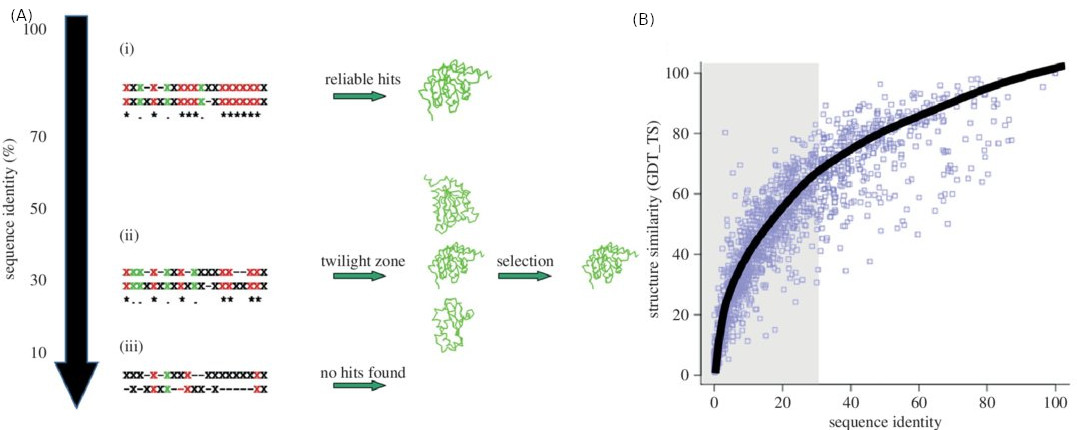
\includegraphics[scale=1.2]{images/homology-grafico.jpg}
	\caption{Risultati dei metodi per omologia alla variazione dell'identità nella sequenza. (A) Dimostrazione schematica dell'uso di confronti di sequenze per identificare omologie strutturali. 'X' indica un qualsiasi amminoacido. (i) identità > 70\%: semplici allineamenti di sequenza sono sufficienti per trovare il corretto ripiegamento. (ii) Tra il 20 e il 30\% non sempre è possibile trovare il corretto ripiegamento; è necessario effettuare ulteriori raffinamenti. (iii) a bassi livelli l'utilità di questo metodo è molto bassa. (B) Somiglianza strutturale (in GDT\_TS score) al variare dell'identità della sequenza. Anche al 30\% il livello di somiglianza è significativo. Fonte\cite{joseph2014local}}
	\label{fig:omologia-grafico}
\end{figure}

\par Un'osservazione fondamentale risiede sulle basi in sé del metodo: dato l'affidamento pressoché totale nella modellazione comparativa, la struttura modello è condizionata necessariamente a essere più simile ai template che alla reale struttura nativa della sequenza target, nonostante i vari processi successivi di raffinamento che, data la loro natura approssimativa, non sono perfetti. 

\par I problemi maggiori risultano nelle regioni con bassa somiglianza, come ci si può aspettare. Si sta parlando specialmente dei \textit{loop}, soggetti a mutazioni considerevoli durante l'evoluzione.

\par Si incorrono in problemi con la modellazione per omologia quando si trattano proteine che non hanno omologhe tra le strutture conosciute, come le proteine di membrana, le quali sono difficili da da cristallizzare. \\

\subsubsection{Conclusioni sull'approccio \textit{template-based}}

\par Nonostante tutte le osservazioni fatte, \textit{la modellazione per omologia è correntemente il miglior metodo computazionale per predire la struttura delle proteine} e la sua applicabilità è destinata a crescere con l'aggiunta di nuove strutture determinate sperimentalmente da poter essere usate come template.

\par La sfida principale che questi metodi hanno affrontato, e che AlphaFold ha "vinto", era raggiungere almeno una r.m.s.d. di 3\angstrom. Le sfide ancora da superare riguardano l'accuratezza su grandi proteine, su proteine con un contenuto significativo di strutture $\beta$ e la modellazione di proteine multi-dominio e di membrana.

\par Oltre alla PSP i metodi per omologia sono anche usati nel drug design (per studiare le differenze strutturali fra le proteine bersagliate dallo stesso farmaco) e nello studio dei meccanismi catalitici.

\subsection{Loop modeling} \label{sec: loop-modeling}
- karami 2019
- rosetta
- wiki

\subsection{Sequence alignment} \label{sec:MSA}
- protein sequence alignment (poi MSA)
[Burkowski 6 p.167]
baxevanis 8 p.227


Certain software programs can display multiple sequences together to show the degree of similarity between them

This is called a sequence alignment and is commonly used to show the degree of relatedness between sequences

Le sequence di proteine in genere risultano avere un grado di somiglianza maggiore rispetto alle sequenze nucleotidiche, questo è dovuto alla degenerazione del codice genetico e al fatto che quasi per ogni amminoacido esistono vari codoni che lo codificano, perciò differenti sequenze nucleotidiche possono codificare esattamente la stessa sequenze di amminoacidi.

\begin{figure}[!htb]
	\centering
	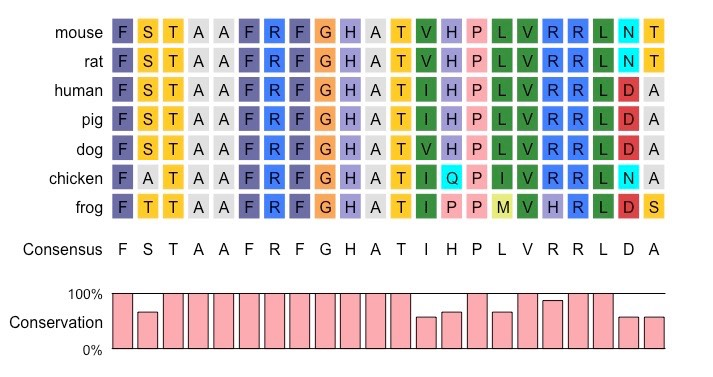
\includegraphics[scale=0.5]{images/msa.jpeg}
	\caption{Multiple sequence alignment schematica di una sequenza proteica di varie specie. Fonte\cite{msaBioNinja}}
	\label{fig:msa}
\end{figure}

\subsection{Fold recognition via threading}
- praveen 2014
- pal 

Nei metodi per \textit{fold recognition} ci si basa su somiglianze nelle inclinazioni derivate dalla sequenza, come la formazione di strutture secondarie, o su tendenze statistiche.

\begin{figure}[!htb]
	\centering
	\includegraphics[scale=0.53]{images/threading-mappa.png}
	\caption{. Fonte\cite{joseph2014local}}
	\label{fig:fold-recognition}
\end{figure}

\section{Approccio per \textit{covariazione evolutiva}}



L'approccio per coevoluzione evolutiva può essere combinato con l'approccio \textit{template-based}, come dimostra AWSEM\supercite{jin2020protein} nella 13° edizione del CASP, il quale contiene anche metodi di ottimizzazione di energia e utilizzo di reti neurali.


\section{Predizione della struttura secondaria}


\section{Metodi integrativi}

- predictive methods
baxevanis 7

\subsection{Case study: \textit{TASSER}}

\subsection{Case study: \textit{ROSETTA??}}

\subsection{Macromolecular docking??}

\section{Protein Function Prediction}
- pfp wiki

One should remember, though, that effi-
cient protein structure prediction is just a means to an end; the real challenge of structural
biology has always been (and still is) to deduce the functions of proteins on the basis of their
sequences and/or structural data [190].

Knowing the structure of a protein often allows functional prediction as well.

There is no hard sequence-similarity threshold for "safe" function prediction; many proteins of barely
detectable sequence similarity have the same function while others (such as Gal1 and Gal3) are highly
similar but have evolved different functions. 

For enzymes, predictions of specific functions are especially difficult, as they only need a few key residues
in their active site, hence very different sequences can have very similar activities. By contrast, even with
sequence identity of 70\% or greater, 10\% of any pair of enzymes have different substrates; and differences
in the actual enzymatic reactions are not uncommon near 50\% sequence identity.

\section{Paradigmi nel soft computing}
\subsection{ANN, EC, SVM, .. [..]}
\subsection{altri approcci [..]}


\section{Storia della comprensione delle proteine}
- alberts p.160
- psp-wiki
- levitt 2001, birth of structural biology \\ \\


L'approccio \textit{ab initio} è emerso negli anni '60 a partire dal campo della chimica computazionale. Nel 2013 il premio Nobel per la chimica è stato assegnato proprio a quegli scienziati che hanno contribuito sin da quegli anni al campo della biofisica molecolare computazionale (Warshel, Levitt, Karplus).

\par Le predizioni di strutture basate sui metodi \textit{ab initio} sono emerse nella metà degli anni '80, prima per piccoli peptidi e poi per polipeptidi. Il primo programma per calcolare l'energia potenziale nelle proteine è stato sviluppato nel 1969 da Lifson e Levitt\supercite{levitt1969refinement}.

\par La prima simulazione di MD su una proteina è stata realizzata nel 1977 da McCammon, Gelin e Karplus\supercite{mccammon1977dynamics}, studiando la dinamica di ripiegamento di una proteina di 58 amminoacidi rappresentata esplicitamente ma simulata nel vuoto. Questo studio seguì il lavoro pionieristico di Levitt e Warshel del 1975 (\textit{Computer simulation of protein folding}\supercite{levitt1975computer}) sulla stessa proteina che era però rappresentata in modo più semplicistico: ogni amminoacido era rappresentato da due sfere. 



\subsection{anni '90, database, omologia, progetto genoma}

Around the beginning of the 1990s, a new field in biology called ‘bioin-
formatics’ emerged, in which scientists sought to predict the characteristics of new pro-
teins on the basis of properties of their sequences

\subsection{CASP e AlphaFold}

A test of homology modeling efficiency carried out in 2007 has
shown that in single-domain proteins comprising 90 residues or fewer, the structures pre-
dicted by this method differed from their corresponding native structures by 2 to 6 \supercite{dill2008protein}.



Interestingly, in the first rounds of CASP, secondary structure prediction was a separate category. This
category was cancelled after the organizers noticed that the winners in this category used a somewhat circular
approach. They predicted the 3D structure and used their model structure to decipher the secondary structure
elements.

\clearpage
%\chapter{AlphaFold}

\clearpage
%\chapter{Uso di AlphaFold e visualizzazione}

\clearpage
%\chapter{Scenari aperti e conclusioni}

One should remember, though, that effi-
cient protein structure prediction is just a means to an end; the real challenge of structural
biology has always been (and still is) to deduce the functions of proteins on the basis of their
sequences and/or structural data\supercite{kessel}


- drug design [pal 18.3 p.474]


ai-fueled paradigm shift
Perrakis et al., 2021- AI revolutions in biology-Alphafold


\section{Oltre la predizione di strutture globulari sconosciute}

\subsection{Predizione guidata sperimentalmente}
kessel 3.5
pal 6.2.5 p.138

Anche quando gli scienziati hanno una proteina correttamente ripiegata fra le mani non è così semplice determinarne la sua esatta conformazione tridimensionale, considerando che si parla di strutture di migliaia di atomi.

Integrating experimental (i.e., lab) data with predictions [235]. Low-resolution
methods for the determination of protein structures (e.g., electron microscopy) have
recently been used for deriving geometric constraints, which can be applied along
with computational methods to achieve better predictions.


sui loop...\supercite{barozet2021current}
The main limitation for the development of more accurate and general loop modeling methods is the lack of experimental data. As mentioned before, loop flexibility is a challenge for biophysical methods: X-ray crystallography provides only static and possibly biased snapshots, NMR methods have difficulties dealing with large proteins, other methods (such as small-angle X-ray scattering or Förster resonance energy transfer) only provide coarse-grained constraints to build models. Therefore, new integrated approaches, tightly coupling several experimental and computational methods, are necessary for advances in this field.

\subsection{Predizione delle proteine transmembrana}

Gu 2009 - 29
 Even in the optimistic scenario that in the near future most
protein structures will be experimentally determined, one class of proteins
will still represent a challenge for experimental determination of 3D
structure: transmembrane proteins. The major obstacle with these proteins
is that they do not crystallize and are hardly tractable by NMR
spectroscopy. Consequently, for this class of proteins structure prediction
methods are needed even more than for globular water-soluble proteins.

\subsection{Protein function prediction}
- pfp wiki

One should remember, though, that effi-
cient protein structure prediction is just a means to an end; the real challenge of structural
biology has always been (and still is) to deduce the functions of proteins on the basis of their
sequences and/or structural data [190].

Knowing the structure of a protein often allows functional prediction as well.

There is no hard sequence-similarity threshold for "safe" function prediction; many proteins of barely
detectable sequence similarity have the same function while others (such as Gal1 and Gal3) are highly
similar but have evolved different functions. 

For enzymes, predictions of specific functions are especially difficult, as they only need a few key residues
in their active site, hence very different sequences can have very similar activities. By contrast, even with
sequence identity of 70\% or greater, 10\% of any pair of enzymes have different substrates; and differences
in the actual enzymatic reactions are not uncommon near 50\% sequence identity.

\subsection{Macromolecular docking??}


\subsection{Drug design}
- sliwoski 2014
- isomorphic labs

\begin{figure}[!htb]
	\centering
	\includegraphics[scale=0.95]{images/fragment-assembly.jpg}
	\caption{. Fonte\cite{pearce2021deep}}
	\label{fig:fragment-assembly}
\end{figure}

Typical steps involved in a fragment assembly based approach to design new protein structures. Starting from the desired secondary structure together with user-defined packing restraints, such as residue⿿residue contact/distance restraints, the query is searched through a non-redundant PDB structure library using gapless threading to generate position-specific fragment structures. High scoring fragments, which may range from 1 to 20 residues long, are identified based on the complementarity between the desired secondary structure and a fragment⿿s secondary structure and backbone torsion angles. Then during the folding simulations, the top scoring local fragments are assembled under the guidance of a sequence-independent energy function, which accounts for fundamental rules that govern protein folding such as secondary structure packing, backbone hydrogen bonding, favorable backbone torsion angles, steric clashes, radius of gyration, as well as the artificial contact/distance restraints supplied by the user. As the method is sequence independent, generic side-chain centers of mass, typically those for valine, are used to evaluate energy terms such as steric clashes. Following the folding simulations, the final design may be selected based on clustering of the simulation decoys, by selecting the lowest energy structure, or through whatever filter the user deems appropriate.

\subsection{PSP e Covid-19}

% bibliography, glossary and index would go here.
\printbibheading[heading=bibintoc]
\printbibliography[type=book,heading=subbibliography,title={Libri}]
\printbibliography[type=article,heading=subbibliography,title={Articoli}]
\printbibliography[type=online,heading=subbibliography,title={Risorse Online}]
\printbibliography[nottype=online,nottype=article,nottype=book,heading=subbibliography,title={Altre fonti}] % debug

\end{document}